\documentclass[a4paper,12pt,twoside]{article}
\usepackage[left=1in,right=1in,top=1in,bottom=1in]{geometry}

\usepackage{xeCJK}
\setCJKmainfont{Songti TC}
\setCJKfamilyfont{kai}{Songti TC}
\newcommand{\kai}{\CJKfamily{kai}} % 用 \kai{使用楷書}

\usepackage{lmodern}
\usepackage{titling}
\usepackage{titlesec}
\usepackage{graphicx}
\usepackage{float}
\usepackage{amsmath, amsthm, amssymb, amsfonts, mathrsfs}
\usepackage{upgreek} % 直立的希臘字母

\usepackage[shortlabels]{enumitem}
\usepackage{setspace}
\renewcommand{\baselinestretch}{1.5}
\usepackage[colorlinks]{hyperref}
\usepackage{fancyvrb}
\usepackage{fancyhdr}
\usepackage{multicol}
\usepackage{caption}
\usepackage{subcaption}
\usepackage{listings}
\usepackage{bm}
\usepackage{bbm} % for \mathbbm{1} (indicator function)
\usepackage{centernot}
\usepackage{mdframed}
\usepackage{xltabular}
\usepackage{tcolorbox}
\tcbuselibrary{skins, breakable}
\usepackage{tikz}
\usetikzlibrary{patterns, arrows.meta, positioning, calc, decorations.pathmorphing, decorations.pathreplacing, decorations.markings, decorations.shapes, angles, quotes, 3d, matrix}
\usepackage[nameinlink, capitalise]{cleveref}
\usepackage{diagbox}
\usepackage{booktabs}
\usepackage{multirow,array}
\usepackage{tabularx}
\usepackage{mathtools}
\usepackage{indentfirst} % 首段 indent
\setlength{\parindent}{2em}
\usepackage{cancel} % 數學式子畫線槓掉
\newcommand\mcancel[2][red]{\setbox0=\hbox{$#2$}%
\rlap{\raisebox{.45\ht0}{\textcolor{#1}{\rule{\wd0}{1pt}}}}#2}
\setcounter{MaxMatrixCols}{20}
\usepackage{datetime2}
\usepackage{paracol}

\makeatletter
\def\tiangan#1{\expandafter\@tiangan\csname c@#1\endcsname}
\def\@tiangan#1{%
  \ifcase#1\or (甲)\or (乙)\or (丙)\or (丁)\or (戊)\or (己)\or (庚)\or (辛)\or (壬)\or (癸)\else(?)\fi
}
\AddEnumerateCounter{\tiangan}{\@tiangan}{(甲)}
\makeatother

% 支援 \wideparen 圓弧記號（若未載入 yhmath，可用此巨集穩定渲染）
\providecommand{\wideparen}[1]{\overset{\frown}{#1}}
\providecommand{\redtext}[1]{{\color{red} #1}}
\providecommand{\bluetext}[1]{{\color{blue} #1}}

\AtBeginDocument{%
 \setlength{\abovedisplayskip}{6pt}
 \setlength{\belowdisplayskip}{6pt}
 \setlength{\abovedisplayshortskip}{4pt}
 \setlength{\belowdisplayshortskip}{4pt}
}

\definecolor{codegreen}{rgb}{0,0.6,0}
\definecolor{codegray}{rgb}{0.5,0.5,0.5}
\definecolor{codepurple}{rgb}{0.58,0,0.82}
\definecolor{backcolour}{rgb}{0.95,0.95,0.92}

\lstdefinestyle{mystyle}{
 backgroundcolor=\color{backcolour},
 commentstyle=\color{codegreen},
 keywordstyle=\color{magenta},
 numberstyle=\tiny\color{codegray},
 stringstyle=\color{codepurple},
 basicstyle=\ttfamily\footnotesize,
 breakatwhitespace=false,
 breaklines=true,
 captionpos=b,
 keepspaces=true,
 numbers=left,
 numbersep=5pt,
 showspaces=false,
 showstringspaces=false,
 showtabs=false,
 tabsize=2
}
\lstset{style=mystyle}

\hypersetup{citecolor=blue, linkcolor=blue, urlcolor=blue}

\DeclareMathOperator{\supp}{supp}
\DeclareMathOperator{\skewness}{Skewness}
\DeclareMathOperator{\DU}{D-U}
\DeclareMathOperator{\CU}{C-U}
\DeclareMathOperator{\Geo}{Geo}
\DeclareMathOperator{\Pois}{Pois}
\DeclareMathOperator{\Gam}{Gam}
\DeclareMathOperator{\LN}{LogN}
\DeclareMathOperator{\cov}{Cov}
\DeclareMathOperator*{\argmax}{arg\,max}
\DeclareMathOperator*{\argmin}{arg\,min}
\DeclareMathOperator{\re}{Re}
\DeclareMathOperator{\im}{Im}

\newcommand{\N}{\mathbb{N}}
\newcommand{\Z}{\mathbb{Z}}
\newcommand{\Q}{\mathbb{Q}}
\newcommand{\R}{\mathbb{R}}
\newcommand{\C}{\mathbb{C}}
\newcommand{\G}{\mathcal{G}}
\newcommand{\mP}{\mathbb{P}}
\newcommand{\F}{\mathcal{F}}
\newcommand{\B}{\mathcal{B}}
\newcommand{\1}{\mathbbm{1}}
\newcommand{\Poi}{\text{Poi}}
\newcommand{\Var}{\text{Var}}
\newcommand{\as}{\text{a.s.}}
\newcommand{\vect}[1]{\boldsymbol{\mathbf{#1}}}
\newcommand{\paren}[1]{\left({#1}\right)}
\newcommand{\brk}[1]{\left[{#1}\right]}
\newcommand{\curl}[1]{\left\{{#1}\right\}}
\providecommand{\lambdaup}{\uplambda}
\renewcommand{\lambda}{\lambdaup}
\providecommand{\wideparen}[1]{\overset{\frown}{#1}}

\theoremstyle{definition} % 定理環境 style 改用正體
\newtheorem{theorem}{定理}
\newtheorem*{theorem*}{定理}
\newtheorem{definition}{定義}
\newtheorem*{definition*}{定義}
\newtheorem{example}{例子}
\newtheorem*{example*}{例子}
\newtheorem{exercise}{練習}
\newtheorem*{exercise*}{練習}
\newtheorem{corollary}{推論}
\newtheorem*{corollary*}{推論}
\newtheorem{property}{性質}
\newtheorem*{property*}{性質}
\newtheorem{prop}{命題}
\newtheorem*{prop*}{命題}
\newtheorem{proposition}[prop]{命題}
\newtheorem*{proposition*}{命題}
\newtheorem{lemma}{引理}
\newtheorem*{lemma*}{引理}
\newtheorem{problem}{問題}
\newtheorem*{problem*}{問題}
\newtheorem*{remark}{註}
\newtheorem{discussion}{論例}
\newtheorem*{discussion*}{論例}
\newtheorem{homework}{作業}
\newtheorem*{homework*}{作業}
\newtheorem{example-non}{例}

% 讓 \begin{solution} 與 \begin{solution*} 皆可用，並以 # 或 \square 結尾
\newtheorem*{solution}{【解】}
\AtEndEnvironment{solution}{\hfill$\#$}

% 每章（\section）自動重置定理、例題、論例、命題、公式等計數器，確保全冊與單章編譯編號完全一致
\makeatletter
\@addtoreset{theorem}{section}
\@addtoreset{definition}{section}
\@addtoreset{example}{section}
\@addtoreset{exercise}{section}
\@addtoreset{corollary}{section}
\@addtoreset{property}{section}
\@addtoreset{prop}{section}
\@addtoreset{lemma}{section}
\@addtoreset{problem}{section}
\@addtoreset{discussion}{section}
\@addtoreset{homework}{section}
\@addtoreset{example-non}{section}
\@addtoreset{equation}{section}
\makeatother

% 當原書該章各節（§ X-Y）獨立重新起算定理、例題、論例、公式編號時，於 \subsection 後呼叫 \resetsectcounters
\newcommand{\resetsectcounters}{%
  \setcounter{theorem}{0}%
  \setcounter{definition}{0}%
  \setcounter{example}{0}%
  \setcounter{exercise}{0}%
  \setcounter{corollary}{0}%
  \setcounter{property}{0}%
  \setcounter{prop}{0}%
  \setcounter{lemma}{0}%
  \setcounter{problem}{0}%
  \setcounter{discussion}{0}%
  \setcounter{homework}{0}%
  \setcounter{example-non}{0}%
  \setcounter{equation}{0}%
}

\renewcommand{\figurename}{圖}
\renewcommand{\tablename}{表}

% 統一勘誤表返回連結巨集：各單章主檔與全冊主檔皆於勘誤表標題處定義 \label{sec:current_errata}
\providecommand{\errataref}{\hyperref[sec:current_errata]{目錄前勘誤表}}

\DeclareMathOperator{\var}{Var}
\DeclareMathOperator{\corr}{corr}
\DeclareMathOperator{\rank}{rank}
\DeclareMathOperator{\MSE}{MSE}
\DeclareMathOperator{\SSE}{SSE}
\DeclareMathOperator{\SST}{SST}
\DeclareMathOperator{\SSR}{SSR}
\DeclareMathOperator{\sgn}{sign}
\DeclareMathOperator{\alt}{Alt}
\DeclareMathOperator{\adj}{adj}
\DeclareMathOperator{\curlOp}{curl}
\DeclareMathOperator{\spn}{span}
\DeclareMathOperator{\sse}{SSE}
\DeclareMathOperator{\tr}{tr}

\newcommand{\ep}{\varepsilon}
\newcommand{\p}{\partial}
\newcommand{\abs}[1]{\left|#1\right|}
\newcommand\norm[1]{\left\lVert#1\right\rVert}
\newcommand{\innerprod}[1]{\langle#1\rangle}
\newcommand{\ds}{\displaystyle}
\newcommand{\blank}{\rule[-1mm]{1.5cm}{0.1mm}}
\newcommand{\dint}{\displaystyle\int}
\renewcommand{\bar}{\overline}

\newtheoremstyle{remark}{}{}{}{}{\bfseries\sffamily}{.}{.5em}{#1}
\theoremstyle{remark}

\newtheorem*{remark*}{\textit{Remark}}
\newtheorem*{solution*}{解}

\AtEndEnvironment{solution*}{\hfill$\square$}
\newtheorem*{hint*}{Hint}


\providecommand{\redtext}[1]{{\color{red} #1}}
\providecommand{\bluetext}[1]{{\color{blue} #1}}

\pagestyle{fancy}
\setlength{\headheight}{14pt}
\renewcommand{\headrulewidth}{0.5pt}
\renewcommand{\footrulewidth}{0pt}
\fancyhead{}
\fancyhead[LE]{\small 《高中數學實驗教材》第二冊}
\fancyhead[RO]{\small \leftmark}
\fancyfoot[C]{\thepage}

\title{\LARGE\textbf{《高中數學實驗教材》第二冊}\\[0.5em] \Large\textbf{全冊 \LaTeX{} 數位轉錄版}}
\author{\textbf{高中數學實驗教材編輯小組}\quad 編著}
\date{民國六十二年（1973）初版}

\begin{document}

\maketitle
\thispagestyle{empty}

% =========================================================================
% 各章掃描檔勘誤、文字校訂與疑難處彙整表（依規則整理於目錄之前）
% =========================================================================
\section*{【說明】各章掃描檔勘誤、疑難處與文義校訂彙整表}
\addcontentsline{toc}{section}{【說明】各章掃描檔勘誤、疑難處與文義校訂彙整表}
\label{sec:master_errata_notes_b2}

本冊依據 1973 年版《高中數學實驗教材 第二冊》（高一下）各章掃描原件完整轉錄為 \LaTeX{} 格式。為忠實反映教材原始內容並兼顧排版品質與嚴謹性，依作業規範將掃描檔中出現之印刷訛誤、符號缺漏、字模損毀、歷史印記雜訊及文義疑難處詳細考證彙整於下表。讀者可點擊表格中之章節連結直接跳至正文對應位置：

\begin{table}[H]
\centering
\small
\renewcommand{\arraystretch}{1.35}
\begin{tabularx}{\textwidth}{|p{3.0cm}|p{3.8cm}|X|}
\hline
\textbf{章節位置} & \textbf{掃描檔原始現象 / 誤植} & \textbf{考證說明與校訂處理} \\ \hline

\multicolumn{3}{|c|}{\textbf{第一章\quad 二次方程式}} \\ \hline

\hyperref[note:b2-ch1-intro-ceng]{§ 1 頁 1 導言} & 
「我們會討論一次方程式及其應用」 & 
「會」字實為「曾」之音近通假或訛字（指第一冊第四章中「我們曾討論……」），正文依原書文字忠實保留，特予備註說明。 \\ \hline

\hyperref[note:b2-ch1-ex3]{§ 1-1 頁 2 例 3} & 
「在例三中，因為 $g(x)\cdot h(x)$ 有 $(x+1)^2$ 因子……」 & 
原書例題標籤採用阿拉伯數字「【例3】」，末段行文稱「例三」，正文保留原書行文習慣。 \\ \hline

\hyperref[note:b2-ch1-ex6]{§ 1-1 頁 4 例 6} & 
「利用配方法（將在 § 2 中說明），上述又可以改寫為」 & 
教材編者於 § 1-1 提前預告並運用後續 § 1-2 之「配方法」簡化中空方陣方程式，正文忠實照錄前後呼應。 \\ \hline

\hyperref[note:b2-ch1-gravity]{§ 1-1 頁 8 習題 1-1 第 3 題} & 
「$S = -490t^2 + 16.8t$」 & 
垂直上拋運動位移公式為 $S = v_0 t - \frac{1}{2}gt^2$。公尺制下 $g \approx 9.8\text{ m/s}^2$，二次項係數應為 $-4.9$；原書排印為 $-490$（係厘米制數值 $980\text{ cm/s}^2$ 脫漏小數點且未除以 2 之複合訛誤），致使代入 $S=14$ 公尺時無實數解。正文維持原刊文字 $-490t^2+16.8t$，並於此說明物理量瑕疵。 \\ \hline

\hyperref[note:b2-ch1-cor2]{§ 1-2 頁 9 推論 2} & 
「（證明留做習題）」 & 
推論 2 之齊次式因式分解證明留於「習題 1-2」第 1 題，前後呼應，正文忠實保留。 \\ \hline

\hyperref[note:b2-ch1-ex1-4-q3]{§ 1-4 頁 18 習題 1-4 第 3 題} & 
「以線段 $\overline{AB}$ 和 $\overline{PB}$ 為一邊各作一正方形」 & 
題幹前述「設線段 $\overline{AB}$ 的長是 $a$，在 $\overline{AB}$ 上任取一點 $P$」，欲使兩正方形面積和最小，分割線段應為 $\overline{AP}$ 與 $\overline{PB}$，原書印「$\overline{AB}$」顯係「$\overline{AP}$」之誤植。正文維持原印文字 $\overline{AB}$ 特予備註。 \\ \hline

\hyperref[note:b2-ch1-ex1-4-q4]{§ 1-4 頁 19 習題 1-4 第 4 題} & 
「將 $AP$ 分為三等分，使其實成一正三角形」 & 
「使其實成」之「實」字為鉛字「圍」字模嚴重破損磨損之印痕，文義確為「使其圍成一正三角形」，正文忠實照錄「使其實成」。 \\ \hline

\hyperref[note:b2-ch1-ex6-sign]{§ 1-4 頁 21 例 6} & 
「$z = 5\cdot (\frac{1}{5}) - 14 = -15$」 & 
式中代入 $y=-\frac{1}{5}$ 時，括號內負號脫漏（漏印為正 $\frac{1}{5}$），惟等號右端計算結果正確得出 $-15$（即 $5(-\frac{1}{5})-14 = -15$）。正文保留原印字樣並在此校釋。 \\ \hline

\hyperref[note:b2-ch1-ex1-5-q1-11]{§ 1-4 頁 23 習題 1-5 第 1(xi) 題} & 
「$(x+1)(2y+1) = 5x+9y=1$」 & 
比對聯立方程第二式 $(x+2)(3y+1) = 9x+13y+2$，第一式右端原為一次式結構 $5x+9y+1$，字模排印將加號誤植或磨損為等號「$=1$」。正文忠實保留原刊印文字並在此說明。 \\ \hline

\end{tabularx}
\end{table}

\begin{table}[H]
\centering
\small
\renewcommand{\arraystretch}{1.35}
\begin{tabularx}{\textwidth}{|p{3.0cm}|p{3.8cm}|X|}
\hline
\textbf{章節位置} & \textbf{掃描檔原始現象 / 誤植} & \textbf{考證說明與校訂處理} \\ \hline

\multicolumn{3}{|c|}{\textbf{第二章\quad 次序與極限觀念}} \\ \hline

\hyperref[note:b2-ch2-p28-ex3-pr]{§ 1-2 頁 28 例 3} & 
「$b = \frac{pr}{sq}$ 且 $sq>0, ps>0, pr>0$」及「$n(ps)>pr$」 & 
通分時分子 $pr$ 實為 $qr$（因 $b=\frac{r}{s}=\frac{qr}{sq}$，通分後比較 $nps$ 與 $qr$），原書排印誤植為 $pr$。正文忠實照錄原書文字，特予考證備註。 \\ \hline

\hyperref[note:b2-ch2-p29-ex5-subscript]{§ 1-2 頁 29 例 5(ii)} & 
「現在寫做 $n+k=2_s$」 & 
式中 $2_s$ 之 $s$ 為下標，實為指數次方 $2^s$（2 的 $s$ 次方）之排版鉛字下標訛誤。正文忠實照錄原書文字 $2_s$，並在此說明。 \\ \hline

\hyperref[note:b2-ch2-p30-ex2-1-q2i]{§ 1-2 頁 30 習題 2-1 第 2(i) 題} & 
「$a>b \text{ 和 } c<0 \implies ac>bd$」 & 
前提中未定義變數 $d$（或係 $ac<bc$ 之排印訛誤，或脫漏 $b>0, c<d<0$ 等條件）。正文忠實保留原刊印文字，特予備註說明。 \\ \hline

\hyperref[note:b2-ch2-p37-ex3-typo]{§ 3 頁 37 例 3} & 
「$f(x)>0$ 的解是 $-1x<1$，及 $x>3$」 & 
式中「$-1x<1$」脫漏小於號「$<$」，實為 $-1<x<1$。正文照錄原書印刷字樣，並於此校釋。 \\ \hline

\hyperref[note:b2-ch2-p40-ex3-vi]{§ 4-1 頁 40 例 3(vi)} & 
「$0, 0, n, 0, 0, -n+1, 0, 0, -(n+1), \dots$ 為一數列」 & 
依每 6 項循環結構，第 $6n$ 項為 $-n$，第 $6n+3$ 項為 $n+1$，式中「$-n+1$」排印脫漏符號，實為「$-n, 0, 0, n+1$」。正文忠實保留原印文字並予考證。 \\ \hline

\hyperref[note:b2-ch2-p44-ex6-series-term]{§ 5-1 頁 44 例 6} & 
「級數 $1, r, r^2, r^3, r^4, \dots, r^n, \dots$ 的收斂與發散」 & 
此處列出者實為等比數列各項，行文稱「級數」，且後續條件稱「當 $r<1$ 時」，若 $r\le -1$ 則發散或震盪，係省略負數討論或隱含 $|r|<1$ 之意。正文忠實照錄原書文字。 \\ \hline

\hyperref[note:b2-ch2-p50-eq1-b1]{§ 6-1 頁 50 式 (1)} & 
「$= \frac{b_1}{1-r} + \frac{-r^n}{1-r} \dots\dots(1)$」 & 
第二項分子常數首項 $b_1$ 脫漏（應為 $\frac{-b_1 r^n}{1-r}$）。正文忠實照錄原印文字，並在此說明。 \\ \hline

\hyperref[note:b2-ch2-p51-lim-rn]{§ 6-1 頁 51 式 (2) 前} & 
「因此由（5-1）〔例 6〕$\frac{-r^n}{1-r} \to 0$」 & 
前文對應處實為 §5-1【例 6】。原書此處交叉引註形式保留不變。 \\ \hline

\hyperref[note:b2-ch2-p56-partial-sum-r]{§ 6-3 頁 56 部分和式} & 
「$= a_k + d(1+r+r^2+\dots+\frac{1}{r^{m-1}})$」 & 
式中括號末項誤植為分式 $\frac{1}{r^{m-1}}$，實為 $r^{m-1}$（因公比 $r=\frac{1}{10^l}$）。正文保留原書文字並予備註。 \\ \hline

\hyperref[note:b2-ch2-p56-q-typo]{§ 6-3 頁 56 分數化小數段} & 
「設 $\frac{m}{n}$ 為一任意給定的不可約分數……若 $q$ 上含有 2 或 5 的質因子」 & 
前設分數為 $\frac{m}{n}$，文內「若 $q$ 上含有」之 $q$ 顯為分母 $n$ 之誤植（後文亦稱「反之，若 $n$ 含有……」）。正文忠實照錄原書文字，特予考證備註。 \\ \hline

\end{tabularx}
\end{table}

\begin{table}[H]
\centering
\small
\renewcommand{\arraystretch}{1.35}
\begin{tabularx}{\textwidth}{|p{3.0cm}|p{3.8cm}|X|}
\hline
\textbf{章節位置} & \textbf{掃描檔原始現象 / 誤植} & \textbf{考證說明與校訂處理} \\ \hline

\multicolumn{3}{|c|}{\textbf{第三章\quad 實數系及其基本性質}} \\ \hline

\hyperref[note:b2-ch3-ceng]{§ 1 頁 59 導言} & 
「我們會簡略地說明了幾個數系間的包含關係」 & 
「會」字實為「曾」之音近通假或訛誤（指第一冊第三章中「我們曾簡略地說明……」），正文忠實保留原書文字，特予考證備註。 \\ \hline

\hyperref[note:b2-ch3-ex3-1-q4-xy]{§ 1-4 頁 62 習題 3-1 第 4 題} & 
「使得 $a < x < y$」 & 
題幹前設有理數 $a, b$ 且 $a < b$，結論不等式右端之變數 $y$ 顯係 $b$ 之誤植（應為 $a < x < b$）。正文維持原刊文字 $a < x < y$ 並在此校訂備註。 \\ \hline

\hyperref[note:b2-ch3-prop-iv-prime]{§ 3-1 頁 68 性質 (IV$'$)} & 
「$a > b \implies a+c < b+c$」 & 
不等號方向排印反向，正確應為 $a+c > b+c$。正文忠實保留原書排印文字，特予說明。 \\ \hline

\hyperref[note:b2-ch3-ex3-3-q3-nc-d]{§ 3-4 頁 70 習題 3-3 第 3 題} & 
「使得 $nc > d$」 & 
題幹前設為「$a > 0$，$b$ 任意實數」，末句推論結論卻印為「使得 $nc > d$」，符號 $c, d$ 脫離前設，實為「$na > b$」之誤植。正文維持原刊印文字並在此說明。 \\ \hline

\hyperref[note:b2-ch3-lim-bn]{§ 4-1 頁 72 定理 1 證明倒數第 2 行} & 
「$\lim_{n\to\infty} f(a_n) \ge 0 \text{ 和 } \lim_{n\to\infty} (b_n) \le 0$」 & 
第二個極限式脫漏函數記號 $f$（漏印為 $\lim (b_n) \le 0$），依前後文文義及次頁推導，實為 $\lim_{n\to\infty} f(b_n) \le 0$。正文照原印字樣錄入並備註說明。 \\ \hline

\hyperref[note:b2-ch3-ex3-4-q2-roots]{§ 4-2 頁 75 習題 3-4 第 2 題} & 
「$a, b$ 是兩個實根，而且 $a < b$，$f(a) < f(b)$」 & 
若 $a, b$ 為方程式之實根，則依定義 $f(a) = f(b) = 0$，不可能出現 $f(a) < f(b)$ 且中間介有 $c$；文義顯係「$a, b$ 是兩個實數」。正文保留原印「兩個實根」，特予考證。 \\ \hline

\hyperref[note:b2-ch3-ex3-5-q5-sign]{§ 5-2 頁 78 習題 3-5 第 5(ii) 題} & 
「除了 $x = \frac{b}{a}$ 外連續」 & 
函數為 $y = \frac{1}{ax+b}$，其不連續點（分母為 0 之處）為 $x = -\frac{b}{a}$，原刊印漏除號之負號，且漏「以」字（印為「外連續」而非「以外連續」）。正文維持原刊字樣並在此說明。 \\ \hline

\end{tabularx}
\end{table}

\begin{table}[H]
\centering
\small
\renewcommand{\arraystretch}{1.35}
\begin{tabularx}{\textwidth}{|p{3.0cm}|p{3.8cm}|X|}
\hline
\textbf{章節位置} & \textbf{掃描檔原始現象 / 誤植} & \textbf{考證說明與校訂處理} \\ \hline

\multicolumn{3}{|c|}{\textbf{第四章\quad 指數函數與對數函數}} \\ \hline

\hyperref[note:b2-ch4-p81-duplicate]{§ 1-1 頁 81 【例】(ii)} & 
「$(a^{-3})^2 = (1/a^3)^2 = \frac{1}{(a^3)^2} = \frac{1}{(a^3)^2} = 1/a^6$」 & 
算式中「$\frac{1}{(a^3)^2}$」重複排印兩次，係鉛字排版之重植贅墨。正文忠實保留原刊印文字，特予考證備註。 \\ \hline

\hyperref[note:b2-ch4-p81-comma]{§ 1-1 頁 81 習題 4-1 第 2 題} & 
「$(a, b)^n = a^n \cdot b^n$」 & 
乘積運算符號誤植為逗號（或鉛字點號浮墨），文義顯係 $(a\cdot b)^n$ 或 $(ab)^n$。正文照原刊印字樣錄入並在此說明。 \\ \hline

\hyperref[note:b2-ch4-p91-monotonicity]{§ 2 頁 91 單調性「注意」段} & 
「$\alpha > \beta \implies g(\alpha) \le g(\beta)$ 叫做單調遞增」及「$\alpha < \beta \implies g(\alpha) \ge g(\beta)$ 叫做單調遞減」 & 
不等號方向排印倒置（非嚴格遞增應為 $\alpha > \beta \implies g(\alpha) \ge g(\beta)$，遞減應為 $\le$）。正文忠實保留原書排印文字，特予說明。 \\ \hline

\hyperref[note:b2-ch4-p92-missing-f]{§ 2 頁 92 定理 2 證明 (i) 第 6 行} & 
「$f(0)\cdot f(\beta) = (0+\beta) = f(\beta)$」 & 
中間等式脫漏函數記號 $f$（漏印為 $(0+\beta)$），文義實為 $f(0+\beta)$。正文忠實照錄原印文字並在此備註。 \\ \hline

\hyperref[note:b2-ch4-p98-log-base]{§ 3-2 頁 98 習題 4-5 第 1(v) 題} & 
「$\log 1000^{\frac{1}{10}}$」 & 
同題其他小題皆標明底數（如 $\log_5, \log_3$ 等），此小題脫漏底數標籤 10（即常用對數 $\log_{10}$）。正文忠實照錄原印字樣。 \\ \hline

\hyperref[note:b2-ch4-p106-surjcetion]{§ 4-1 頁 106 蓋射定義} & 
「蓋射 (surjcetion)」 & 
英文術語拼寫字母倒置誤植為「surjcetion」（正確為 surjection）。正文維持原書鉛字排印並在此考釋。 \\ \hline

\hyperref[note:b2-ch4-p109-index-x]{§ 4-2 頁 109 定理 7 證明第 11 行} & 
「$x_n < a_1 < x_0,\; x = 1, 2, 3, \dots$」 & 
式中變數符號 $x$ 顯為數列指標符號 $n$ 之誤植（應為 $n = 1, 2, 3, \dots$）。正文照錄原書文字並予備註說明。 \\ \hline

\end{tabularx}
\end{table}

\begin{table}[H]
\centering
\small
\renewcommand{\arraystretch}{1.35}
\begin{tabularx}{\textwidth}{|p{3.0cm}|p{3.8cm}|X|}
\hline
\textbf{章節位置} & \textbf{掃描檔原始現象 / 誤植} & \textbf{考證說明與校訂處理} \\ \hline

\multicolumn{3}{|c|}{\textbf{第五章\quad 對數表的用法與計算尺原理$^*$}} \\ \hline

\hyperref[note:b2-ch5-p114-ex2]{§ 1-1 頁 114 【例 2】} & 
「$4.128 \times 2.953 = 12.189$」 & 
實則 $4.128 \times 2.953 = 12.189984$，依四捨五入求千分位值應為 $12.190$（原印顯漏末位捨入或逕行截斷）。正文忠實照錄原刊印字樣，特予考證備註。 \\ \hline

\hyperref[note:b2-ch5-p115-interpolation-zero]{§ 1-2 頁 115 內插法算式第 3 行} & 
「$y = 0.8698 + 0.006 \cdot \frac{0.0042}{0.01}$」 & 
前一步驟之微差比率為 $0.0006 : 0.01$，此處算式第一項乘數「$0.006$」漏植一位小數零（應為 $0.0006$）；其下行展開之小數結果 $0.000252$ 則無誤。正文忠實保留原刊印文字並在此說明。 \\ \hline

\hyperref[note:b2-ch5-p116-ex3-minus-log]{§ 1-2 頁 116 【例 3】減項運算} & 
「$-\log 0.04796 = 1.3192$」及「$(\log 0.04796 = \bar{2}.6808)$」 & 
此處計算直接將減去負對數轉換為加上其補數 $-( -2 + 0.6808) = + 1.3192$，鉛字排版前冠負號「$-$」易滋誤解。正文維持原刊樣式並特予說明。 \\ \hline

\hyperref[note:b2-ch5-p123-ex5-5-ref]{§ 2 頁 123 習題 5-5 第 2、3、4 題} & 
「仿例 1 計算」、「仿例 2 計算」、「仿例 3 計算」 & 
題幹所引之例題編號，實指前文頁 122–123 應用 A、C 尺之【例 3】（乘方）、【例 4】（乘方商式）及【例 5】（開方乘除）。原書係就該類運算之獨立序數指涉。正文保留原書字樣並予說明。 \\ \hline

\hyperref[note:b2-ch5-p125-circular-rule-split]{§ 2 頁 125–126 【例 8】插圖分頁} & 
「我們可以用圓盤式計算尺（略如下圖）.」 & 
原刊本頁 125 解文末句稱「略如下圖」，然因版面底端空間不足，圓盤式計算尺插圖實被順延排印於頁 126 頂端（習題 5-7 之前）。轉錄時將插圖緊隨【例 8】解文排版，特予考證備註原書跨頁現象。 \\ \hline

\end{tabularx}
\end{table}

\clearpage
\tableofcontents
\newpage

% 第二冊各章循序 Include 模組
% =========================================================================
% 《高中數學實驗教材》第二冊（高一下） 
% 第一章 二次方程式
% =========================================================================

\section{二次方程式}\label{sec:b2_ch1}

在第一冊第四章中，我們會討論一次方程式及其應用\phantomsection\label{note:b2-ch1-intro-ceng}. 本章將繼續討論二次方程式及其應用。引入未知數用方程式去解決問題的基本原理，並不因為方程式的次數不同而有所差別。其實，對於一個實際的問題，其所對應的方程式的次數，究竟是多少，是要到我們列妥方程式並且加以整理後才能知道的。一般說來，次數較高的方程式，其解法與討論也就比較困難。

\subsection{二次方程式——例子與解法}\label{sec:b2_1-1}

\subsubsection*{1-1 多項式的因子分解與方程式的解}

第一冊第五章中的餘式定理說：「$a$ 是 $f(x)=0$ 的一個根的必要充分條件是 $x-a$ 可以整除 $f(x)$，亦即 $x-a$ 是 $f(x)$ 式一個因子。」下述簡單事實更進一步地顯示「解方程式」和「多項式的因子分解」間所具有的密切關連。

\paragraph{方程式化簡原理：} 方程式 $g(x) \cdot h(x)=0$ 的解可以歸於方程式 $g(x)=0$ 及 $h(x)=0$ 的解。換言之，方程式 $g(x)\cdot h(x)=0$ 的根也就是 $g(x)=0$ 的根或 $h(x)=0$ 的根。所以我們只要分別去求出 $g(x)=0$ 的根以及 $h(x)=0$ 的根合起來也就是 $g(x)\cdot h(x)=0$ 的所有的根。
\paragraph{【證明】}
$a$ 是 $g(x)\cdot h(x)=0$ 的根，
\begin{align*}
&\iff g(a)\cdot h(a)=0, \\
&\iff g(a)=0 \text{ 或 } h(a)=0, \\
&\iff \text{「$a$ 是 $g(x)=0$ 的根」或「$a$ 是 $h(x)=0$ 的根」。}
\end{align*}


依此類推，當 $f(x)$ 可以分解成其因子 $g_1(x), g_2(x), \dots, g_k(x)$ 的乘積時，亦即
\[
f(x)=g_1(x)\cdot g_2(x)\dotsm g_k(x),
\]
則解方程式 $f(x)=0$ 可以歸於解下列 $k$ 個方程式。
\[
g_1(x)=0,\ g_2(x)=0, \dots, g_k(x)=0
\]

\begin{example}\label{ex:b2_1-1-1}
解方程式 $x^2-5x+6=0$。
\end{example}
因為 $x^2-5x+6=(x-2)(x-3)$，
由於 $x^2-5x+6=0$ 的根也就是 $x-2=0$ 或 $x-3=0$ 的根，所以 $2$ 和 $3$ 都是 $x^2-5x+6=0$ 的根。

\begin{example}\label{ex:b2_1-1-2}
求 $x(x-1)(x-2)\dotsm(x-(k-1))(x-k)=0$ 的根。
\end{example}
求以上方程式的根可以先分別求以下諸方程式的根：
\[
x=0,\ x-1=0,\ x-2=0,\dots,x-k=0.
\]
所以原方程式的根為 $0, 1, 2, \dots, k$。

\begin{example}\label{ex:b2_1-1-3}
設 $g(x)=x(x+1)$，$h(x)=(x-3)(x+1)$。問 $g(x)\cdot h(x)=0$ 有那些根？
\end{example}
$x(x+1)=0$ 的根為 $x=0$ 和 $x=-1$，\\
$(x-3)(x+1)=0$ 的根為 $x=3$ 和 $x=-1$。\\
\[
g(x)\cdot h(x)=x(x+1)^2(x-3)
\]
故 $g(x)\cdot h(x)=0$ 的根為 $x=0, -1, 3$。

在例三中\phantomsection\label{note:b2-ch1-ex3}，因為 $g(x)\cdot h(x)$ 有 $(x+1)^2$ 因子，我們說 $-1$ 是 $g(x)\cdot h(x)=0$ 的二重根，有時我們將重根重覆寫出。例如 $g(x)\cdot h(x)=0$ 的根寫為 $0, -1, -1, 3$。

\subsubsection*{1-2 二次多項式的因子分解與二次方程式的解}

當一個二次多項式 $f(x)=a_2 x^2 + a_1 x + a_0$ 可以分解成兩個一次因子的乘積時，亦即
\[
f(x)=a_2 x^2 + a_1 x + a_0 = (b_1 x + b_0)(c_1 x + c_0),
\]
則方程式
\[
a_2 x^2 + a_1 x + a_0 = 0
\]
的解可歸於解下列兩個一次方程式：
\[
b_1 x + b_0 = 0, \text{ 以及 } c_1 x + c_0 = 0.
\]
所以 $b_1 x + b_0 = 0$ 的根 $-\frac{b_0}{b_1}$ 及 $c_1 x + c_0 = 0$ 的根 $-\frac{c_0}{c_1}$（註：$b_1, c_1$ 都不等於 $0$，因為 $b_1 c_1 = a_2 \ne 0$。）也就是 $f(x)=a_2 x^2 + a_1 x + a_0 = 0$ 的根。反之當 $\alpha, \beta$ 是 $f(x)=0$ 的根時，由餘式定理可得
\[
f(x)=a_2(x-\alpha)(x-\beta).
\]
所以「解一個二次方程式 $a_2 x^2 + a_1 x + a_0 = 0$」和「把二次多項式 $a_2 x^2 + a_1 x + a_0$ 分解成二個一次因子的乘積」是一回事。

\begin{example}\label{ex:b2_1-1-4}
正方形的面積為 $144$ 平方公尺，問其邊長為幾公尺？
\end{example}
\paragraph{【解】}
設其邊長為 $x$ 公尺，則其面積為 $x^2$ 平方公尺，即
\[
x^2 = 144 = 12^2
\]
顯然 $x = \pm 12$ 滿足上述方程式，但二次方程式最多只有兩個根，故上述方程式的解是 $x=12$ 及 $x=-12$，又依題意，$x$ 應為正值，故上述問題的答案是邊長為 $12$ 公尺。


\begin{example}\label{ex:b2_1-1-5}
設有一正方形，若其每邊加長 $6$ 公尺，則其面積是 $169$ 平方公尺，問其原邊長為幾公尺？
\end{example}
\paragraph{【解】}
設其原邊長為 $x$ 公尺，則按題意有下列方程式
\[
(x+6)^2 = 169 = 13^2
\]
同學們不難看出 $x+6$ 應該等於 $\pm 13$，亦即 $x=\pm 13-6$，故 $7$ 及 $-19$ 是上述方程式的兩個根。和例4一樣，對於上述問題，我們依題意只取其正根 $x=7$，即原邊長為 $7$ 公尺。看起來似乎太簡單了，其實一般二次方程式的解法，也就是設法將一個要解的二次方程式，化簡為上述形式，亦即 $(x+b)^2=a^2$。譬如：


\begin{example}\label{ex:b2_1-1-6}
有兵若干，列為方陣。假若把他們改排成四列的中空方陣，則其外側一邊的人數較原方陣一邊的人數多 $16$ 人。問有兵多少人？
\end{example}
\paragraph{【解】}
設原方陣為每邊 $x$ 人，則共有兵 $x^2$ 人，\\
又外側每邊 $x+16$ 人的四列中空方陣共需
\[
(x+16)^2 - (x+8)^2 \text{ 人}.
\]
故有方程式
\begin{align*}
x^2 &= (x+16)^2 - (x+8)^2 \\
&= (x^2 + 32x + 16^2) - (x^2 + 16x + 8^2) \\
&= 16x + (256-64) \\
&= 16x + 192.
\end{align*}
亦即 $x^2-16x-192=0$。\\
利用配方法（將在 \S 2 中說明），上述又可以改寫為\phantomsection\label{note:b2-ch1-ex6}
\[
x^2 - 16x + 64 - 256 = 0,
\]
亦即 $(x-8)^2 = 16^2$。\\
故 $x-8 = \pm 16$,\\
即 $x=24$ 或 $x=-8$。\\
依題意只取其正值 $x=24$，故共有兵 $24^2 = 576$ 人。


\begin{figure}[htbp]
\centering
\begin{tikzpicture}[scale=0.85, >=Stealth]
  % 原方陣 (實心方陣)
  \draw[thick] (0, 3.2) rectangle (2.4, 5.6);
  \draw[<->] (0, 5.8) -- (2.4, 5.8) node[midway, above] {$x\text{ 人}$};

  % 四列中空方陣
  % 外側
  \draw[thick] (-0.8, -1.8) rectangle (3.2, 2.2);
  \draw[<->] (-0.8, 2.4) -- (3.2, 2.4) node[midway, above] {$x+16\text{ 人}$};
  % 內側
  \draw[thick] (0.2, -0.8) rectangle (2.2, 1.2);
  \draw[<->] (0.2, 1.4) -- (2.2, 1.4) node[midway, above] {$x+8\text{ 人}$};
\end{tikzpicture}
\caption{實心方陣與中空方陣示意圖}
\label{fig:soldier_formation}
\end{figure}

\begin{example}\label{ex:b2_1-1-7}
求方程式 $x^2+3x-18=0$ 的根。
\end{example}
\paragraph{【解】}
因為 $(x+\frac{3}{2})^2 = x^2+3x+\frac{9}{4}$。\\
故有 $x^2+3x-18 = (x+\frac{3}{2})^2 - (18+\frac{9}{4}) = 0$\\
亦即
\[
\left(x+\frac{3}{2}\right)^2 = \frac{81}{4} = \left(\frac{9}{2}\right)^2
\]
故
\[
x = \pm \frac{9}{2} - \frac{3}{2} = -\frac{12}{2},\ \frac{6}{2},
\]
亦即 $x = -6,\ 3.$


\begin{example}\label{ex:b2_1-1-8}
解 $6x^2+x-15=0$。
\end{example}
\paragraph{【解】}
原式可寫為 $x^2+\frac{1}{6}x-\frac{15}{6}=0$\\
因為
\[
x^2+\frac{1}{6}x-\frac{15}{6} = \left(x+\frac{1}{12}\right)^2 - \left(\frac{15}{6}+\frac{1}{144}\right) = 0.
\]
亦即
\[
\left(x+\frac{1}{12}\right)^2 = \frac{361}{144} = \left(\frac{19}{12}\right)^2
\]
開方得
\[
x+\frac{1}{12} = \pm \frac{19}{12}.
\]
即得 $x = \frac{3}{2},\ -\frac{5}{3}.$


以上用配方法解二次方程式固然適合於各種情形，但有時卻以另一種方法來解更為簡便，我們先分析如下：

設 $a_2 x^2 + a_1 x + a_0 = 0$ 為我們要解的方程式。而
\begin{equation}\label{eq:b2_factor_rel}\tag{1}
a_2 x^2 + a_1 x + a_0 = (b_1 x + b_0)(c_1 x + c_0)
\end{equation}
那麼，我們知道 $x = -\frac{b_0}{b_1}$ 和 $-\frac{c_0}{c_1}$，故我們先來討論此二次式係數與其一次因式係數的關係。將 \eqref{eq:b2_factor_rel} 右邊乘開可得 $b_1 c_1 x^2 + (b_1 c_0 + b_0 c_1)x + b_0 c_0$。所以比較兩邊係數後，可以看出
\begin{align*}
a_2 &= b_1 c_1, \\
a_1 &= b_1 c_0 + b_0 c_1, \\
a_0 &= b_0 c_0.
\end{align*}
由以上討論可得另一解法，稱為交叉因子分解法；分下述四個步驟：
\begin{enumerate}
  \item[(一)] 將 $a_2, a_0$ 分別寫為任意兩個因數的乘積。
  \begin{align*}
  a_2 &= {b_1}' {c_1}', \\
  a_0 &= {b_0}' {c_0}'.
  \end{align*}
  \item[(二)] 寫成
  \begin{center}
  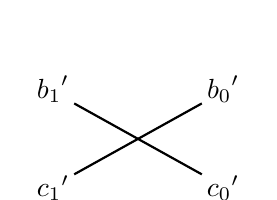
\begin{tikzpicture}[scale=0.9, baseline=(current bounding box.center)]
    \node at (0, 1.2) {${b_1}'$};
    \node at (2.4, 1.2) {${b_0}'$};
    \node at (0, -0.2) {${c_1}'$};
    \node at (2.4, -0.2) {${c_0}'$};
    \draw[thick] (0.3, 1.0) -- (2.1, 0.0);
    \draw[thick] (0.3, 0.0) -- (2.1, 1.0);
  \end{tikzpicture}
  \end{center}
  並交叉相乘，得 ${b_1}' {c_0}'$ 和 ${b_0}' {c_1}'$。
  \item[(三)] 驗證是否 ${b_1}' {c_0}' + {b_0}' {c_1}' = a_1$。如果是的話，則原二次式可寫為 $({b_1}' x + {b_0}')({c_1}' x + {c_0}')$，而其根也就求出來了。
  \item[(四)] 如果不是的話，以別的因數的積再試。
\end{enumerate}

以上方法對於根為整數時，才較為簡便，我們把上面的【例7】，【例8】用此法再做一遍：

\paragraph{【例7】} $x^2 + 3x - 18 = 0$。
\[
-18 = 6 \cdot (-3).
\]
\begin{center}
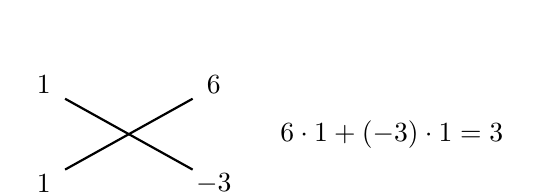
\begin{tikzpicture}[scale=0.9, baseline=(current bounding box.center)]
  \node at (0, 1.2) {$1$};
  \node at (2.4, 1.2) {$6$};
  \node at (0, -0.2) {$1$};
  \node at (2.4, -0.2) {$-3$};
  \draw[thick] (0.3, 1.0) -- (2.1, 0.0);
  \draw[thick] (0.3, 0.0) -- (2.1, 1.0);
  \node[anchor=west] at (3.2, 0.5) {$6 \cdot 1 + (-3) \cdot 1 = 3$};
\end{tikzpicture}
\end{center}
\[
(x+6)(x-3) = 0. \qquad \therefore\ x = -6,\ 3.
\]

\paragraph{【例8】} $6x^2 + x - 15 = 0$。
\begin{align*}
6 &= 3 \cdot 2, \\
-15 &= 5 \cdot (-3).
\end{align*}
\begin{center}
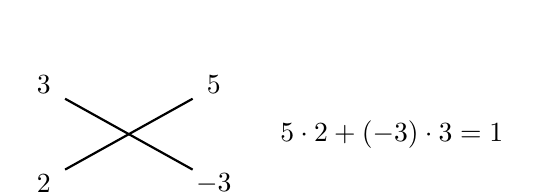
\begin{tikzpicture}[scale=0.9, baseline=(current bounding box.center)]
  \node at (0, 1.2) {$3$};
  \node at (2.4, 1.2) {$5$};
  \node at (0, -0.2) {$2$};
  \node at (2.4, -0.2) {$-3$};
  \draw[thick] (0.3, 1.0) -- (2.1, 0.0);
  \draw[thick] (0.3, 0.0) -- (2.1, 1.0);
  \node[anchor=west] at (3.2, 0.5) {$5 \cdot 2 + (-3) \cdot 3 = 1$};
\end{tikzpicture}
\end{center}
\[
(3x+5)(2x-3) = 0. \qquad \therefore\ x = -\frac{5}{3},\ \frac{3}{2}.
\]

\subsubsection*{習題 1-1}\label{sec:b2_ex1-1}

\begin{enumerate}
  \item 解下列各方程式：
  \begin{enumerate}[(i)]
    \item $x^2-3x+1=0$。
    \item $x^2+5x-4=0$。
    \item $x^2+20x+64=0$。
    \item $(x^2-6x+2)(x-1)(x+2)=0$。
    \item $(x^2+3x+1)(x^2-3x+1)=0$。
    \item $(x+5)^2=4x+20$。
    \item $x^4-25x^2+144=0$。
    \item $6x^4-5x^2+1=0$。
    \item $(2x^2-x)^2 - 4(2x^2-x) + 3 = 0$。
    \item $(2x^2-5x)^2+4x=10x+3$。
    \item $x-8\sqrt{x}+15=0$。
    \item $\sqrt{x}-29=-\dfrac{30}{\sqrt{x}}$。
  \end{enumerate}

  \item 用交叉因子分解法，解下列各方程式：
  \begin{enumerate}[(i)]
    \item $6x^2+x-2=0$。
    \item $20x^2-13x+2=0$。
    \item $21x^2+13x+2=0$。
    \item $20x^2-3x-9=0$。
  \end{enumerate}

  \item 把石頭用 $16.8$（公尺/秒）的初速度拋上去，那麼高度 $S$（公尺）是時間 $t$（秒）的二次函數。 $S=-490t^2+16.8t$\phantomsection\label{note:b2-ch1-gravity}，問什麼時候高度是 $14$ 公尺？

  \item 若將一立方體的各邊長增加 $2$ 公分，則其體積增加 $386$ 立方公分，求原來立方體的邊長。
\end{enumerate}

\subsection{配方與公式解}\label{sec:b2_1-2}

現在讓我們來討論一般解二次方程式的方法。設方程式為
\begin{equation}\label{eq:b2_quad_standard}\tag{1}
ax^2+bx+c=0,\ a \ne 0
\end{equation}
首先，我們可以將上式各項除以 $a$，而得下列首項係數為 $1$ 的式子：
\begin{equation}\label{eq:b2_quad_div_a}\tag{2}
x^2+\frac{b}{a}x+\frac{c}{a}=0
\end{equation}
又因
\begin{equation}\label{eq:b2_complete_square_id}\tag{3}
\left(x+\frac{b}{2a}\right)^2=x^2+\frac{b}{a}x+\left(\frac{b}{2a}\right)^2
\end{equation}
故(2)式可以重寫為
\[
\left(x+\frac{b}{2a}\right)^2 = \left(\frac{b}{2a}\right)^2 - \frac{c}{a} = \frac{b^2-4ac}{4a^2}.
\]
即得
\[
x+\frac{b}{2a} = \pm \sqrt{\frac{b^2-4ac}{4a^2}} = \frac{\pm \sqrt{b^2-4ac}}{2a}.
\]
亦即
\begin{equation}\label{eq:b2_quad_sol}\tag{4}
x = -\frac{b}{2a} \pm \frac{\sqrt{b^2-4ac}}{2a} = \frac{-b \pm \sqrt{b^2-4ac}}{2a}
\end{equation}

\paragraph{注意：}
\begin{enumerate}[(i)]
  \item 當 $b^2-4ac$ 是負數時，則 $\sqrt{b^2-4ac}$ 顯然不可能是一個實數，因為任何實數的平方總是 $\ge 0$。在這種情形下，我們叫 $\sqrt{b^2-4ac}$ 為一虛數。其意義將在以後再詳加闡述。
  \item 有些書在一開始就把 (1) 式寫成 $ax^2+2bx+c=0$，採用這樣的符號，則顯然有公式
  \[
  x = \frac{-b \pm \sqrt{b^2-ac}}{a}
  \]
  （以 $2b$ 代替 $b$，代入 (4) 式化簡即得）。
\end{enumerate}

我們把上述討論的結論，敘述為下列定理：

\begin{theorem}\label{thm:b2_1-1}
方程式
\[
ax^2+bx+c=0,\quad a \ne 0
\]
的根可以由下述公式求得：
\begin{equation}\label{eq:b2_quad_formula_thm}\tag{4}
x = \frac{-b \pm \sqrt{b^2-4ac}}{2a}
\end{equation}
\end{theorem}

\paragraph{注意：} 在求得上述公式的過程中，最要緊的是把 $x^2+\frac{b}{a}x$ 改寫成 $(x+\frac{b}{2a})^2 - \frac{b^2}{4a^2}$，即
\begin{equation}\label{eq:b2_completing_square_thm}\tag{5}
x^2+\frac{b}{a}x = \left(x+\frac{b}{2a}\right)^2 - \left(\frac{b}{2a}\right)^2
\end{equation}
這種步驟叫做配方，它在二次式的討論中是很重要的。

\begin{corollary}\label{cor:b2_1-1}
任意二次多項式 $ax^2+bx+c$，在形式上都可以作下列因子分解，即
\[
ax^2+bx+c = a\left(x - \frac{-b+\sqrt{b^2-4ac}}{2a}\right)\left(x - \frac{-b-\sqrt{b^2-4ac}}{2a}\right).
\]
\end{corollary}

\begin{corollary}\label{cor:b2_1-2}
任意二元二次齊次式 $ax^2+bxy+cy^2$，在形式上都可以作下列因式分解。即
\[
ax^2+bxy+cy^2 = a\left(x - \frac{-b+\sqrt{b^2-4ac}}{2a}y\right)\left(x - \frac{-b-\sqrt{b^2-4ac}}{2a}y\right).
\]
\hfill （證明留做習題）\phantomsection\label{note:b2-ch1-cor2}
\end{corollary}

\subsubsection*{習題 1-2}\label{sec:b2_ex1-2}

\begin{enumerate}
  \item 試證上面的推論 2.

  \item 用公式解下列方程式：
  \begin{enumerate}[(i)]
    \item $x^2+2x-1=0$。
    \item $x^2+x+1=0$。
    \item $(\sqrt{5}-2)x^2-2x+4=0$。
    \item $(x+2)(x+3)(x-4)=x^3$。
    \item $2x^2+3x=4$。
  \end{enumerate}

  \item 分解下列二次齊次式為一次因式：
  \begin{enumerate}[(i)]
    \item $3x^2-10xy+3y^2$。
    \item $x^2+xy+y^2$。
    \item $a^2-4ab+2b^2$。
    \item $2a^2-2ab-b^2$。
  \end{enumerate}
\end{enumerate}

\subsection{根與係數的關係、判別式與二次方程式的討論}\label{sec:b2_1-3}

\subsubsection*{3-1 本節符號用法}

在這一節裡，我們將依然用 $ax^2+bx+c=0$ 表示一個一般的二次方程式。我們將用 $\alpha, \beta$ 表示它的根，以 $\delta$ 表示 $b^2-4ac$。即
\[
\delta = b^2-4ac,
\]
這式叫做該方程式的判別式。

\subsubsection*{3-2 根與係數的關係}

設 $\alpha, \beta$ 為 $ax^2+bx+c=0$ 的根，則由餘式定理得
\begin{align*}
ax^2+bx+c &= a\cdot \left(x^2+\frac{b}{a}x+\frac{c}{a}\right) \\
&= a\cdot (x-\alpha)(x-\beta) \\
&= a\cdot [x^2-(\alpha+\beta)x+\alpha\beta].
\end{align*}
依多項式相等的定義，上面左右兩邊各項係數應該相等。故有下述根與係數關係：
\[
\alpha+\beta = -\frac{b}{a},
\]
\[
\alpha\beta = \frac{c}{a}.
\]

\begin{example}\label{ex:b2_1-3-1}
設 $\alpha, \beta$ 為二次方程式 $2x^2+3x+6=0$ 的兩根，則有
\begin{align*}
\alpha+\beta &= -\frac{3}{2}, \\
\alpha\beta &= 3.
\end{align*}
\end{example}

\begin{example}\label{ex:b2_1-3-2}
求以 $\dfrac{p-q}{p+q}$ 與 $\dfrac{-(p+q)}{p-q}$ 為兩根的二次方程式。
\end{example}
\paragraph{【解】}
設兩根為 $\alpha$ 與 $\beta$，則
\begin{align*}
\alpha+\beta &= \frac{p-q}{p+q} - \frac{p+q}{p-q} = \frac{(p-q)^2 - (p+q)^2}{p^2-q^2} \\
&= \frac{-4pq}{p^2-q^2}, \\
\alpha\beta &= \frac{p-q}{p+q} \cdot \left(-\frac{p+q}{p-q}\right) = -1.
\end{align*}
所以
\[
x^2 + \frac{4pq}{p^2-q^2}x - 1 = 0 \text{ 以 } \alpha, \beta \text{ 為根}.
\]
\[
\therefore \quad (p^2-q^2)x^2 + 4pqx - (p^2-q^2) = 0
\]
為我們所求的一個方程式。


\begin{example}\label{ex:b2_1-3-3}
設 $ax^2+bx+c=0$ 的兩根之比為 $m:n$，試證
\[
mnb^2 = (m+n)^2 ac.
\]
\end{example}
\paragraph{【解】}
設兩根為 $m\alpha, n\alpha$。由根與係數的關係得
\begin{align}
(m+n)\alpha &= -\frac{b}{a} \tag{1}\label{eq:b2_root_ratio_sum} \\
mn\alpha^2 &= \frac{c}{a} \tag{2}\label{eq:b2_root_ratio_prod}
\end{align}
由 \eqref{eq:b2_root_ratio_sum} 得 $\alpha = \dfrac{-b}{(m+n)a}$，代入 \eqref{eq:b2_root_ratio_prod} 式得
\[
mn\left[\frac{-b}{a(m+n)}\right]^2 = \frac{c}{a}
\]
通分得 $mnb^2 = (m+n)^2 ac$，故得證。


\subsubsection*{3-3 二次方程式的討論}

在上節公式 (4) $x = \dfrac{-b \pm \sqrt{b^2-4ac}}{2a}$ 可知兩根相等的充分必要條件是 $\delta = b^2-4ac = 0$。而當 $\delta > 0$ 時，$ax^2+bx+c=0$ 有相異的二實根，當 $\delta < 0$ 時，其根為 $\dfrac{-b \pm \sqrt{b^2-4ac}}{2a}$ 的形式，其中 $\sqrt{b^2-4ac}$ 為一虛數。習慣上，這種根叫做虛根。

綜合上述討論，可敘述為下列定理。

\begin{theorem}\label{thm:b2_1-2}
對於二次方程式 $ax^2+bx+c=0$，$a \ne 0$。根與係數間有下列關係：
\begin{enumerate}[(i)]
  \item 二根之和為 $-\frac{b}{a}$，二根之積為 $\frac{c}{a}$（即 $\alpha+\beta = -\frac{b}{a}$，$\alpha\beta = \frac{c}{a}$）。
  \item
  \[
  \begin{cases}
  \delta = 0 \iff \text{有二相等實根（亦稱為二重根）}. \\
  \delta > 0 \iff \text{有二相異實根}. \\
  \delta < 0 \iff \text{有二相異虛根}.
  \end{cases}
  \]
\end{enumerate}
\end{theorem}

\begin{example}\label{ex:b2_1-3-4}
設 $x^2+8x+q=0$ 的二根之差的平方為 $4$，求 $q$ 的值。
\end{example}
\paragraph{【解】}
令 $\alpha, \beta$ 為上述方程式的二根，則由假設得
\[
(\alpha-\beta)^2 = 4.
\]
但是由等式 $(\alpha-\beta)^2 = \alpha^2-2\alpha\beta+\beta^2 = (\alpha^2+2\alpha\beta+\beta^2)-4\alpha\beta = (\alpha+\beta)^2-4\alpha\beta$，故由根與係數的關係即得
\[
4 = 8^2-4q = 64-4q,\qquad q=15.
\]


\begin{example}\label{ex:b2_1-3-5}
設 $x^2+px+q=0$ 的二根為 $\alpha, \beta$。求以 $\alpha^2+\beta$ 和 $\beta^2+\alpha$ 為根的二次方程式。
\end{example}
\paragraph{【解】}
設所求的方程式為 $x^2+bx+c=0$，則根與係數的關係為
\[
\begin{cases}
(\alpha^2+\beta)+(\beta^2+\alpha) = -b \\
(\alpha^2+\beta)\cdot(\beta^2+\alpha) = c
\end{cases}, \qquad
\begin{cases}
\alpha+\beta = -p \\
\alpha\beta = q
\end{cases}.
\]
我們得把 $b, c$ 用原方程式的係數 $p, q$ 表出。換言之，我們得設法把 $\alpha^2+\beta^2+\alpha+\beta$ 和 $\alpha^2\beta^2+\alpha\beta+\alpha^3+\beta^3$ 用 $\alpha+\beta$ 和 $\alpha\beta$ 表出，同學們不難由展開得下述等式：
\begin{align*}
(\alpha+\beta)^2 &= \alpha^2+2\alpha\beta+\beta^2; \\
\text{即}\qquad \alpha^2+\beta^2 &= (\alpha+\beta)^2-2\alpha\beta. \\
(\alpha+\beta)^3 &= \alpha^3+3\alpha^2\beta+3\alpha\beta^2+\beta^3, \\
\text{即}\qquad \alpha^3+\beta^3 &= (\alpha+\beta)^3-3\alpha\beta\cdot(\alpha+\beta).
\end{align*}
故有
\begin{align*}
-b &= (\alpha^2+\beta^2)+(\alpha+\beta) = (\alpha+\beta)^2-2\alpha\beta+(\alpha+\beta) \\
&= p^2-p-2q. \\
c &= \alpha^2\beta^2+\alpha\beta+(\alpha^3+\beta^3) = (\alpha\beta)^2+\alpha\beta+(\alpha+\beta)^3 - 3\alpha\beta(\alpha+\beta) \\
&= q^2+q+3qp-p^3.
\end{align*}
亦即所求方程式為
\[
x^2-(p^2-p-2q)x + (q^2+q+3qp-p^3) = 0.
\]


\subsubsection*{習題 1-3}\label{sec:b2_ex1-3}

\begin{enumerate}
  \item 找一個整係數二次方程式，使它的根是：
  \begin{enumerate}[(i)]
    \item $-3, 8$。
    \item $\dfrac{1}{2}, -\dfrac{5}{3}$。
    \item $-1+\sqrt{2}, -1-\sqrt{2}$。
    \item $-2+\sqrt{3}, -2-\sqrt{3}$。
  \end{enumerate}

  \item 甲，乙兩人解同一個二次方程式，甲將第二項 $x$ 的係數看錯，解得二根為 $-3, -4$；乙將第三項常數看錯，解得二根為 $2, 5$；你的答案是多少？

  \item 如果 $ax^2+bx+c=0$ 的兩根是 $\alpha, \beta$，找一個二次方程式，使它的根是：
  \begin{enumerate}[(i)]
    \item $2\alpha, 2\beta$。
    \item $\alpha+1, \beta+1$。
    \item $\alpha^2, \beta^2$。
    \item $\dfrac{1}{\alpha}, \dfrac{1}{\beta}$。
  \end{enumerate}

  \item 如果 $ax^2+bx+c=0$ 的根是 $\alpha, \beta$，請用 $a, b, c$ 表示
  \begin{enumerate}[(i)]
    \item $\dfrac{1}{\alpha} + \dfrac{1}{\beta}$。
    \item $(\alpha-1)(\beta-1)$。
    \item $\dfrac{\beta}{\alpha} + \dfrac{\alpha}{\beta}$。
    \item $\alpha^3 + \beta^3$。
  \end{enumerate}

  \item 試證 $(a+b)x^2 - (a+b+c)x + \dfrac{c}{2} = 0$ 有實根。
\end{enumerate}

\subsection{應用}\label{sec:b2_1-4}

\subsubsection*{4-1 二次函數的極大、極小}

在第一冊第五章中我們說過：任何一個多項式 $f(x)$，都有一個對應的多項式函數 $y=f(x)$；因此對於一個二次多項式 $ax^2+bx+c$，我們有一個對應的二次函數
\begin{equation}\label{eq:b2_quad_func}\tag{1}
y = ax^2+bx+c
\end{equation}
由 \S 2 配方的計算，我們可以把(1)式重寫為
\begin{align}
y &= a\left[\left(x+\frac{b}{2a}\right)^2 + \frac{4ac-b^2}{4a^2}\right] \nonumber \\
&= a\left[\left(x+\frac{b}{2a}\right)^2 + \frac{(-\delta)}{4a^2}\right] \tag{2}\label{eq:b2_quad_vertex}
\end{align}
顯然，當 $x$ 為任何實數時，均有
\begin{equation}\label{eq:b2_square_nonneg}\tag{3}
\left(x+\frac{b}{2a}\right)^2 \ge 0, \text{（``$=$''僅在 $x=-\frac{b}{2a}$ 時成立）}
\end{equation}
故有
\[
\left(x+\frac{b}{2a}\right)^2 + \frac{-\delta}{4a^2} \ge \frac{-\delta}{4a^2}, \text{（``$=$''僅於 $x=-\frac{b}{2a}$ 時成立）}
\]
所以當 $a > 0$ 時，我們有
\[
y = a\cdot \left[\left(x+\frac{b}{2a}\right)^2 + \frac{-\delta}{4a^2}\right] \ge \frac{-\delta}{4a^2}\cdot a = \frac{-\delta}{4a} = f\left(-\frac{b}{2a}\right).
\]
亦即當 $a>0$ 時，二次函數 $y=ax^2+bx+c$ 在 $x=-\frac{b}{2a}$ 時的函數值
\[
f\left(-\frac{b}{2a}\right) = \frac{-\delta}{4a} = \frac{4ac-b^2}{4a}
\]
是該函數的極小值。反之，當 $a<0$ 時，我們有
\[
y = a\cdot \left[\left(x+\frac{b}{2a}\right)^2 + \frac{-\delta}{4a^2}\right] \le \frac{-\delta}{4a^2}\cdot a = \frac{-\delta}{4a} = f\left(-\frac{b}{2a}\right).
\]
亦即當 $a<0$ 時，二次函數 $y=ax^2+bx+c$ 在 $x=-\frac{b}{2a}$ 時的函數值 $f\left(-\frac{b}{2a}\right) = \frac{-\delta}{4a}$ 是它的極大值。

\begin{theorem}\label{thm:b2_1-3}
二次函數 $y=ax^2+bx+c$ 在 $x=-\frac{b}{2a}$ 時的函數值
\[
f\left(-\frac{b}{2a}\right) = \frac{-\delta}{4a} = \frac{4ac-b^2}{4a}
\]
不是極大就是極小：當 $a<0$ 時為極大；$a>0$ 時為極小。
\end{theorem}

\begin{corollary}\label{cor:b2_1-3}
對於一個二次函數 $y=ax^2+bx+c$，
\begin{enumerate}[(i)]
  \item 其函數值永不為負（亦即 $f(x)$ 永遠 $\ge 0$）的充分必要條件是「$a>0$ 和 $\delta \le 0$」。
  \item 其函數值永不為正（亦即 $f(x)$ 永遠 $\le 0$）的充分必要條件是「$a<0$ 和 $\delta \le 0$」。
\end{enumerate}
\end{corollary}

\begin{example}\label{ex:b2_1-4-1}
今有一 $400$ 公尺長的鐵絲網一捲，用來圍一塊長方形的地，問最多可以圍多少平方公尺？
\end{example}
\paragraph{【解】}
令 $x$ 為此長方形的寬，則 $\frac{1}{2}(400-2x) = 200-x$ 為其長，故長方形的面積為
\[
y = x\cdot (200-x) = -x^2+200x.
\]

\begin{figure}[htbp]
\centering
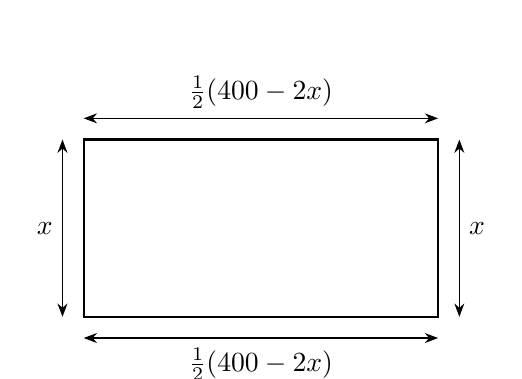
\begin{tikzpicture}[scale=0.9, >=Stealth]
  \draw[thick] (0, 0) rectangle (5, 2.5);
  % 寬度標註
  \draw[<->] (-0.3, 0) -- (-0.3, 2.5) node[midway, left] {$x$};
  \draw[<->] (5.3, 0) -- (5.3, 2.5) node[midway, right] {$x$};
  % 長度標註
  \draw[<->] (0, 2.8) -- (5, 2.8) node[midway, above] {$\frac{1}{2}(400-2x)$};
  \draw[<->] (0, -0.3) -- (5, -0.3) node[midway, below] {$\frac{1}{2}(400-2x)$};
\end{tikzpicture}
\caption{鐵絲網圍成長方形示意圖}
\label{fig:fenced_field}
\end{figure}

由定理3，當 $x = \frac{-b}{2a} = 100$ 時，上述函數得其極大值 $10000 = f(100)$，故當所圍者是一個 $100 \times 100$ 的正方形時，面積最大，共計 $10000$ 平方公尺。


\begin{example}\label{ex:b2_1-4-2}
今有一高射砲彈，它在出砲口時的「垂直分速」是 $400$ 公尺/秒。「水平分速」是 $100$ 公尺/秒。若將空氣阻力略去不計時，試求它的「彈道」（註\footnote{砲彈飛行所經過的軌跡，軍事術語叫做彈道，在數學中，這一類由拋擲物體所成的軌跡叫做拋物線，其種種性質將在以後再詳加討論。}）的「最高點」的高度？它落地時和原砲位的水平距離？
\end{example}
\paragraph{【解】}
對於上述物理問題，地心引力是影響該砲彈飛行的最主要因素。（其次要者如空氣阻力，氣流速度等均已略去不計。）它使砲彈在垂直方向產生 $-9.8$ 公尺/秒$^2$ 的加速度，故砲彈在垂直方向的投影是一個加速度為 $-9.8$ 公尺/秒$^2$ 的等加速運動，由等加速運動的距離公式有
\[
y = t\text{ 秒的高度} = \left(400\cdot t - \frac{1}{2}(9.8)\cdot t^2\right) \text{ 公尺}.
\]
由定理 3 得知，當 $t = \frac{-b}{2a}$ 秒時砲彈達最高點，其高度為
\[
f\left(-\frac{b}{2a}\right) = \frac{4ac-b^2}{4a} = \frac{(400)^2}{2\cdot(9.8)} = 8163\text{ 公尺}.
\]
即最高點的高度約為 $8163$ 公尺。

\begin{figure}[htbp]
\centering
\begin{tikzpicture}[scale=1.1, >=Stealth]
  % 坐標軸
  \draw[->, thick] (0, 0) -- (0, 5.5);
  \node[left] at (-0.05, 3.2) {\shortstack{高\\度}};
  \draw[->, thick] (0, 0) -- (6.5, 0);
  \node[below] at (3.2, -0.1) {水平距離};

  % 拋物線彈道
  \draw[very thick] (0, 0) parabola bend (2.8, 4.8) (5.6, 0);

  % 重力向下箭頭
  \draw[->, very thick] (2.8, 3.8) -- (2.8, 2.6);
  \node[below] at (2.8, 2.5) {\shortstack{重\\力}};
\end{tikzpicture}
\caption{拋射物體彈道示意圖}
\label{fig:trajectory}
\end{figure}

因水平方向的運動是不受地心引力的影響的，所以其水平投影是一個等速運動，即
\[
t\text{ 秒的水平距離} = (100\cdot t)\text{ 公尺}
\]
由 $y = 400t - \frac{1}{2}(9.8)\cdot t^2 = 0$ 可以求得其落地的時間為
\[
t = \frac{400}{4.9} = 81.63\text{ 秒}.
\]
故落地時的水平距離為
\[
100\cdot (81.63) = 8163 \text{ 公尺}.
\]

\begin{example}\label{ex:b2_1-4-3}
設 $a_1, a_2, a_3, b_1, b_2, b_3$ 為任意實數，則顯然下述函數值永不為負。
\end{example}
\paragraph{【解】}
\begin{align*}
y &= (a_1 x+b_1)^2 + (a_2 x+b_2)^2 + (a_3 x+b_3)^2 \\
&= (a_1^2+a_2^2+a_3^2)x^2 + 2\cdot (a_1 b_1 + a_2 b_2 + a_3 b_3)x + (b_1^2+b_2^2+b_3^2) \ge 0.
\end{align*}
故由推論，即得
\[
\delta = 4\cdot (a_1 b_1 + a_2 b_2 + a_3 b_3)^2 - 4\cdot (a_1^2+a_2^2+a_3^2)(b_1^2+b_2^2+b_3^2) \le 0
\]
亦即
\[
(a_1 b_1 + a_2 b_2 + a_3 b_3)^2 \le (a_1^2+a_2^2+a_3^2)(b_1^2+b_2^2+b_3^2)
\]
上述不等式叫做舒瓦茲（Schwarz）不等式，它和幾何中的「三角形兩邊的和大于第三邊」具有密切關連。以後我們還會對此詳加剖析的。


\subsubsection*{習題 1-4}\label{sec:b2_ex1-4}

\begin{enumerate}
  \item 求下列各方程式的極大或極小：
  \begin{enumerate}[(i)]
    \item $y = 2x^2-x+4$。
    \item $y = -5x^2-4x+2$。
    \item $y = x(x+1)$。
    \item $y = -x^2-3x+2$。
    \item $y = -7x^2+6x-1$。
  \end{enumerate}

  \item 求內接於圓而面積最大的矩形，和周界最大的矩形。

  \item 設線段 $\overline{AB}$ 的長是 $a$，在 $\overline{AB}$ 上任取一點 $P$，以線段 $\overline{AB}$ 和 $\overline{PB}$ 為一邊各作一正方形\phantomsection\label{note:b2-ch1-ex1-4-q3}. 如果要使這兩個正方形面積的和為最小，試求 $P$ 點的位置應該在那裏？

  \item 如下圖，$\overline{AB}$ 是一條長 $24$ 公分的鐵絲，$P$ 是 $\overline{AB}$ 上一點，將 $\overline{PB}$ 分為四等分，使它圍成一正方形 $PSTU$；將 $AP$ 分為三等分，使其實成一正三角形 $PQR$\phantomsection\label{note:b2-ch1-ex1-4-q4}. $R, U, P$ 三點決定一三角形，問 $P$ 在何處時 $\triangle UPR$ 面積最大。

  \begin{figure}[htbp]
  \centering
  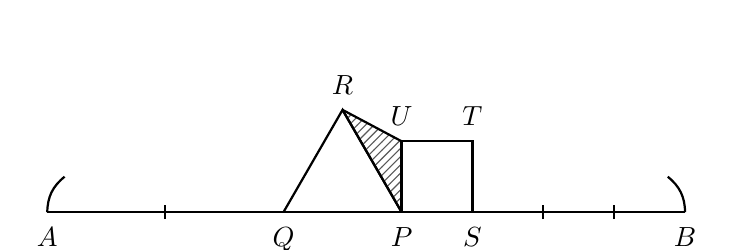
\begin{tikzpicture}[scale=1.0, >=Stealth]
    % 基準線 AB：AP 三等分（每段 1.5），PB 四等分（每段 0.9）
    \coordinate (A) at (-4.5, 0);
    \coordinate (M1) at (-3.0, 0);
    \coordinate (Q) at (-1.5, 0);
    \coordinate (P) at (0, 0);
    \coordinate (S) at (0.9, 0);
    \coordinate (N1) at (1.8, 0);
    \coordinate (N2) at (2.7, 0);
    \coordinate (B) at (3.6, 0);

    \draw[thick] (A) -- (B);

    % 等分點刻度（AQ 間一處，SB 間兩處）
    \foreach \pt in {M1, N1, N2} {
      \draw[thick] (\pt) ++(0, -0.09) -- ++(0, 0.18);
    }

    % 正三角形 PQR (邊長 QP = 1.5，高 = 1.299 > 0.9)
    \coordinate (R) at (-0.75, 1.299);
    \draw[thick] (Q) -- (R) -- (P);

    % 正方形 PSTU (邊長 PS = 0.9)
    \coordinate (T) at (0.9, 0.9);
    \coordinate (U) at (0, 0.9);
    \draw[thick] (P) -- (S) -- (T) -- (U) -- cycle;

    % 陰影三角形 UPR
    \fill[pattern=north east lines, pattern color=black!65] (U) -- (P) -- (R) -- cycle;
    \draw[thick] (U) -- (R);
    \draw[thick] (U) -- (P);
    \draw[thick] (P) -- (R);

    % 端點彎折弧線（貼齊 A、B 兩端點向上向內彎起）
    \draw[thick] (A) to[bend left=25] ++(0.22, 0.45);
    \draw[thick] (B) to[bend right=25] ++(-0.22, 0.45);

    % 標籤
    \node[below=2pt] at (A) {$A$};
    \node[below=2pt] at (Q) {$Q$};
    \node[below=2pt] at (P) {$P$};
    \node[below=2pt] at (S) {$S$};
    \node[below=2pt] at (B) {$B$};

    \node[above=2pt] at (R) {$R$};
    \node[above=2pt] at (U) {$U$};
    \node[above=2pt] at (T) {$T$};
  \end{tikzpicture}
  \caption{正三角形與正方形幾何配置圖}
  \label{fig:triangle_square}
  \end{figure}

  \item 設 $y$ 為 $x$ 之二次多項式，而當 $x=0, 1, 2$ 時，$y$ 分別為 $8, 5, 6$，試求 $y$。
\end{enumerate}

\subsubsection*{4-2 二次聯立方程式}

就如同解二元、三元一次聯立方程式，我們可以用同樣的原則，和上幾節所學到的二次方程式解法，去解二次聯立方程式。現在我們舉例如下：

\begin{example}\label{ex:b2_1-4-4}
解二次聯立方程式
\[
\begin{cases}
x^2+y^2=34 \dots\dots\dots\dots\dots\dots\dots\dots\dots\dots (1) \\
y=x+2 \dots\dots\dots\dots\dots\dots\dots\dots\dots\dots (2)
\end{cases}
\]
\end{example}
\paragraph{【解】}
將 (2) 代入 (1) 得
\begin{align*}
x^2+(x+2)^2 &= 34 \\
2x^2+4x+4 &= 34 \\
\text{即}\qquad x^2+2x-15 &= 0 \\
(x-3)(x+5) &= 0 \\
\therefore\quad x=3,\ x=-5.
\end{align*}
將此二解分別代入 (2)
\begin{align*}
y &= x+2 = 3+2=5 \\
y &= x+2 = -5+2=-3
\end{align*}
故此聯立方程式的解為
\[
\begin{cases} x=3 \\ y=5, \end{cases}\qquad
\begin{cases} x=-5 \\ y=-3. \end{cases}
\]


\begin{example}\label{ex:b2_1-4-5}
解二次聯立方程式
\[
\begin{cases}
6x^2-xy-2y^2=0 \dots\dots\dots\dots\dots\dots\dots\dots\dots\dots (1) \\
4x^2+xy-4y^2=-14 \dots\dots\dots\dots\dots\dots\dots\dots\dots\dots (2)
\end{cases}
\]
\end{example}
\paragraph{【解】}
將 (1) 分解因式，得
\[
(3x-2y)(2x+y)=0
\]
\begin{align}
y &= \frac{3}{2}x \tag{3}\label{eq:b2_sim_y1} \\
y &= -2x \tag{4}\label{eq:b2_sim_y2}
\end{align}
將 \eqref{eq:b2_sim_y1} 代入 (2)，得
\begin{align*}
4x^2+x\cdot \frac{3}{2}x - 4\cdot \left(\frac{3}{2}x\right)^2 &= -14 \\
4x^2+\frac{3}{2}x^2-9x^2 &= -14 \\
8x^2+3x^2-18x^2 &= -28 \\
7x^2 &= 28 \\
\text{即}\qquad x^2 &= 4 \\
\therefore\quad x &= \pm 2
\end{align*}
$x=2$ 代入 \eqref{eq:b2_sim_y1} 得
\[
y = \frac{3}{2}\cdot 2 = 3
\]
$x=-2$ 代入 \eqref{eq:b2_sim_y1} 得
\[
y = \frac{3}{2}(-2) = -3
\]
將 \eqref{eq:b2_sim_y2} 代入 (2) 得
\begin{align*}
4x^2+x\cdot(-2x)-4(2x)^2 &= -14 \\
4x^2-2x^2-16x^2 &= -14 \\
14x^2 &= 14 \\
x^2 &= 1 \\
\therefore\quad x &= \pm 1.
\end{align*}
$x=1$ 代入 \eqref{eq:b2_sim_y2}，得
\[
y = -2.
\]
$x=-1$ 代入 \eqref{eq:b2_sim_y2}，得
\[
y = 2.
\]
故其解為
\[
\begin{cases} x=2 \\ y=3, \end{cases}\qquad
\begin{cases} x=-2 \\ y=-3, \end{cases}\qquad
\begin{cases} x=1 \\ y=-2, \end{cases}\qquad
\begin{cases} x=-1 \\ y=2. \end{cases}
\]


\begin{example}\label{ex:b2_1-4-6}
解三元聯立方程式
\[
\begin{cases}
y^2-xy-yz=3 \dots\dots\dots\dots\dots\dots\dots\dots\dots\dots (1) \\
x+4y+z=14 \dots\dots\dots\dots\dots\dots\dots\dots\dots\dots (2) \\
x-y+2z=0 \dots\dots\dots\dots\dots\dots\dots\dots\dots\dots (3)
\end{cases}
\]
\end{example}
\paragraph{【解】}
(3)-(2) 得
\[
-5y+z=-14
\]
\begin{equation}\label{eq:b2_sim3_z}\tag{4}
z=5y-14
\end{equation}
$2 \times (2) - (3)$ 得
\[
x+9y=28
\]
\begin{equation}\label{eq:b2_sim3_x}\tag{5}
x=28-9y
\end{equation}
將 \eqref{eq:b2_sim3_z}, \eqref{eq:b2_sim3_x} 代入 (1) 得
\begin{align*}
y^2-(28-9y)y-y(5y-14) &= 3 \\
y^2-28y+9y^2-5y^2+14y &= 3 \\
5y^2-14y-3 &= 0 \\
(5y+1)(y-3) &= 0 \\
\therefore\quad y=-\frac{1}{5},\quad y=3
\end{align*}
將 $y=-\frac{1}{5}$ 代入 \eqref{eq:b2_sim3_z} 得\phantomsection\label{note:b2-ch1-ex6-sign}
\[
z=5\cdot\left(\frac{1}{5}\right)-14=-15
\]
$y=3$ 代入 \eqref{eq:b2_sim3_z} 得
\[
z=5(+3)-14=1
\]
將 $y=-\frac{1}{5}$ 代入 \eqref{eq:b2_sim3_x} 得
\[
x=28-9\cdot\left(-\frac{1}{5}\right) = 28+\frac{9}{5} = 29\frac{4}{5}
\]
$y=3$ 代入 \eqref{eq:b2_sim3_x} 得
\[
x = 28-9\cdot 3 = 1
\]
故其解為
\[
\begin{cases}
x=1 \\
y=3 \\
z=1,
\end{cases}\qquad
\begin{cases}
x=29\dfrac{4}{5} \\
y=-\dfrac{1}{5} \\
z=-15.
\end{cases}
\]


\begin{example}\label{ex:b2_1-4-7}
在一塊正方形的土地上造一座長方形的游泳池。泳池的面積為土地面積的三分之一，泳池的長比寬大 $26$ 公尺，但比土地的邊長小 $10$ 公尺；求土地的面積以及泳池的長與寬。
\end{example}
\paragraph{【解】}
設泳池的長為 $x$，寬為 $y$，土地的邊長為 $z$。由題意得
\[
\begin{cases}
3xy = z^2 \dots\dots\dots\dots\dots\dots\dots\dots\dots\dots (1) \\
x-y = 26 \dots\dots\dots\dots\dots\dots\dots\dots\dots\dots (2) \\
z-x = 10 \dots\dots\dots\dots\dots\dots\dots\dots\dots\dots (3)
\end{cases}
\]
由 (2) 及 (3) 式得
\begin{equation}\label{eq:b2_pool_xy}\tag{4}
x = z-10,\quad y = z-36,
\end{equation}
代入 (1) 式化簡後得
\[
z^2-60z = 0
\]
解出 $z = 0, 60$。 $z=0$ 不合題意，\\
所以 $z=60$。\\
代入 \eqref{eq:b2_pool_xy} 式得
\[
x=50,\quad y=24.
\]
答：土地面積為 $3600$ 平方公尺。泳池的長為 $50$ 公尺，寬為 $24$ 公尺。


\subsubsection*{習題 1-5}\label{sec:b2_ex1-5}

\begin{enumerate}
  \item 解下列二次聯立方程式：
  \begin{multicols}{2}
  \begin{enumerate}[(i)]
    \item $\begin{cases}
    7x^2-6xy=8 \\
    2x-3y=5
    \end{cases}$

    \item $\begin{cases}
    xy=1 \\
    3x-5y=2
    \end{cases}$

    \item $\begin{cases}
    x^2+xy-6=0 \\
    x^2-5x+6=0
    \end{cases}$

    \item $\begin{cases}
    x^2+y-8=0 \\
    -y^2+15x-46=0
    \end{cases}$

    \item $\begin{cases}
    x^2+xy-2y^2=0 \\
    11x^2+3xy-11y^2=27
    \end{cases}$

    \item $\begin{cases}
    3x-2y+z=7 \\
    2x+y-z=-1 \\
    x^2+y^2+z^2=6
    \end{cases}$

    \item $\begin{cases}
    x+y+z=4 \\
    2x-y+z=8 \\
    xy+z=1
    \end{cases}$

    \item $\begin{cases}
    x^2+xy+x=10 \\
    y^2+xy+y=20
    \end{cases}$

    \item $\begin{cases}
    x^2+xy+y^2=13 \\
    x^2-xy+y^2=7
    \end{cases}$

    \item $\begin{cases}
    x^2+xy=36 \\
    y^2+xy=45
    \end{cases}$

    \item $\begin{cases}
    (x+1)(2y+1) = 5x+9y=1 \\
    (x+2)(3y+1) = 9x+13y+2
    \end{cases}$\phantomsection\label{note:b2-ch1-ex1-5-q1-11}
  \end{enumerate}
  \end{multicols}

  \item 有一矩形面積為 $162$ 平方公分，如果其寬加多 $3$ 公分，長減少 $3$ 公分，那麼面積增加 $18$ 平方公分，求這矩形的長與寬。

  \item 兩數的積等於和，又等於兩數的平方差，問此兩數為何？
\end{enumerate}
 % 第一章 二次方程式
% =========================================================================
% 《高中數學實驗教材》第二冊（高一下） 
% 第二章 次序與極限觀念
% =========================================================================

\section{次序與極限觀念}\label{sec:b2_ch2}

「數系」的概念由於對於各種「量」的問題作有系統的討論而產生。例如：吃了一根香蕉再吃一根香蕉，共吃了兩根香蕉，是一個日常生活的經驗，將它抽象化之後，我們便得到 $1+1=2$。所以由「量與量之間的相加」抽象出來「數與數之間的加法運算」。在第一冊第三章中，我們更談到如何以「加法運算」為基礎，逐步衍生出「減」、「乘」、「除」等運算。日常生活的量與量之間，除了可以相加之外，還常有很自然的「大小」關係。將這些關係抽象化，即得「數與數之間的次序關係」（亦即 $>$ 或 $<$ 關係）。運算與次序關係是數系的兩種基本結構。

以數系在運算上所具有的基本性質為出發點，在上一冊以及這一冊的第一章中，我們討論過整數的因子分解、多項式的運算與因子分解以及一次、二次方程式的理論及應用。本章將以數系在「次序關係」上的基本性質為出發點，逐步討論不等式與極限觀念。同學們將會看出極限觀念也就是次序關係在觀念上的一種推廣。

\subsection{次序與不等式的基本性質}\label{sec:b2_2-1}

\subsubsection*{1-1 次序與正負}

在日常生活中，我們說 $A$ 量大於 $B$ 量的意義是：「從 $A$ 量減去 $B$ 量後還有剩餘。」所以在數系中我們定義「$a$ 大於 $b$」的意義為「$a-b$ 是一正數」。也就是
\begin{definition*}
$a>b \iff a-b \text{ 是一正數}.$
\[
a<b \iff a-b \text{ 是一負數}.
\]
所以 $a>b$ 與 $b<a$ 是同一回事。
\end{definition*}

\paragraph{注意：} 由上述定義，我們有下面的特例
\begin{align*}
a>0 &\iff a \text{ 為一正數}, \\
a<0 &\iff a \text{ 為一負數}.
\end{align*}
這種正負數的表示法，前面已經用過。

在整數系、有理數系及實數系中，顯然都具有下列性質。即
\begin{enumerate}[(i)]
    \item 正數加正數仍為正數。
    \item 正數乘正數仍為正數。
    \item 正數乘負數則為負數。\quad （符號定則）
    \item 負數乘負數則為正數。
    \item 任何一數或為正，或為零，或為負；且上述三種可能性互斥。
\end{enumerate}

\subsubsection*{1-2 不等式的基本性質}

基於上述五點關於正、負數的性質，我們說明不等式的基本性質如下：
\begin{enumerate}[(1)]
    \item $a>b \text{ 和 } b>c \implies a>c$。
\paragraph{【證明】} $a>b \text{ 和 } b>c \implies a-b>0 \text{ 和 } b-c>0$
    \[
    \overset{\text{(i)}}{\implies} a-c = (a-b)+(b-c) > 0 \implies a>c.
    \]

    \item 對任何兩數 $a, b$，由 (v) 可知下列關係有一種且僅有一種成立：
    \[
    a>b,\quad a=b,\quad \text{或 } a<b.
    \]

    \item $a>b \iff a+c > b+c$。\quad （註\footnote{性質 (3) 表示加法的對消法則對不等式也成立，因此移項法則也成立。}）
\paragraph{【證明】} 
    \begin{align*}
    a>b &\iff a-b=(a+c)-(b+c)>0 \\
    &\iff a+c>b+c.
    \end{align*}

    \item $a>b \text{ 和 } c>d \implies a+c>b+d$。
\paragraph{【證明】} 
    \begin{align*}
    a>b \text{ 和 } c>d &\implies a+c>b+c \text{ 和 } b+c>b+d \\
    &\overset{\text{(1)}}{\implies} a+c>b+d.
    \end{align*}

    \item $a>b \text{ 和 } c>0 \implies ac>bc$。
\paragraph{【證明】} 
    \begin{align*}
    a>b \text{ 和 } c>0 &\implies a-b>0, \text{ 和 } c>0. \\
    &\overset{\text{(ii)}}{\implies} ac-bc = (a-b)\cdot c > 0. \\
    &\implies ac>bc.
    \end{align*}

    \item $a>b \text{ 和 } c<0 \implies ac<bc$。

    \item $a>b>0,\ c>d>0 \implies ac>bd$。
\end{enumerate}

\begin{example}\label{ex:b2_2-1-1}
所有的正整數可以按大小次序排為 $1<2<3<\dots < k < k+1 < \dots$。
\end{example}

\begin{example}\label{ex:b2_2-1-2}
因為 $9>-13$，用上面的性質 (5) 得到 $9\times (-8) > (-13)\times(-8)$ 也就是 $-72>104$，錯誤在那裏？
\end{example}

\begin{example}\label{ex:b2_2-1-3}
對任意的正有理數 $a, b$，我們可以找到一個正整數 $n$，滿足 $na>b$。
\end{example}
\paragraph{【證明】} 先假定 $a, b$ 都是正整數，我們利用正整數的除法，得到
\[
b=ka+r \qquad 0\le r < a
\]
如果讓 $n=k+1$，我們有
\[
(k+1)a-b = (k+1)a-ka-r = a-r > 0
\]
如果現在 $a=\frac{p}{q},\ b=\frac{r}{s}$，且 $q>0,\ s>0,\ p>0,\ r>0$。

因為 $a=\frac{ps}{sq}$ 和 $b=\frac{pr}{sq}$ 且 $sq>0, ps>0, pr>0$\phantomsection\label{note:b2-ch2-p28-ex3-pr}，如果找到 $n$，使得 $n(ps)>pr$。那麼
\[
\frac{nps}{sq} > \frac{pr}{sq},\quad \text{也就是 } na>b.
\]

\paragraph{注意：} 這個例題叫做阿基米德性質，當我們學了實數的稠密性後，可以很容易的證明在正實數上也有阿基米德性質。

我們也可以考慮代數式之間的不等關係，譬如以下的例子：

\begin{example}\label{ex:b2_2-1-4}
若 $a, b$ 是正數，試證 $\frac{a+b}{2} \ge \sqrt{ab}$，且等式成立的充分必要條件是 $a=b$。
\end{example}
\paragraph{【證明】} 因為 $(a-b)^2 \ge 0$，所以 $a^2-2ab+b^2 \ge 0$，將上式兩邊同加 $4ab$，我們有
\[
a^2+2ab+b^2 \ge 4ab
\]
\[
\frac{(a+b)^2}{4} \ge ab
\]
所以
\[
\frac{a+b}{2} \ge \sqrt{ab}
\]
如
\begin{align*}
\frac{a+b}{2} = \sqrt{ab} &\iff \frac{(a+b)^2}{4} = ab \\
&\iff (a-b)^2 = 0 \\
&\iff a-b = 0 \\
&\iff a = b.
\end{align*}

\begin{example}\label{ex:b2_2-1-5}
對於任意正數 $a_1, a_2, \dots, a_n$，我們有
\[
\frac{a_1+a_2+\dots+a_n}{n} \ge \sqrt[n]{a_1 a_2 \dots a_n}
\]
\end{example}
\paragraph{【證明】} 
\begin{enumerate}[(i)]
    \item 由〔例 4〕我們知道 $n=2$ 時成立，$n=4$ 時
    \[
    \frac{\frac{a_1+a_2}{2}+\frac{a_3+a_4}{2}}{2} \ge \sqrt{\left(\frac{a_1+a_2}{2}\right)\left(\frac{a_3+a_4}{2}\right)}
    \]
    \[
    \left(\frac{a_1+a_2+a_3+a_4}{4}\right)^2 \ge \frac{a_1+a_2}{2}\cdot\frac{a_3+a_4}{2} \ge \sqrt{a_1 a_2}\sqrt{a_3 a_4}
    \]
    所以
    \[
    \frac{a_1+a_2+a_3+a_4}{4} \ge \sqrt[4]{a_1 a_2 a_3 a_4}
    \]
    利用歸納法，我們可以把上述情形延伸到所有的次方。同學試自行討論。

    \item 假定 $n$ 不是 2 的次方，那麼我們可以將 $n$ 加一個正整數 $k$，使得 $n+k$ 是 2 的次方，現在寫做 $n+k=2_s$\phantomsection\label{note:b2-ch2-p29-ex5-subscript}
    
    我們令 $\alpha = \frac{a_1+a_2+\dots+a_n}{n}$，則 $\alpha$ 是正數，所以對 $2^s$ 個正數 $a_1, a_2, \dots, a_n, \underbrace{\alpha, \dots, \alpha}_{k\text{ 個}}$ 適用 (i) 的結果而得出
    \[
    \frac{a_1+a_2+\dots+a_n+k\alpha}{n+k} \ge \sqrt[n+k]{a_1 a_2 \dots a_n \alpha^k}
    \]
    也就是
    \[
    \frac{n\alpha+k\alpha}{n+k} \ge \sqrt[n+k]{a_1 a_2 \dots a_n \alpha^k}
    \]
    兩邊取 $n+k$ 次方，我們就有
    \[
    \alpha^{n+k} \ge a_1 a_2 \dots a_n \alpha^k
    \]
    消去 $\alpha^k$，得到 $\alpha^n \ge a_1 \dots a_n$
    也就是
    \[
    \left(\frac{a_1+a_2+\dots+a_n}{n}\right)^n \ge a_1 a_2 \dots a_n
    \]
    \[
    \therefore \frac{a_1+a_2+\dots+a_n}{n} \ge \sqrt[n]{a_1 a_2 \dots a_n}
    \]
\end{enumerate}

\paragraph{注意：} 「次序關係」（亦即 $>$, $<$ 關係）是數系的基本結構之一，所以不等式的演算和等式的演算在數學中具有同樣的重要性，是不容忽視的。但是不等式在演算上和等式的演算有些不同的地方，同學們宜特別注意，多加小心，以免犯錯。
\begin{itemize}
    \item[（甲）] 性質 (5)，(6) 說明——當不等式的兩端同乘一正數時，不等式的方向不變，但是不等式的兩端同乘一個負數時，不等式的方向逆轉。
    \item[（乙）] 性質 (4) 說明——兩個同方向的不等式，可以兩端分別相加而得一原方向的不等式。但是將兩個方向相反的不等式兩端分別相加時，任何情形（即 $>$, $=$, $<$）都可能產生。（請同學舉例說明）
    \item[（丙）] 性質 (7) 說明——若有方向相同的兩個不等式，而且每一不等式的兩端皆是正數，則將此兩不等式兩端分別相乘，仍得一原方向之不等式，但若不等式兩端的正負未能確定時，上述的結果一般不能成立。（請同學自己舉例討論）
\end{itemize}

\subsubsection*{習題 2-1}

\begin{enumerate}
    \item 將下列各數依大小次序排列：
    \[
    10^6,\quad 3^{12},\quad 2^{20}.
    \]

    \item 證明
    \begin{enumerate}[(i)]
        \item $a>b \text{ 和 } c<0 \implies ac>bd$。\phantomsection\label{note:b2-ch2-p30-ex2-1-q2i}
        \item $a>b>0,\ c>d>0 \implies ac>bd$。
    \end{enumerate}

    \item 定義 ``$a\ge b \iff a>b \text{ 或 } a=b$'' 而且 ``$a\le b \iff b>a,\ b=a$''。請檢查一下，$\ge$ 與 $\le$ 是否滿足性質 (1) 到 (7)。

    \item 若 $a, b, c$ 都是正數，試證明
    \[
    a^2+b^2+c^2 \ge ab+bc+ca,
    \]
    且等式成立的充分必要條件是 $a=b=c$。

    \item 設 $a, b, c$ 為不等的正數，證明
    \[
    a^3+b^3 > a^2 b+ab^2.
    \]

    \item 如果 $a, b, c$ 是不等的正數，試證明
    \[
    (a+b)(b+c)(c+a) > 8abc.
    \]

    \item 證明 $(a+b)(a^3+b^3) \ge (a^2+b^2)^2$，其中 $a, b$ 是正數。

    \item 證明 $\frac{a}{b}+\frac{b}{a} \ge 2$，其中 $a, b$ 是正數。

    \item 如果 $x, x', y, y'$ 都是實數，證明
    \[
    |xx'+yy'| \le \sqrt{(x^2+y^2)(x'^2+y'^2)}.
    \]

    \item 如果 $n$ 是正整數，$a, b$ 是正有理數，證明
    \[
    \frac{a^n+b^n}{2} \ge \left(\frac{a+b}{2}\right)^n.
    \]

    \item 設 $a>1$，而 $x, y$ 為正數，那麼
    \[
    a^{\frac{x+y}{2}} \text{ 和 } \frac{1}{2}(a^x+a^y) \text{ 那個大？}
    \]

    \item 上文〔例 5〕中等式成立的充分必要條件是
    \[
    a_1=a_2=\dots=a_n,
    \]
    請同學自行討論。
\end{enumerate}

\subsection{直線的坐標化}\label{sec:b2_2-2}

在上一節中，我們討論數系中數與數之間的大小關係。其實這類的次序關係，並不僅限於數系中才有，在很多別的場合中，也是很常見的。譬如一條水平直線上的點與點之間就具有左右關係。

\subsubsection*{2-1 數系次序關係與直線次序關係的比較}

直線上的次序關係如「$A$ 點在 $B$ 點之右」或「$C$ 點在 $B$ 點之左」寫起來很繁。我們將仿照數系的性質，引入下列符號：

用「$A>B$」表示「$A$ 點在 $B$ 點之右」，

用「$C<B$」表示「$C$ 點在 $B$ 點之左」，

用「$A=B$」表示「$A$ 點與 $B$ 點相同」。

採用上述簡便符號，則下列事實可以改寫如下：
\begin{enumerate}[(i)]
    \item ``$A \text{ 在 } B \text{ 之右和 } B \text{ 在 } C \text{ 之右} \implies A \text{ 在 } C \text{ 之右}''$ 可改寫為
    \[
    ``A>B \text{ 和 } B>C \implies A>C''.
    \]
    \item 對於直線上任意兩點 $A, B$，下列關係有一種且僅有一種成立。即「$A$ 在 $B$ 之右」，「$A, B$ 相同」或「$A$ 在 $B$ 之左」。改寫後即成
    \[
    A>B,\quad A=B,\quad \text{或 } A<B.
    \]
\end{enumerate}

直線次序關係所具有的上述兩個性質顯然和上一節所講的數系次序關係的性質 (1)、(2) 完全一樣（註\footnote{至於數系次序關係的其他五個性質（即 (3) — (7)），它們涉及加乘運算。但是直線上的點與點之間沒有自然的運算，因而也就談不上有沒有相當於 (3) — (7) 這些性質了。}）。更進一步，在本節中我們要利用直線坐標化，來說明數系與水平線依次序關係的觀點來看，具有相同的構造。

\subsubsection*{2-2 直線坐標化}

直線坐標化的步驟如下：

\noindent (一) 在直線上取定一點作為基準點，叫做坐標系的原點。習慣上以大寫字母「$O$」代表它。它的坐標規定為 0.

\begin{figure}[H]
\centering
\begin{tikzpicture}[x=1.65cm, y=1cm, >=Stealth]
    % Axis line
    \draw[thick] (-4.15, 0) -- (3.45, 0);

    % Unit length indicator (matching original layout above [0,1])
    \draw[|-|, thick] (0, 0.95) -- (1, 0.95);
    \node[left=4pt] at (0, 0.95) {\small 單位長};

    % Coordinates and tick marks
    \foreach \x/\lbl in {
        -3.7/b,
        -3/-3,
        -2.45/-a,
        -2/-2,
        0/0,
        1/1,
        1.414/\sqrt{2},
        2/2,
        2.45/a,
        3/3
    } {
        \draw[thick] (\x, 0.10) -- (\x, -0.10);
        \node[above=3pt, font=\small] at (\x, 0.10) {$\lbl$};
    }
    % Place -\sqrt{2} and -1 with clean horizontal separation
    \draw[thick] (-1.414, 0.10) -- (-1.414, -0.10);
    \node[above=3pt, font=\small, xshift=-2pt] at (-1.414, 0.10) {$-\sqrt{2}$};
    \draw[thick] (-1, 0.10) -- (-1, -0.10);
    \node[above=3pt, font=\small, xshift=2pt] at (-1, 0.10) {$-1$};

    % Bottom point labels
    \node[below=3pt, font=\small] at (-3.7, -0.10) {$B$};
    \node[below=3pt, font=\small] at (0, -0.10) {$O$};
    \node[below=3pt, font=\small] at (2.45, -0.10) {$A$};

    % Left/right orientation arrow and labels cleanly below O
    \draw[<->, thick] (-1.9, -0.78) -- (1.9, -0.78);
    \node[font=\small] at (-1.45, -1.18) {左};
    \node[font=\small] at (0, -1.18) {（原點）};
    \node[font=\small] at (1.45, -1.18) {右};
\end{tikzpicture}
\end{figure}

\noindent (二) 我們取定一個線段作為單位長，並且：
\begin{itemize}
    \item[] 原點之右，距原點 1 單位的點的坐標規定為 1，
    \item[] 原點之左，距原點 1 單位的點的坐標規定為 $-1$，
    \item[] 原點之右，距原點 2 單位的點的坐標規定為 2，
    \item[] 原點之左，距原點 2 單位的點的坐標規定為 $-2$，
\end{itemize}
以此類推。

位於原點右方 $\sqrt{2}$ 單位處的點的坐標規定為 $\sqrt{2}$，

位於原點左方 $\sqrt{2}$ 單位處的點的坐標規定為 $-\sqrt{2}$，$\dots$ 等等。

換句話說：
\begin{itemize}
    \item[] $A$ 點的坐標為 $a$，$a>0$ 乃是表示 $A$ 點位於原點右方 $a$ 單位處。
    \item[] $B$ 點的坐標為 $b$，$b<0$ 乃是表示 $B$ 點位於原點左方 $|b|$ 單位處。
\end{itemize}

對於直線的坐標，有下列幾點事實：
\begin{enumerate}[(i)]
    \item 對應於直線上一條給定的點，由它和原點間的相對位置（亦即距離與左、右）決定一個實數，叫做該點的坐標。
    \item 反之，對應於一個給定的實數，也決定直線上一點，其坐標為該給定的實數。
    \item 上述直線上的點和實數間的一一對應叫做直線上的\textbf{一個坐標系}. 它利用實數系去有系統的表示直線上的點。
    \item 設 $A$ 點的坐標是 $a$，$B$ 點的坐標是 $b$，則
    \[
    \overline{AB} = A, B \text{ 之間的距離} = |a-b|;
    \]
    \[
    A \text{ 在 } B \text{ 之右} \iff A>B \iff a>b;
    \]
    \[
    A \text{ 在 } B \text{ 之左} \iff A<B \iff a<b.
    \]
    \item 當我們選取不同的點作為基準點（就是坐標系原點）或不同長度為單位長時，就得到直線上不同的坐標系。所以在一條直線上存在有許多坐標系。我們可以隨討論的問題而選定較為方便的坐標系。
\end{enumerate}

\subsubsection*{習題 2-2}

\begin{enumerate}
    \item 設數集 $A=\{x \mid -1 \le x \le +1\}$, $B=\{x \mid x>0\}$，分別在直線上描出對應於 $A, B$, $A\cup B$, $A\cap B$ 的點集。

    \item 如果 $AB$ 兩點的坐標各為 $a, b$，求
    \begin{enumerate}[(a)]
        \item 中點 $C$ 的坐標，
        \item 求 $k-1$ 個 $k$ 等分點的坐標。
    \end{enumerate}

    \item （槓桿原理）：如果在一箇桿子上兩點 $A, B$ 上分別掛上重量等於 $p, q$ 公斤的物品，假設 $A, B$ 的坐標分別是 $a, b$，請問支點（也就是重心）的坐標應該是多少才能平衡？（假定桿子的重量可以忽略不計）

    \item 在一條直線上，取 $O$ 為原點，$OE$ 為單位長（$E$ 點的坐標是 1）。設 $O'$ 的坐標是 3.5，$E'$ 的坐標是 4.5，如果我們取 $O'$ 為新的原點，$\overline{O'E'}$ 為新的單位長，得到一個新的坐標系，問 $O$ 點、$E$ 點在新坐標系中的坐標是什麼？又如果 $P$ 點在舊坐標系中坐標是 $p$，問在新坐標系中坐標是什麼？

    \item 在一直線上有二個坐標系 (I)、(II)，如果二個坐標系的原點 $O$ 與 $O'$ 是同一個點，但是坐標系 (I) 中的單位長是坐標系 (II) 中單位長的 $\sqrt{2}$ 倍，問一點 $P$ 在坐標系 (I)、(II) 中的坐標 $p_1, p_2$ 有怎樣的關係？

    \item 在一直線上給予兩個坐標系 (I) 和 (II)，設任意一點 $P$ 在坐標系 (I) 中的坐標是 $x_1$，在坐標系 (II) 中的坐標是 $x_2$。證明有兩個實數 $a, b$ ($a\ne 0$) 存在，使得 $x_2 = ax_1+b$。（這個式子叫做坐標變換公式）

    \item 在直線上給予兩個坐標系 (I)、(II)，設兩點 $P, Q$ 在 (I) 中的坐標是 $2, 8$，在 (II) 中的坐標是 $3, 5$，求這兩種坐標間變換的公式。
\end{enumerate}

\subsection{不等方程式}\label{sec:b2_2-3}

在很多工程上或日常的問題中，常常出現不等式。譬如有一座吊橋，鐵索上所承受的張力 $T$ 和橋上的負荷 $W$ 之間具有一函數關係：
\[
T=f(W).
\]
但是該鐵索所能承受的張力是有一個限度 $L$ 的，超過限度 $L$ 就有斷裂的危險。所以設計橋的工程師就得去解一個不等式 $f(W)<L$，把求得的解「$W<a\text{ 噸}$」用醒目的標記「載重限制 $a$ 噸」，樹立在橋頭（註\footnote{其實工程師通常是去解 $f(W)\le \frac{1}{2}L$ 或 $f(W)\le \frac{1}{3}L$ 把所得的解作為該橋限載噸位，以策安全。}）。又譬如某一鍋爐內的壓力 $P$ 是和其溫度 $t$ 之間有特定的函數關係 $P=g(t)$，同樣的該鍋爐所能承受的壓力也有一個限度 $M$。所以設計該鍋爐的工程師就得去解不等式 $g(t)<M$，把求得的解 $t<a^\circ\text{C}$ 列為該鍋爐操作時溫度的限制。

\begin{example}\label{ex:b2_2-3-1}
求解不等方程式 $7x-3 > 2(x+3)+7-3(x+1)$。
\end{example}
\paragraph{【解】} 首先將不等式兩端各別整理，即得
\[
7x-3 > 10-x,
\]
\[
\overset{\text{移項}}{\implies} 8x > 13,
\]
\[
\overset{\text{性質(5)}}{\implies} x > \frac{13}{8}.
\]
所以原不等式的解是所有大於 $\frac{13}{8}$ 的數所成的集合。

不等方程式的解法，在於運用 \hyperref[sec:b2_2-1]{§ 1} 中所列述的不等式基本性質 (1) $\sim$ (7)，今舉例說明如下：

\begin{example}\label{ex:b2_2-3-2}
求直線上的點，其坐標滿足下列不等式。
\[
x^2-2x-3<0
\]
\end{example}
\paragraph{【解】} 首先設法將 $x^2-2x-3$ 分解因子，同學們不難看出
\[
x^2-2x-3 = (x+1)(x-3),
\]
故所要解的不等式為
\[
(x+1)(x-3)<0.
\]
顯然 $x+1$ 和 $x-3$ 都不能為零故 $x\ne -1$，且 $x\ne 3$。由符號定則可知 $x+1,\ x-3$ 異號，也就是有下列兩種可能：
\begin{enumerate}[(i)]
    \item $x+1>0$ 和 $x-3<0$，或
    \item $x+1<0$ 和 $x-3>0$。
\end{enumerate}
滿足 (i) 的點集合是：$\{x \mid x<3\}\cap\{x \mid x>-1\}$，即為 $\{x \mid -1<x<3\}$。

滿足 (ii) 的點集合是：$\{x \mid x<-1\}\cap\{x \mid x>3\}$，即為 $\phi$。

\begin{figure}[H]
\centering
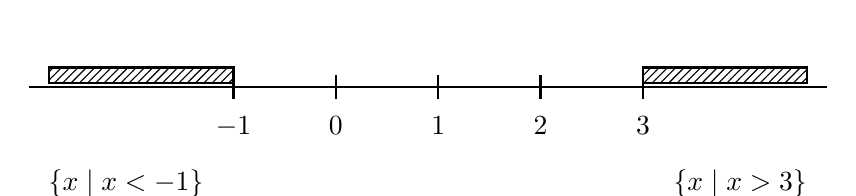
\begin{tikzpicture}[x=1.3cm, y=1cm]
    % Axis
    \draw[thick] (-3, 0) -- (4.8, 0);
    \foreach \x in {-1, 0, 1, 2, 3} {
        \draw[thick] (\x, 0.15) -- (\x, -0.15);
        \node[below=3pt] at (\x, -0.15) {$\x$};
    }

    % Shaded/hatched regions
    % x < -1
    \fill[pattern=north east lines, pattern color=black] (-2.8, 0.05) rectangle (-1, 0.25);
    \draw[thick] (-2.8, 0.05) rectangle (-1, 0.25);
    \node[below=22pt] at (-2.05, -0.15) {$\{x \mid x < -1\}$};

    % x > 3
    \fill[pattern=north east lines, pattern color=black] (3, 0.05) rectangle (4.6, 0.25);
    \draw[thick] (3, 0.05) rectangle (4.6, 0.25);
    \node[below=22pt] at (3.95, -0.15) {$\{x \mid x > 3\}$};
\end{tikzpicture}
\end{figure}

故（上）式的解是：$\{x \mid -1<x<3\}\cup\phi = \{x \mid -1<x<3\}$。

換句話說，坐標滿足原不等式的點在下圖所示 $A, B$ 間的點集內。

\begin{figure}[H]
\centering
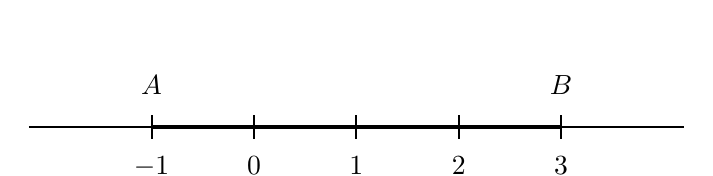
\begin{tikzpicture}[x=1.3cm, y=1cm]
    % Axis
    \draw[thick] (-2.2, 0) -- (4.2, 0);
    \foreach \x in {-1, 0, 1, 2, 3} {
        \draw[thick] (\x, 0.15) -- (\x, -0.15);
        \node[below=3pt] at (\x, -0.15) {$\x$};
    }

    % Segment AB
    \draw[ultra thick] (-1, 0) -- (3, 0);
    \node[above=4pt] at (-1, 0.15) {$A$};
    \node[above=4pt] at (3, 0.15) {$B$};
\end{tikzpicture}
\end{figure}

\begin{example}\label{ex:b2_2-3-3}
求直線上的點集，其坐標滿足下列不等式：
\[
f(x)=(x+1)(x-1)(x-3)>0.
\]
\end{example}
\paragraph{【解】} 由符號定則，我們可以把上述不等方歸於
\[
x+1,\quad x-1,\quad x-3.
\]
這三個因子各種可能的正、負組合的討論。同學們容易看出 $-1,\ +1,\ +3$ 分別是 $x+1,\ x-1$ 和 $x-3$ 這三個因子正、負的分界線。今列表如下：

\begin{figure}[H]
\centering
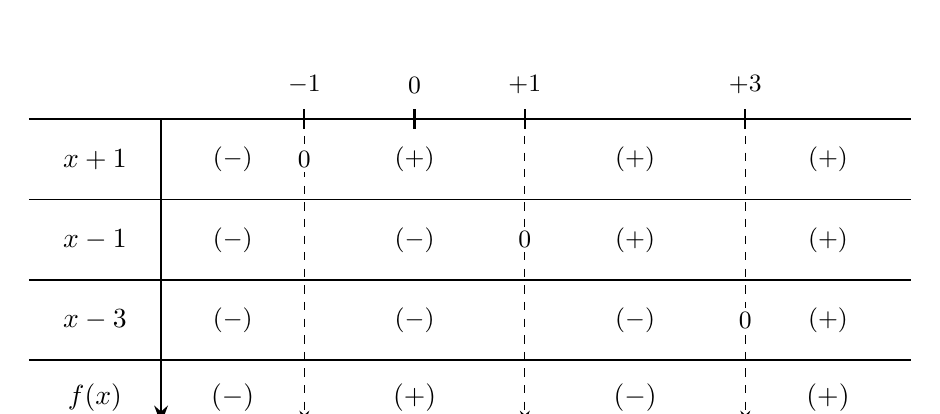
\begin{tikzpicture}[x=1.4cm, y=0.85cm, >=Stealth]
    % Top number line
    \draw[thick] (-3.5, 3.5) -- (4.5, 3.5);
    \foreach \x/\lbl in {-1/-1, 0/0, 1/+1, 3/+3} {
        \draw[thick] (\x, 3.65) -- (\x, 3.35);
        \node[above=2pt, font=\small] at (\x, 3.65) {$\lbl$};
    }

    % Vertical boundary lines (dashed down to f(x) row with downward ticks/arrows)
    \draw[dashed, ->] (-1, 3.5) -- (-1, -1.05);
    \draw[dashed, ->] (1, 3.5) -- (1, -1.05);
    \draw[dashed, ->] (3, 3.5) -- (3, -1.05);

    % Left border line (widened left column so x < -1 has ample room)
    \draw[thick, ->] (-2.3, 3.5) -- (-2.3, -1.05);

    % Horizontal grid lines
    \draw[thin] (-3.5, 2.3) -- (4.5, 2.3);
    \draw[thin] (-3.5, 1.1) -- (4.5, 1.1);
    \draw[thick] (-3.5, -0.1) -- (4.5, -0.1);

    % Row 1: x+1
    \node at (-2.9, 2.9) {$x+1$};
    \node at (-1.65, 2.9) {\small $(-)$};
    \node[fill=white, inner sep=1.5pt] at (-1, 2.9) {\small $0$};
    \node at (0, 2.9) {\small $(+)$};
    \node at (2, 2.9) {\small $(+)$};
    \node at (3.75, 2.9) {\small $(+)$};

    % Row 2: x-1
    \node at (-2.9, 1.7) {$x-1$};
    \node at (-1.65, 1.7) {\small $(-)$};
    \node at (0, 1.7) {\small $(-)$};
    \node[fill=white, inner sep=1.5pt] at (1, 1.7) {\small $0$};
    \node at (2, 1.7) {\small $(+)$};
    \node at (3.75, 1.7) {\small $(+)$};

    % Row 3: x-3
    \node at (-2.9, 0.5) {$x-3$};
    \node at (-1.65, 0.5) {\small $(-)$};
    \node at (0, 0.5) {\small $(-)$};
    \node at (2, 0.5) {\small $(-)$};
    \node[fill=white, inner sep=1.5pt] at (3, 0.5) {\small $0$};
    \node at (3.75, 0.5) {\small $(+)$};

    % Row 4: f(x)
    \node at (-2.9, -0.65) {$f(x)$};
    \node at (-1.65, -0.65) {$(-)$};
    \node at (0, -0.65) {$(+)$};
    \node at (2, -0.65) {$(-)$};
    \node at (3.75, -0.65) {$(+)$};
\end{tikzpicture}
\end{figure}

由上述表格，我們可以一目瞭然地看出 $f(x)>0$ 的解是
\[
-1x<1\text{，及 } x>3.\phantomsection\label{note:b2-ch2-p37-ex3-typo}
\]

\begin{example}\label{ex:b2_2-3-4}
求解 $2x^2-6x+25<0$。
\end{example}
\paragraph{【解】} 由於二次式 $2x^2-6x+25$ 的判別式
\[
\delta = (-6)^2 - 4\cdot 2\cdot 25 = -164 < 0,
\]
故由第一章的定理 3 的推論得知 $2x^2-6x+25$ 永遠為正，所以無解。

（同理：$2x^2-6x+25>0$ 的解是全部實數的集合）

\begin{example}\label{ex:b2_2-3-5}
求解不等式
\[
(2x^2-6x+25)(x+1)(x-1)(x-3)\le 0.
\]
\end{example}
\paragraph{【解】} 由〔例 4〕的討論，$2x^2-6x+25$ 永遠是正的，所以
\begin{align*}
&(2x^2-6x+25)(x+1)(x-1)(x-3)\le 0, \\
&\Updownarrow \\
&(x+1)(x-1)(x-3)\le 0.
\end{align*}
仿照〔例 3〕的辦法列表解得
\[
x\le -1\text{，及 } 1\le x\le 3.
\]
（同理：$(-2x^2+6x-25)g(x)\ge 0$ 和 $g(x)\le 0$ 有同解，因為 $-2x^2+6x-25$ 永遠是負的。）

\begin{example}\label{ex:b2_2-3-6}
求解不等式
\[
f(x) = \frac{x+1}{(x-1)(x-3)} > 0.
\]
\end{example}
\paragraph{【解】} 我們知道 $f(x)>0$ 的條件是要負的因子是偶數個，組成這個 $f(x)$ 的因子是 $x+1,\ x-1,\ x-3$，與〔例 3〕沒有什麼不一樣（只是 $x-1,\ x-3$ 被移到分母上罷了！）所以正負界限的討論，當然也應跟〔例 3〕相同。那麼，什麼是 $f(x)>0$ 的解呢？自然也是：$-1<x<1,\ x>3$。

\subsubsection*{習題 2-3}

\begin{enumerate}
    \item 試以圖表示下列各組不等式的界限：
    \begin{enumerate}[(i)]
        \item $\begin{cases} x>-1 \\ x>2 \end{cases}$
        \item $\begin{cases} x>5 \\ x<7 \end{cases}$
        \item $\begin{cases} x<0 \\ x\le 2 \end{cases}$
        \item $\begin{cases} -1\le x\le 1 \\ x\ge -2 \\ -5<x<9 \end{cases}$
    \end{enumerate}

    \item 在直線上分別描出坐標，滿足下列不等式的點集：
    \begin{enumerate}[(i)]
        \item $\frac{x}{x+1}<0$。
        \item $\frac{(x-1)^2}{2x-1}<0$。
        \item $\frac{(x+1)(x+2)}{x+3}>0$。
        \item $\frac{x+1}{(x-1)(x-3)}\ge 0$。
    \end{enumerate}

    \item 分別求出直線上的點集，其坐標滿足下列不等式：
    \begin{enumerate}[(i)]
        \item $2x^2+4x>x^2+6x+8$。
        \item $(x+1)(x-3)(x-4)\le 0$。
        \item $|x-1|<3$。
        \item $x^2+2x+5>0$。
        \item $1<|3x+2|\le 7$。
    \end{enumerate}

    \item 試解下列不等式：
    \begin{enumerate}[(i)]
        \item $\frac{x^2-7x+12}{x^2-3x+2} < -1$。
        \item $\frac{4x^2-20x+18}{x^2-5x+4} < 3$。
        \item $\frac{1}{x+1}+\frac{1}{x+4} > \frac{1}{x+3}+\frac{1}{x+2}$。
    \end{enumerate}

    \item 證明
    \begin{enumerate}[(i)]
        \item 不等式 $1+x+x^2>0$ 對於所有實數 $x$ 都成立，一般地，不等式 $1+x+x^2+\dots+x^{2n}>0$ ($n$ 是自然數) 對於所有實數也都成立。
        \item 方程式 $x^{2n+1}-1=0$ 祗有一個實根 ($=1$)。
    \end{enumerate}
\end{enumerate}

\subsection{數列的觀念與例子}\label{sec:b2_2-4}

首先，讓我們再來看看我們在數學領域中最先認識的老朋友——自然數。
\[
1, 2, 3, 4, 5, \dots, n, n+1, n+2, \dots.
\]
他們是一串依次排列的數，從 1 開始，逐次加以 1 至無窮。這就是本節要向大家介紹的數列（sequence）的一個原始的例子。在正式定義數列之前，讓我們再來舉幾個數列的例子。

\begin{example}\label{ex:b2_2-4-1}
假如你從今天開始每天儲蓄 10 元，則第一天你儲了 10 元，第二天你共儲了 20 元，以此類推，到第 $n$ 天共儲有 $10\cdot n$ 元。所以，你在各天儲蓄的累積總額可寫成下述數列。
\[
10, 20, 30, 40, \dots, n\cdot 10, (n+1)\cdot 10 \dots\dots
\]
\end{example}

\begin{example}\label{ex:b2_2-4-2}
假如你不但每天儲蓄 10 元，而且每儲滿 100 元時，就存入銀行，因而多得千分之一的日利（假設用單利法），那麼你每天的儲蓄累積總額就是下述數列：
\[
10, 20, 30, \dots, 90, 100;\ 110.1, 120.2, \dots, 201;\ 211.2, 221.4, \dots, 303;\ \dots
\]
以此類推，請同學試求上述數列的第 $365, 730, 1096, 1461$ 項。
\end{example}

\subsubsection*{4-1 數列的定義}

一個數列就是一串（如自然數一般）依次排列的數。

\begin{example}\label{ex:b2_2-4-3}
\leavevmode
\begin{enumerate}[(i)]
    \item $1, -1, 1, -1, \dots, (-1)^n, \dots$ 為一數列，其第 $n+1$ 項為 $(-1)^n$。
    \item $1, 0, -1, 0, 1, 0, -1, \dots$ 為一數列，其偶數項為 0，第 $4k+1$ 項為 1，第 $4k+3$ 項為 $-1$。
    \item $1, 4, 9, 16, \dots, n^2, \dots$ 為一數列，其第 $n$ 項為 $n^2$。
    \item $2, 3, 5, 7, 11, 13, \dots$, 第 $n$ 個質數, $\dots$ 為一數列，（因為在第一冊第六章中證明質數個數無窮。）
    \item $1, -1, 3, 7, 0, 0, \dots, 0, \dots$ 為一數列它的前四項為 $1, -1, 3, 7$，而自第五項起，皆為 0.
    \item $0, 0, 1, 0, 0, -1;\ 0, 0, 2, 0, 0, -2, \dots;\ 0, 0, n, 0, 0, -n+1, 0, 0, -(n+1), \dots$\phantomsection\label{note:b2-ch2-p40-ex3-vi} 為一數列，其第 $6n$ 項為 $-n$，第 $6n-3$ 項為 $n$，其他各項為零。
    \item $1, \frac{1}{2}, \frac{1}{3}, \frac{1}{4}, \dots, \frac{1}{n}, \dots$ 是第 $n$ 項為 $\frac{1}{n}$ 的數列。
    \item $a, a^2, a^3, \dots, a^n, \dots$ 是第 $n$ 項為 $a^n$ 的數列。
    \item $1, 4, 1, 5, 9, 2, 6, \dots$, （第 $n$ 項是 $\pi=3.1415926\dots$ 小數點線下的第 $n$ 位數字）。
\end{enumerate}
\end{example}

\subsubsection*{4-2 關於數列的符號用法}

在今後對於數列的討論中，我們將用 $a_n, b_n$ 或 $S_n, \dots$ 等符號表示某給定數列的第 $n$ 項（亦即用足標去標明第幾項）。用符號
\[
\langle a_n \mid n=1, 2, 3, \dots \rangle \quad (\text{或簡寫成 } \langle a_n \rangle)
\]
去表示第 $n$ 項為 $a_n$ 的數列。例如：$\langle (-1)^n \mid n=1, 2, 3, \dots \rangle$ 就是數列 $-1, +1, -1, +1, \dots$,
\[
\langle \frac{1}{1+n^2} \rangle \text{ 就是數列 } \frac{1}{2}, \frac{1}{5}, \frac{1}{10}, \frac{1}{17}, \dots
\]

\subsubsection*{4-3 數列的種類及其定義}

我們常見的數列例子有等差數列與等比數列

\begin{definition*}
等差數列 $\langle a_n \rangle$ 就是滿足 $a_2-a_1 = a_3-a_2 = a_n-a_{n-1} = \dots = d$ 的數列，$a_1$ 叫做首項，$d$ 叫做公差。
\end{definition*}

\begin{definition*}
等比數列（或幾何數列）$\langle b_n \rangle$ 就是滿足 $\frac{b_2}{b_1} = \frac{b_3}{b_2} = \dots = \frac{b_n}{b_{n-1}} = \dots = r$ 的數列（設各項 $\ne 0$）。 $b_1$ 叫做首項，$r$ 叫做公比。
\end{definition*}

我們甚至可以用等差數列來做出一種新的數列：如果 $\langle a_n \rangle$ 為一等差數列，每一項 $a_n \ne 0$，我們就把 $a_n$ 的倒數所成的數列 $\langle \frac{1}{a_n} \rangle$ 叫做調和數列。也就是說我們有：

\begin{definition*}
調和數列 $\langle h_n \rangle$ 就是滿足
\[
\frac{1}{h_2}-\frac{1}{h_1} = \frac{1}{h_3}-\frac{1}{h_2} = \dots = \frac{1}{h_n}-\frac{1}{h_{n-1}}
\]
的數列。
\end{definition*}

顯然地，$\frac{2}{h_2} = \frac{1}{h_1}+\frac{1}{h_3} = \frac{h_1+h_3}{h_1 h_3}$， $2h_1 h_3 = h_2(h_1+h_3)$。

所以一般相連的項之間有下列關係：
\[
2h_{n-1}h_{n+1} = h_n(h_{n-1}+h_{n+1}).
\]

\subsubsection*{習題 2-4}

\begin{enumerate}
    \item 已知等比數列中兩項，求數列的前五項及一般項 $a_n$：
    \begin{enumerate}[(i)]
        \item $a_2=\frac{121}{100},\ a_4=\frac{1331}{1000}$。
        \item $b_2=6,\ b_5=48$。
        \item $c_6=18,\ c_9=54$。
        \item $d_4=\frac{4}{9},\ d_7=\frac{32}{243}$。
    \end{enumerate}

    \item 已知等差數列中某二項，求數列的前五項及一般項 $a_n$：
    \begin{enumerate}[(i)]
        \item $a_3=5,\ a_8=9$。
        \item $a_4=10,\ a_{11}=6$。
        \item $a_9=30$, 公差 $=-5$。
    \end{enumerate}

    \item 如果 $\langle a_n \rangle$ 是一個等比數列，證明 $\langle \frac{1}{a_n} \rangle$ 也是一個等比數列。

    \item 已知調和數列兩項，求前五項及一般項 $a_n$：
    \begin{enumerate}[(i)]
        \item 第三項是 3，第七項是 3.
        \item 第二項是 $\frac{1}{9}$，第十一項是 $\frac{1}{50}$。
    \end{enumerate}
\end{enumerate}

\subsection{極限的概念及基本性質}\label{sec:b2_2-5}

數列在數學中的重要性在於它是討論極限的基本工具。本節將對數列的極限及其基本性質作一初步介紹。在下一章中，我們將進一步用它來討論實數系的重要特性——完備性（或稱為連續性）。極限概念和實數系的完備性是往後微積分學的基礎，也是研究自然現象、工程問題、統計學等等所不可或缺的基本工具。

\subsubsection*{5-1 極限概念}

\begin{example}\label{ex:b2_2-5-1}
仔細觀察數列 $1, \frac{1}{2}, \frac{1}{3}, \frac{1}{4}, \dots, \frac{1}{n}, \dots$，我們馬上看出：
\begin{enumerate}[(i)]
    \item 上述數列的每項都是正數。
    \item 上述數列，逐項遞減：
    \[
    1 > \frac{1}{2} > \frac{1}{3} > \dots > \frac{1}{n} > \frac{1}{n+1} > \dots.
    \]
    \item 當 $n$ 愈來愈大時，第 $n$ 項 $\frac{1}{n}$ 不但愈來愈接近 0，而且要多近就能多近。這種情形，我們就說：數列 $\langle \frac{1}{n} \rangle$ 趨近 0，或收斂到 0，或 0 是數列 $\langle \frac{1}{n} \rangle$ 的極限，用記號
    \[
    \frac{1}{n}\to 0, \quad \text{或 } \lim_{n\to\infty}\frac{1}{n}=0, \quad \text{或 } \lim\frac{1}{n}=0 \text{ 表示}.
    \]
\end{enumerate}
\end{example}

現在讓我們再用直線坐標系，把上述事實圖解說明如下：

\begin{figure}[H]
\centering
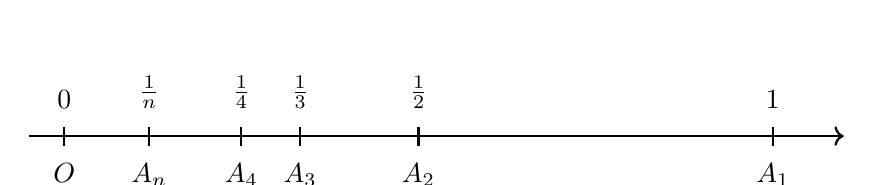
\begin{tikzpicture}[x=9cm, y=1cm]
    % Number line
    \draw[thick, ->] (-0.05, 0) -- (1.1, 0);

    % Ticks and coordinates
    % 0 (origin O)
    \draw[thick] (0, 0.12) -- (0, -0.12);
    \node[above=3pt] at (0, 0.12) {$0$};
    \node[below=3pt] at (0, -0.12) {$O$};

    % 1/n
    \draw[thick] (0.12, 0.12) -- (0.12, -0.12);
    \node[above=3pt] at (0.12, 0.12) {$\frac{1}{n}$};
    \node[below=3pt] at (0.12, -0.12) {$A_n$};

    % 1/4
    \draw[thick] (0.25, 0.12) -- (0.25, -0.12);
    \node[above=3pt] at (0.25, 0.12) {$\frac{1}{4}$};
    \node[below=3pt] at (0.25, -0.12) {$A_4$};

    % 1/3
    \draw[thick] (0.333, 0.12) -- (0.333, -0.12);
    \node[above=3pt] at (0.333, 0.12) {$\frac{1}{3}$};
    \node[below=3pt] at (0.333, -0.12) {$A_3$};

    % 1/2
    \draw[thick] (0.5, 0.12) -- (0.5, -0.12);
    \node[above=3pt] at (0.5, 0.12) {$\frac{1}{2}$};
    \node[below=3pt] at (0.5, -0.12) {$A_2$};

    % 1
    \draw[thick] (1.0, 0.12) -- (1.0, -0.12);
    \node[above=3pt] at (1.0, 0.12) {$1$};
    \node[below=3pt] at (1.0, -0.12) {$A_1$};
\end{tikzpicture}
\end{figure}

在直線上取以數列：
\[
1, \frac{1}{2}, \frac{1}{3}, \frac{1}{4}, \dots, \frac{1}{n}, \dots
\]
的各項為坐標的各點，就得到一個點列：
\[
A_1, A_2, A_3, \dots, A_n, \dots.
\]
上述點列 $\langle A_n \rangle$ 從原點 0 的右邊逐步向原點逼近：
\[
0 < \dots < A_{n+1} < A_n < \dots < A_3 < A_2 < A_1;
\]
而且可以逼近到隨心所欲的程度。

\begin{example}\label{ex:b2_2-5-2}
$\frac{1}{2}, \frac{2}{3}, \frac{3}{4}, \dots, \frac{n}{n+1}, \dots$
\end{example}
同學們可以容易看出這個數列逐項遞增，其第 $n$ 項 $a_n = \frac{n}{n+1}$ 永遠小於 1，但是當 $n$ 愈來愈大時，$a_n$ 和 1 的差異 $|a_n-1| = \frac{1}{n+1}$ 可以小到隨心所欲的小。換句話說，
\[
\frac{n}{n+1} \to 1.
\]

\begin{example}\label{ex:b2_2-5-3}
$(-\frac{1}{2}), (-\frac{1}{2})^2, (-\frac{1}{2})^3, (-\frac{1}{2})^4, \dots, (-\frac{1}{2})^n, \dots$
\end{example}
這個數列逐項正負相間，所以不再是遞減或遞增數列，但是其第 $n$ 項 $a_n$ 和 0 的差異 $|a_n-0| = |a_n| = (\frac{1}{2})^n$ 顯然可以小到隨心所欲的小。所以
\[
\lim\left(-\frac{1}{2}\right)^n = 0
\]

以上三個例子的數列，都有極限，這樣的數列叫做收斂數列。但是並不是每一個數列都收斂；不收斂的數列叫做發散數列。請看下例：

\begin{example}\label{ex:b2_2-5-4}
數列 $1, 4, 9, 16, \dots, n^2, \dots$ 顯然沒有極限。
\end{example}

\begin{example}\label{ex:b2_2-5-5}
數列 $+1, -1, +1, -1, +1, \dots$ 也不收斂。
\end{example}

\paragraph{註：} 例 4 的情形為發散至正無窮大，寫做 $n^2 \to \infty$。例 5 的情形叫做振動。當然還有其他發散的情形。例如數列 $1, -2, +3, -4, +5, \dots$。

\begin{example}\label{ex:b2_2-5-6}
級數 $1, r, r^2, r^3, r^4, \dots, r^n, \dots$\phantomsection\label{note:b2-ch2-p44-ex6-series-term} 的收斂與發散有下列幾種情形：
\begin{align*}
&\text{當 } r<1 \text{ 時 } \lim_{n\to\infty} r^n = 0\phantomsection\label{note:b2-ch2-p44-ex6-r-range} \\
&\text{當 } r=1 \text{ 時 } \lim_{n\to\infty} r^n = 1 \\
&\text{當 } r>1 \text{ 時 } \lim_{n\to\infty} r^n = \infty
\end{align*}
\end{example}

\subsubsection*{習題 2-5}

\begin{enumerate}
    \item 問下列數列是收斂？還是發散？
    \begin{enumerate}[(i)]
        \item $1, -0.2, 0.04, -0.008, \dots$, 第 $n$ 項為 $(\frac{-2}{10})^{n-1}$。
        \item $3, \frac{3}{2}, \frac{3}{4}, \frac{3}{8}, \dots$ 第 $n$ 項為 $\frac{3}{2^{n-1}}$。
        \item $10, \frac{10^2}{9}, \frac{10^3}{9^2}, \dots$, 第 $n$ 項為 $\frac{10^n}{9^{n-1}}$。
    \end{enumerate}

    \item 下列數列中那些是收斂？那些是發散到 $\infty$？
    \begin{enumerate}[(i)]
        \item $a_n = n^2$。
        \item $a_n = \frac{100\cdot n}{n^2}$。
        \item $a_n = \frac{n^2-1}{n+100}$。
        \item $a_n = \frac{1-n}{1+n}$。
        \item $a_n = (-1)^n n$。
    \end{enumerate}

    \item 證明
    \begin{enumerate}[(i)]
        \item 如果等差數列 $\langle a_n \rangle$ 的公差 $>0$，那麼 $\langle a_n \rangle$ 是遞增數列；反之如果公差 $<0$ 就是遞減數列。
        \item 如果等比數列 $\langle a_n \rangle$ 的公比 $r>1$，那麼 $\langle a_n \rangle$ 是遞增數列。反之如果 $0<r<1$ 就是遞減。
        \item 調和數列不是遞增就是遞減數列。
    \end{enumerate}
\end{enumerate}

\subsubsection*{5-2 極限的基本性質}

如果兩個數列 $\langle a_n \rangle$、$\langle b_n \rangle$ 都收斂，那麼它們的和數列 $\langle a_n+b_n \rangle$、差數列 $\langle a_n-b_n \rangle$、積數列 $\langle a_n b_n \rangle$ 也都收斂，而且有
\begin{enumerate}[(i)]
    \item $\lim(a_n+b_n) = \lim a_n + \lim b_n$。
    \item $\lim(a_n-b_n) = \lim a_n - \lim b_n$。
    \item $\lim a_n b_n = \lim a_n \cdot \lim b_n$。
\end{enumerate}

\begin{example}\label{ex:b2_2-5-7}
常數數列 $c, c, c, \dots, c, \dots$ 當然收斂到 $c$。
\end{example}

\begin{example}\label{ex:b2_2-5-8}
由例 7 及性質 (iii) 就得：如果 $\langle a_n \rangle$ 收斂，那麼
\[
\lim c a_n = c \lim a_n.
\]
\end{example}

轉到商數列 $\langle \frac{a_n}{b_n} \rangle$ 的討論，大家當然要問：如果數列 $\langle a_n \rangle$，$\langle b_n \rangle$ 收斂，是不是商數列 $\langle \frac{a_n}{b_n} \rangle$ 也收斂？收斂到 $\frac{\lim a_n}{\lim b_n}$？

當然 $b_n$ 都不能等於 0，不然的話商數列 $\langle \frac{a_n}{b_n} \rangle$ 就沒有意義，同樣的道理 $\lim b_n$ 也不能是 0，不然的話 $\frac{\lim a_n}{\lim b_n}$ 也沒有意義。事實上，這個必要條件也是充分條件。

如果 $\langle a_n \rangle$，$\langle b_n \rangle$ 都收斂，而且 $b_n$ 都不等於 0，以及 $\lim b_n \ne 0$，那麼商數列 $\langle \frac{a_n}{b_n} \rangle$ 收斂，而且
\begin{enumerate}[(iv)]
    \item $\lim\frac{a_n}{b_n} = \frac{\lim a_n}{\lim b_n}$。
\end{enumerate}

\begin{example}\label{ex:b2_2-5-9}
數列 $\langle \frac{1}{n^2} \rangle$，$\langle \frac{1}{n} \rangle$ 都收斂到 0，但商數列
\[
\langle \frac{\frac{1}{n^2}}{\frac{1}{n}} \rangle = \langle \frac{1}{n} \rangle \text{ 收斂到 0，但 } \langle \frac{\frac{1}{n}}{\frac{1}{n^2}} \rangle = \langle n \rangle \text{ 發散到無窮大}.
\]
所以 $\lim b_n = 0$ 時，商數列 $\langle \frac{a_n}{b_n} \rangle$ 可能收斂也可能發散。
\end{example}

\subsubsection*{習題 2-6}

\begin{enumerate}
    \item 求下列各數列之極限：
    \begin{enumerate}[(i)]
        \item $\overbrace{0, 0, 0, 0, \dots, 0}^{1000\text{項}}, 1, 1, 1, \dots, 1, \dots$ （即前 1000 項都是 0，以後都是 1）。
        \item $0, 0, 0, 0, \dots, 0\dots$ （每一項都是 0）。
        \item $(6+\frac{1}{n})(\frac{n+2}{2n+1}-1)$。
        \item $(\frac{2n^2-3}{3n^2-2})^2$。
        \item $\frac{n^2+n+1}{\frac{n^2+3}{n+1}}$。
        \item $3n(\frac{2}{n}+\frac{2n^2+9}{n^3+n+1.5})$。
        \item $\frac{2n^2(n-3+4n^2)}{5(n-1)^3(3n+4)}$。
    \end{enumerate}

    \item 設 $a_n = \frac{2n+1}{n^2},\ b_n = \frac{1-n^2}{3+n-n^2},\ c_n = \frac{n^3}{1-n}$，求下列各數列之極限：
    \[
    \langle a_n \rangle,\quad \langle b_n \rangle,\quad \langle c_n \rangle,\quad \langle a_n+c_n \rangle,\quad \langle b_n c_n \rangle,\quad \langle \frac{a_n}{c_n} \rangle,\quad \langle \frac{c_n}{a_n} \rangle,
    \]
    \[
    \langle -\frac{b_n}{c_n} \rangle,\quad \langle \frac{b_n}{a_n} \rangle,\quad \langle 3a_n - \frac{1}{2}b_n \rangle,\quad \langle \frac{4b_n}{a_n+c_n} \rangle.
    \]

    \item 求下列各極限：
    \begin{enumerate}[(i)]
        \item $\lim_{n\to\infty}(\frac{n^2-n}{n+1}-\frac{n^2+n}{n-1})$。
        \item $\lim_{n\to\infty}(\frac{101}{100})^n$。
        \item $\lim_{n\to\infty}(\frac{99}{100})^n$。
    \end{enumerate}
\end{enumerate}

\subsection{無窮級數和循環小數}\label{sec:b2_2-6}

小學和中學都教過：循環小數
\[
0.6666\dots = \frac{2}{3}.
\]
在這一節中我們要仔細思考它的意思，證明每個循環小數都等於一個分數，而每個分數都等於一個循環小數。

\subsubsection*{6-1 無限小數}

從整數因子分解的唯一性，我們得知：一個不可約分數 $\frac{p}{q}$ ($p, q$ 互質) 能表成一個有限位小數的必要充分條件是 $q$ 只含有 2 或 5 這兩種質因子。譬如 $\frac{2}{3}, \frac{5}{7}$ 等分數不能表成有限小數。今以 $\frac{2}{3}$ 為例，作下述分析：

\begin{enumerate}[(i)]
    \item 以 3 去除 2，得
    \[
    \begin{array}{r@{\quad}l}
        & 0.666\dots \\
        \cline{2-2}
        3 & )\, 2000\dots \\
        & \phantom{)\, 1} 18 \\
        \cline{2-2}
        & \phantom{)\, 0} 20 \\
        & \phantom{)\, 0} 18 \\
        \cline{2-2}
        & \phantom{)\, 00} 20 \\
        & \phantom{)\, 00} 18 \\
        \cline{2-2}
        & \phantom{)\, 000} 2
    \end{array}
    \]

    \item 上述除式的意義是：
    \begin{align*}
    2 = 0.6\times 3 + 0.2 &\iff 0.6 < \frac{2}{3} < 0.7, \\
    = 0.66\times 3 + 0.02 &\iff 0.66 < \frac{2}{3} < 0.67, \\
    = 0.666\times 3 + 0.002 &\iff 0.666 < \frac{2}{3} < 0.667, \\
    &\dots\dots\dots\dots\dots\dots\dots
    \end{align*}
\end{enumerate}

從上面的分析，同學們可以看出 $\frac{2}{3}$ 雖然不能用有限位小數表出，但是存在着由有限位小數所成的數列：
\[
a_1 = 0.6,\quad a_2 = 0.66,\quad a_3 = 0.666\dots,\quad a_n = \underbrace{0.666\dots 66}_{n\text{ 位小數}}
\]
上述數列和 $\frac{2}{3}$ 的關係是
\[
a_n = \underbrace{0.666\dots 66}_{n\text{ 位}} < \frac{2}{3} < \underbrace{0.666\dots 67}_{n\text{ 位}} = a_n + \frac{1}{10^n}.
\]
換句話說，$a_n$ 和 $\frac{2}{3}$ 之間的差異小於 $\frac{1}{10^n}$，這個差異當 $n$ 越來越大時，當然會任意地小。所以
\[
a_n \to \frac{2}{3}
\]
我們通常寫 $0.666\dots = \frac{2}{3}$ 的意思就是這樣：如果
\[
a_n = \underbrace{0.666\dots 66}_{n\text{ 位}},
\]
那麼
\[
a_n \to \frac{2}{3}.
\]
同樣地，我們寫 $\pi = 3.1415926\dots$ 時，我們的意思是：

令 $a_1=3.1,\ a_2=3.14,\ a_3=3.141,\ a_4=3.1415,\ \dots$

那麼 $a_n \to \pi$。

若把 \hyperref[sec:b2_2-4]{§ 4}〔例 3〕之 (ix) 的數列寫做 $c_n$，那麼
\[
a_n = 3 + \sum_{k=1}^n \frac{c_k}{10^k}.
\]
所以無限小數的解釋是這個樣子：我們取它小數點以下第 $n$ 位為止的有限小數，記做 $a_n$，那麼數列 $a_n$ 的極限就等於這個無限小數。

讓我們回憶一下從前怎樣證明 $0.6666\dots = \frac{2}{3}$，根據以上的解釋，這個式子表示 $a_n \to \frac{2}{3}$，其中
\[
a_n = \underbrace{0.666\dots 66}_{n\text{ 位}}.
\]
我們說：因為
\[
a = 0.666\dots
\]
所以
\[
10a = 6.666\dots
\]
所以
\[
9a = 10a-a = 6,\quad \text{即 } a = \frac{6}{9} = \frac{2}{3}.
\]
這個論證其實稍微有點問題：因為你必須先假定 $a=0.666\dots$ 這個數的存在（也就是說 $a_n$ 收斂）。這一點參看下一章，不過我們有另一個辦法，不需這個假定。

我們看出 $a_n$ 和 $a_{n-1}$ 的差是 $\underbrace{0.000\dots 0}_{n\text{ 位}}6$。這個差越來越小，而且“每步就小 10 倍”. 換句話說
\begin{align*}
a_1 &= 0.6 = b_1; \\
a_2 &= 0.6+0.06 = b_1+b_2,\quad \text{其中 } b_2 = b_1 \frac{1}{10}; \\
a_3 &= 0.6+0.06+0.006 = b_1+b_2+b_3,\quad \text{其中 } b_3 = b_2 \frac{1}{10};
\end{align*}
依此類推，而有
\[
a_n = b_1+b_2+b_3+\dots+b_n,
\]
其中 $b_1 = 0.6$，而 $b_n = b_1 r^{n-1},\ r = \frac{1}{10}$。

當我們看差額 $a_n - a_{n-1} = b_n$ 時，我們就有一個無窮等比數列 $\langle b_n \rangle$。 $a_n$ 是這數列的首 $n$ 項和。而我們想去證明的也就是
\[
b_1+b_2+b_3+\dots = \frac{2}{3}.
\]
(即 $\sum_{i=1}^n b_i \to \frac{2}{3}$)

我們利用眾所週知的公式：
\[
(1-r)(1+r+r^2+\dots+r^{k-1}) = 1-r^k
\]
因此當 $r\ne 1$ 時，有
\[
1+r+r^2+\dots+r^{k-1} = \frac{1-r^k}{1-r}.
\]
可以知道
\begin{equation}\label{eq:b2_ch2_geom_sum}\tag{1}
b_1+b_1 r+b_1 r^2+\dots+b_1 r^{n-1} = b_1 \frac{1-r^n}{1-r} = \frac{b_1}{1-r} + \frac{-r^n}{1-r}
\end{equation}
\phantomsection\label{note:b2-ch2-p50-eq1-b1}

在我們的例子，$|r|<1$，因此由（5-1）〔例 6〕$\frac{-r^n}{1-r} \to 0$\phantomsection\label{note:b2-ch2-p51-lim-rn}，所以
\[
a_n = b_1+b_1 r+b_1 r^2+\dots+b_1 r^{n-1} \to \frac{b_1}{1-r}, \quad (|r|<1).
\]
我們就寫成
\begin{equation}\label{eq:b2_ch2_geom_series_23}\tag{2}
\frac{2}{3} = \sum_{i=0}^\infty b_1 r^i = \frac{b_1}{1-r},\quad (|r|<1)
\end{equation}
的形式。

\subsubsection*{6-2 無窮級數}

上面的證明也提示了一些新的概念：（無窮）級數。

一般的來說，如果 $\langle b_n \rangle$ 是個數列，那麼我們用記號
\[
b_1+b_2+b_3+\dots \quad \text{或} \quad \sum_{i=1}^\infty b_i
\]
表示一個級數。

我們把首 $n$ 項的和
\[
a_n = b_1+b_2+\dots+b_n
\]
叫做第 $n$ 個部分和。這種部分和所成的數列 $\langle a_n \rangle$ 如果收斂，那麼我們說這級數 $\sum_{n=1}^\infty b_n$ 收斂，並且把 $\lim_{n\to\infty} a_n$ 叫做這級數的和。而記做
\[
\sum_{n=1}^\infty b_n = \lim_{n\to\infty} a_n.
\]
反之，如果 $\langle a_n \rangle$ 發散，我們就說級數 $\sum_1^\infty b_n$ 發散。 $b_n$ 叫做級數 $\sum_1^\infty b_n$ 的第 $n$ 項，而當數列 $\langle b_n \rangle$ 是等比數列時，級數 $\sum_1^\infty b_n$ 叫等比級數。

數列 $\langle b_n \rangle$ 的公比就是級數 $\sum_1^\infty b_n$ 的公比。為了討論循環小數及下一章的需要，讓我們來看看下面兩個定理：

\begin{theorem}\label{thm:b2_2-6-1}
如果 $\sum_{n=1}^\infty b_n$ 是等比級數，那麼它收斂的充分必要條件是公比 $r$ 的絕對值小於 1，此時它的和是 $\frac{b_1}{1-r}$。
\end{theorem}
\paragraph{【證明】} 充分性，從 (1)、(2) 兩式馬上知道，要證明必要性，我們只須注意到，如果 $|r| \ge 1$，那麼 $b_n = b_1 r^{n-1}$ 不會趨近于 0，但我們顯然有下列定理

\begin{theorem}\label{thm:b2_2-6-2}
如果數列 $\langle a_n \rangle$ 收斂，那麼 $a_n - a_{n-1}$ 收斂到 0. 因此，如果級數 $\sum_{n=1}^\infty b_n$ 收斂，那麼 $b_n \to 0$，因為第 $n$ 部分和是 $a_n = \sum_{i=1}^n b_i$，所以 $a_n - a_{n-1} = b_n \to 0$。
\end{theorem}

\begin{example}\label{ex:b2_2-6-1}
$\frac{1}{1}+\frac{1}{2}+\frac{1}{3}+\dots+\frac{1}{n}+\dots$ 是發散級數。為什麼呢？我們首先注意到這是正項級數，因此，部分和會越來越大。而且
\begin{align*}
a_1 &= 1, \\
a_2 &= 1+\frac{1}{2}, \\
a_4 &= 1+\frac{1}{2}+\frac{1}{3}+\frac{1}{4} > 1+\frac{1}{2}+\frac{1}{4}+\frac{1}{4} = 1+\frac{1}{2}+\frac{1}{2}, \\
a_8 &= 1+\frac{1}{2}+\frac{1}{3}+\frac{1}{4}+\frac{1}{5}+\frac{1}{6}+\frac{1}{7}+\frac{1}{8} \\
&> 1+\frac{1}{2}+\frac{1}{4}+\frac{1}{4}+\frac{1}{8}+\frac{1}{8}+\frac{1}{8}+\frac{1}{8} = 1+\frac{1}{2}+\frac{1}{2}+\frac{1}{2}.
\end{align*}
一般地
\[
a_{2^m} > 1 + \underbrace{\frac{1}{2}+\frac{1}{2}+\dots+\frac{1}{2}}_{m\text{ 個}} = \frac{m+2}{2}
\]
因 $a_{2^m}$ 越來越大毫無止境！所以 $a_n$ 只有發散到無限大。

注意到：$b_n = \frac{1}{n} \to 0$。因此，定理 2 中的 $b_n \to 0$ 是 $\sum b_n$ 收斂的必要條件，但並非充分條件。
\end{example}

\subsubsection*{習題 2-7}

\begin{enumerate}
    \item 求級數的和：
    \begin{enumerate}[(i)]
        \item $1 - \frac{1}{2} + \frac{1}{4} - \dots + (-\frac{1}{2})^{n-1} + \dots$。
        \item $\frac{1}{1\cdot 2} + \frac{1}{2\cdot 3} + \frac{1}{3\cdot 4} + \dots + \frac{1}{n\cdot(n+1)} + \dots$。
        
        （提示：$\frac{1}{n(n+1)} = \frac{1}{n} - \frac{1}{n+1}$）
        \item $3 + \frac{3}{8} + \dots + \frac{3}{8^{n-1}} + \dots$。
    \end{enumerate}

    \item 設一等差數列 $\langle a_n \rangle$ 的公差是 $d$，寫出其第 $n$ 項與前 $n$ 項和的公式。

    \item 有一等差數列 $\langle a_n \rangle$，首項 $a_1=3,\ a_{15}=-25$，求它的公差和前 15 項和。

    \item 證明無窮級數 $1 + \frac{1}{3} + \frac{1}{5} + \frac{1}{7} + \dots + \frac{1}{2n-1} + \dots$ 是發散的。

    \item 如果 $\langle a_n \rangle$ 是等差數列，證明級數
    \[
    a_1+a_2+\dots+a_n+\dots
    \]
    是發散級數。

    \item 已知級數的部分和，寫出各級數與它們的和：
    \begin{enumerate}[(i)]
        \item $S_n = \frac{1}{2^n}$。
        \item $S_n = 1 - \frac{1}{n}$。
        \item $S_n = \frac{7^{n-1}-1}{3\cdot 7^{n-2}}$。
    \end{enumerate}
\end{enumerate}

\subsubsection*{6-3 循環小數和分數}

下面定理 3 關於循環小數與分數間關係的證明，可能讀起來有些抽象。所以我們先用例子來說明一下。

\begin{example}\label{ex:b2_2-6-2}
試將 $0.3\overline{12}\ (=0.3121212\dots)$ 化為分數。
\end{example}
\paragraph{【解】} 
\begin{align*}
0.3\overline{12} &= \frac{3}{10}+\left(\frac{1}{10^2}+\frac{2}{10^3}\right)+\left(\frac{1}{10^4}+\frac{2}{10^5}\right)+\left(\frac{1}{10^6}+\frac{2}{10^7}\right)+\dots \\
&= \frac{3}{10}+\frac{12}{10^3}+\frac{12}{10^5}+\frac{12}{10^7}+\dots \\
&= \frac{3}{10}+\frac{12}{10^3}\left(1+\frac{1}{10^2}+\frac{1}{10^4}+\frac{1}{10^6}+\dots\right) \\
&= \frac{3}{10}+\frac{12}{10^3}\cdot\frac{1}{1-\frac{1}{10^2}} \\
&= \frac{3}{10}+\frac{12}{10^3}\cdot\frac{10^2}{99} \\
&= \frac{3}{10}+\frac{12}{990} \\
&= \frac{103}{330}.
\end{align*}
當我們仔細看這個例子，可以知道所以能夠將這個極限（也就是這個分數）找出來，是因為將第一個循環部分（就是 $\frac{12}{10^3}=0.012$）提出來後，在括弧內的級數是 $1+\frac{1}{10^2}+\frac{1}{10^4}+\dots+\frac{1}{10^{2n}}+\dots$ 這樣的等比級數。它們的公比是 $\frac{1}{100}(<1)$，所以有極限 $\frac{100}{99}$，而由這個極限就可以逐步算出整個循環小數的極限了。

\begin{example}\label{ex:b2_2-6-3}
試將 $\frac{8}{33}$ 化為小數。
\end{example}
\paragraph{【解】} 利用除法：
\[
\begin{array}{r@{\quad}ll}
    & 0.242424\dots & \\
    \cline{2-2}
    33 & )\, 80 & \\
    & \phantom{)\, } 66 & \\
    \cline{2-2}
    & \phantom{)\, } 140 & \left.\vphantom{\begin{array}{c}1\\1\end{array}}\right\} * \\
    & \phantom{)\, } 132 & \\
    \cline{2-2}
    & \phantom{)\, 0} 80 & \\
    & \phantom{)\, 0} 66 & \\
    \cline{2-2}
\end{array}
\]

我們由上面的除式看出，所以能每隔兩位就重複的緣故是 $*$ 部分相減後剩餘為 8，而開始也是 8，既然除數不變，那麼一切過程會再來一次，這樣一次一次的重複，就成了循環小數。

如果 $a$ 是個循環小數，它的循環節是由第 $k+1$ 位開始，到 $k+l$ 位。平常我們寫做
\[
a = a_0.c_1 c_2 \dots c_k \overline{c_{k+1} c_{k+2} \dots c_{k+l}}.
\]
($c_i$ 及 $a_0$ 是整數，而 $0\le c_i < 10,\ 0\le a_0$)

它的意思就是
\begin{align*}
a = a_0 &+ \frac{c_1}{10} + \frac{c_2}{10^2} + \dots + \frac{c_k}{10^k} + \frac{c_{k+1}}{10^{k+1}} + \dots + \frac{c_{k+l}}{10^{k+l}} \\
&+ \frac{c_{k+1}}{10^{k+l+1}} + \frac{c_{k+2}}{10^{k+l+2}} + \dots + \frac{c_{k+l}}{10^{k+2l}} + \frac{c_{k+1}}{10^{k+2l+1}} + \dots
\end{align*}
顯然的，這不是個等比級數。

第 $k$ 個部分和是分數
\[
a_k = a_0 + \frac{c_1}{10^1} + \frac{c_2}{10^2} + \dots + \frac{c_k}{10^k}.
\]
如果我們令
\[
d \equiv \frac{c_{k+1}}{10^{k+1}} + \frac{c_{k+2}}{10^{k+2}} + \frac{c_{k+3}}{10^{k+3}} + \dots + \frac{c_{k+l}}{10^{k+l}}
\]
（所以 $d$ 是分數而且 $0\le d < 1$）。那麼第 $k+ml$ 個部分和是\phantomsection\label{note:b2-ch2-p56-partial-sum-r}
\begin{align*}
a_{k+ml} &= a_k + d + d\frac{1}{10^l} + d\frac{1}{10^{2l}} + \dots + d\frac{1}{10^{(m-1)l}} \\
&= a_k + d\left(1+r+r^2+\dots+\frac{1}{r^{m-1}}\right)
\end{align*}
其中 $r = \frac{1}{10^l}$。所以
\[
a' = \lim_{m\to\infty} a_{k+ml} = a_k + \frac{d}{1-r} = a_k + \frac{10^l d}{10^l - 1} \text{ 是分數}.
\]
我們只證明了部分和數列的“子數列” $\langle a_{k+ml} \mid m=1, 2, \dots \rangle$ 收斂到分數 $a'$，要怎麼證明 $\langle a_n \rangle$ 也收斂到 $a$ 呢？

我們只須注意到原來的循環小數所代表的無窮級數也都是正項的，這就是說，部分和數列 $\langle a_n \rangle$ 是遞增數列。特別地，如果 $k+ml \le n < k+(m+1)l$，那麼 $a_{k+ml} \le a_n \le a_{k+(m+1)l}$。因此，如果“子數列” $\langle a_{k+ml} \mid m=1, 2, \dots \rangle$ 收斂到 $a'$，原數列 $\langle a_n \rangle$ 也收斂到 $a'$。

我們已證明了：每個循環小數都可化為分數，現在再證分數可以化為循環小數。

設 $\frac{m}{n}$ 為一任意給定的不可約分數（亦即 $m, n$ 互質），若 $q$ 上含有 2 或 5 的質因子\phantomsection\label{note:b2-ch2-p56-q-typo}，則容易看出 $\frac{m}{n}$ 可以化成有限位小數，我們可以把有限位小數看成循環小數的特例。（如 $\frac{1237}{2\times 5^3} = \frac{1237\times 2^2}{10^3} = 4.948 = 4.948\overline{0} = 4.947\overline{9}$。）反之，若 $n$ 含有不是 2 或 5 的質因子，則 $\frac{m}{n}$ 不可能寫成 $\frac{m'}{10^k}$ 的形式。（證明：整數因子分解的唯一性。）故 $\frac{m}{n}$ 不可能化為有限位小數。
\begin{align*}
m &= q_0 n + r_0 & 0 &< r_0 < n \\
10r_0 &= q_1 n + r_1 & 0 &< r_1 < n \\
10r_1 &= q_2 n + r_2 & 0 &< r_2 < n \\
&\vdots & &\vdots \\
10r_{n-1} &= q_n n + r_n & 0 &< r_n < n
\end{align*}
因為每一個 $r_i$ 都是大於 0 小於 $n$ 的正數，這種正數只有 $n-1$ 個。所以 $r_0, r_1, \dots, r_n$ 這 $n+1$ 個數必然有二者會相同，就假定這兩個相同的是 $r_k$ 和 $r_{k+l}$ 吧！

我們有：
\begin{align*}
10r_{k-1} &= q_k n + r_k \\
10r_k &= q_{k+1} n + r_{k+1} \\
&\vdots \\
10r_{k+l-1} &= q_{k+l} n + r_{k+l} \\
&= q_{k+l} n + r_k
\end{align*}
如果我們再做下去，應該又會有：
\begin{align*}
10r_k &= q_{k+1} n + r_{k+1} \\
&\vdots
\end{align*}
完全與前面一樣，這時我們就得到 $\frac{m}{n} = q_0.q_1 q_2 \dots q_k \overline{q_{k+1}\dots q_{k+l}}$

現在我們應該證明這個循環小數的確以 $\frac{m}{n}$ 為極限。

由前面的式子可知：
\[
\frac{m}{n} = q_0 + \frac{r_0}{n},\quad \frac{r_0}{n} = \frac{q_1}{10}+\frac{r_1}{10n},\quad \frac{r_1}{n} = \frac{q_2}{10}+\frac{r_2}{10n}, \dots
\]
\[
\frac{r_{k-1}}{n} = \frac{q_k}{10}+\frac{r_k}{10n}, \dots, \quad \frac{r_{k+l-1}}{n} = \frac{q_{k+l}}{10}+\frac{r_k}{10n},
\]
所以
\begin{align*}
\frac{m}{n} &= q_0+\frac{r_0}{n} = q_0+\frac{q_1}{10}+\frac{1}{10}\left(\frac{r_1}{n}\right) \\
&= q_0+\frac{q_1}{10}+\frac{q_2}{10^2}+\frac{r_2}{10^2 n} \\
&= q_0+\frac{q_1}{10}+\dots+\frac{q_k}{10^k}+\frac{r_k}{10^k n} \\
&= q_0+\frac{q_1}{10}+\dots+\frac{q_k}{10^k}+\frac{q_{k+1}}{10^{k+1}}+\dots+\frac{q_{k+l}}{10^{k+l}}+\frac{r_k}{10^{k+l}n} \\
&= q_0+\frac{q_1}{10}+\dots+\frac{q_k}{10^k}+\frac{q_{k+1}}{10^{k+1}}+\dots+\frac{q_{k+l}}{10^{k+l}} \\
&\qquad +\frac{q_{k+l+1}}{10^{k+l+1}}+\dots+\frac{q_{k+2l}}{10^{k+2l}}+\frac{r_k}{10^{k+2l}n} \\
&=\dots\dots\dots\dots\dots\dots\dots\dots\dots \\
&= q_0+\frac{q_1}{10}+\dots+\frac{q_k}{10^k} + \left(\frac{q_{k+1}}{10^{k+1}}+\dots+\frac{q_{k+l}}{10^{k+l}}\right)\cdot \left(1+\frac{1}{10^l}+\frac{1}{10^{2l}}+\dots\right) \\
&= q_0.q_1\dots q_k \overline{q_{k+1}\dots q_{k+l}}
\end{align*}
因此有

\begin{theorem}\label{thm:b2_2-6-3}
任何一個分數都等於某一個循環小數，任何一個循環小數也必然是個分數。
\end{theorem}

\subsubsection*{習題 2-8}

\begin{enumerate}
    \item 將下列各分數化為無限循環小數：
    \begin{enumerate}[(i)]
        \item $\frac{1}{9}$
        \item $\frac{7}{9}$
        \item $\frac{1}{99}$
        \item $\frac{13}{99}$
        \item $\frac{1}{999}$
        \item $\frac{154}{999}$
    \end{enumerate}

    \item 將下列各無限小數化為分數：
    \begin{enumerate}[(i)]
        \item $0.\overline{3}$
        \item $0.\overline{171}$
        \item $1.5\overline{3}$
        \item $0.\overline{12}$
        \item $0.1\overline{7}$
        \item $2.3\overline{12}$
    \end{enumerate}

    \item 說明 $1 = 0.999\dots\dots$。
\end{enumerate}
 % 第二章 次序與極限觀念
% =========================================================================
% 《高中數學實驗教材》第二冊（高一下） 
% 第三章 實數系及其基本性質
% =========================================================================

\section{實數系及其基本性質}\label{sec:b2_ch3}

在第一冊的第三章中，我們會簡略地說明了幾個數系間的包含關係\phantomsection\label{note:b2-ch3-ceng}：
\[
\mathbb{R} \supseteq \mathbb{Q} \supseteq \mathbb{Z} \supseteq \mathbb{N} \quad \text{（註\footnotemark）}
\]
\footnotetext{集合包含關係的符號 $\supseteq$ 也可省略下面的一橫，寫為 $\supset$，都表示包含或相等。當我們要指出包含而不相等的關係時，可以採用符號 $\supsetneq$，例如上述各數系間的包含關係，就可以更確實地寫為 $\mathbb{R} \supsetneq \mathbb{Q} \supsetneq \mathbb{Z} \supsetneq \mathbb{N}$.}
\[
\text{（實數系）}\quad\text{（有理數系）}\quad\text{（整數系）}\quad\text{（自然數系）}
\]
並且以自然數系的基本性質為出發點，逐步經由上述關係去討論整數系及有理數系的基本性質。本章將進一步用上一章所討論的極限概念，利用有理數系與實數系間的包含關係去瞭解實數系的性質。

\subsection{有理數系與實數系}\label{sec:b2_3-1}

\subsubsection*{1-1 我們先用上一章 § 2 中所介紹的直線坐標系來圖解說明有理數系與實數系間的關係。}

\begin{center}
\begin{tikzpicture}[x=1.24cm, y=1.1cm, >=Stealth]
    % Main coordinate axis
    \draw[thick, <->] (-5.4, 0) -- (6.4, 0);
    
    % Integer ticks and labels
    \foreach \x in {-5,-4,-3,-2,-1,0,1,2,3,4,5,6} {
        \draw[thick] (\x, 0.15) -- (\x, -0.15);
        \node[font=\footnotesize] at (\x, 0.35) {$\x$};
    }
    
    % Halves above the line
    \foreach \x/\num in {-4.5/-9, -3.5/-7, -2.5/-5, -1.5/-3, -0.5/-1, 0.5/1, 1.5/3, 2.5/5, 3.5/7, 4.5/9, 5.5/11} {
        \draw[thin] (\x, 0.1) -- (\x, 0);
        \node[font=\scriptsize] at (\x, 0.78) {$\frac{\num}{2}$};
    }
    
    % Thirds below the line (slightly staggered vertically only where two-digit numerators sit adjacent)
    \foreach \x/\num/\dy in {
        -4.667/-14/-0.58, -4.333/-13/-0.98,
        -3.667/-11/-0.58, -3.333/-10/-0.98,
        -2.667/-8/-0.62,  -2.333/-7/-0.62,
        -1.667/-5/-0.62,  -1.333/-4/-0.62,
        -0.667/-2/-0.62,  -0.333/-1/-0.62,
        0.333/1/-0.62,    0.667/2/-0.62,
        1.333/4/-0.62,    1.667/5/-0.62,
        2.333/7/-0.62,    2.667/8/-0.62,
        3.333/10/-0.58,   3.667/11/-0.98,
        4.333/13/-0.58,   4.667/14/-0.98,
        5.333/16/-0.58,   5.667/17/-0.98
    } {
        \draw[thin] (\x, -0.1) -- (\x, 0);
        \node[font=\scriptsize] at (\x, \dy) {$\frac{\num}{3}$};
    }
    
    % Unit length bracket
    \draw[|-|, thin] (0, -1.35) -- (1, -1.35);
    \node[below, font=\footnotesize] at (0.5, -1.35) {（單位長）};
\end{tikzpicture}
\end{center}

在上面的坐標系中，所有以整數為坐標的點，在直線上成一均勻分布的點集，其相鄰兩點間的距離都是 1 單位。同樣的，所有坐標是 $\frac{n}{2}\;(n=0, \pm 1, \pm 2, \dots\dots)$ 的點，在直線上成一均勻分布的點集，其相鄰兩點間的距離都是 $\frac{1}{2}$ 單位，以此類推，設 $k$ 為一指定自然數，則所有坐標是 $\frac{n}{k};\; n\in\mathbb{Z}$ 的點在直線上成一均勻分布的點集，其相鄰兩點間的距離為 $\frac{1}{k}$ 單位。所以當 $k$ 逐漸增大時，上述點集就愈來愈密。（亦即相鄰兩點之間的距離 $\frac{1}{k}$ 遞減而趨於 0 為「極限」。）所以直線上任何一個線段都包含 $\frac{n}{k}$ 這樣的點。

在直線上，所有坐標是有理數的點所成的集合，顯然就是所有上面所列舉的點集，這點集裡的元素稱為有理數點。在直線上任何一段很短的線段中，都有坐標是有理數的點，也可以說，有理數點是無「孔」不入的。這就是有理數點集的稠密性，換句話說，有理數點是在直線上到處稠密的。

但是這個現象並不表示有理數點就可以“填滿”整個直線。事實上，從下面簡單的例子可以看出直線上還有一些點是不能用有理數來表示的（也就是說，這種點的坐標不是有理數）。

\subsubsection*{1-2 由畢氏定理，我們得知下列三個直角三角形的斜邊長分別是 $\sqrt{2}$ 單位、$\sqrt{3}$ 單位及 $\sqrt{5}$ 單位。}

\begin{center}
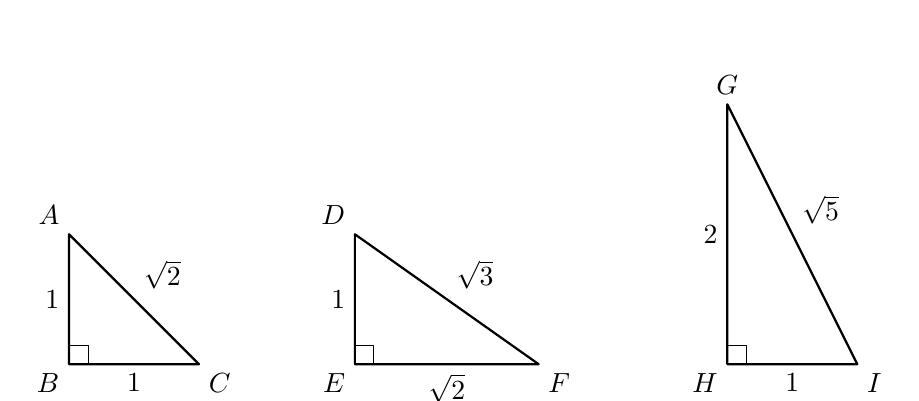
\begin{tikzpicture}[scale=1.1, line cap=round, line join=round]
    % Triangle 1: ABC
    \coordinate (B) at (0, 0);
    \coordinate (C) at (1.5, 0);
    \coordinate (A) at (0, 1.5);
    \draw[thick] (A) -- (B) -- (C) -- cycle;
    \draw (0, 0.22) -- (0.22, 0.22) -- (0.22, 0);
    \node[above left] at (A) {$A$};
    \node[below left] at (B) {$B$};
    \node[below right] at (C) {$C$};
    \node[left] at (0, 0.75) {$1$};
    \node[below] at (0.75, 0) {$1$};
    \node[above right] at (0.75, 0.75) {$\sqrt{2}$};

    % Triangle 2: DEF
    \begin{scope}[xshift=3.3cm]
    \coordinate (E) at (0, 0);
    \coordinate (F) at ({1.5*1.4142}, 0);
    \coordinate (D) at (0, 1.5);
    \draw[thick] (D) -- (E) -- (F) -- cycle;
    \draw (0, 0.22) -- (0.22, 0.22) -- (0.22, 0);
    \node[above left] at (D) {$D$};
    \node[below left] at (E) {$E$};
    \node[below right] at (F) {$F$};
    \node[left] at (0, 0.75) {$1$};
    \node[below] at ({0.75*1.4142}, 0) {$\sqrt{2}$};
    \node[above right] at ({0.75*1.4142}, 0.75) {$\sqrt{3}$};
    \end{scope}

    % Triangle 3: GHI
    \begin{scope}[xshift=7.6cm]
    \coordinate (H) at (0, 0);
    \coordinate (I) at (1.5, 0);
    \coordinate (G) at (0, 3.0);
    \draw[thick] (G) -- (H) -- (I) -- cycle;
    \draw (0, 0.22) -- (0.22, 0.22) -- (0.22, 0);
    \node[above] at (G) {$G$};
    \node[below left] at (H) {$H$};
    \node[below right] at (I) {$I$};
    \node[left] at (0, 1.5) {$2$};
    \node[below] at (0.75, 0) {$1$};
    \node[above right] at (0.75, 1.5) {$\sqrt{5}$};
    \end{scope}
\end{tikzpicture}
\end{center}

\begin{align*}
\overline{AC}^2 &= \overline{AB}^2 + \overline{BC}^2 = 1^2 + 1^2 = 2, \\
\overline{DF}^2 &= \overline{DE}^2 + \overline{EF}^2 = 1^2 + (\sqrt{2})^2 = 3, \\
\overline{GI}^2 &= \overline{GH}^2 + \overline{HI}^2 = 2^2 + 1^2 = 5.
\end{align*}
但是由第一冊第七章 § 2 中推論 2 可證 $x^2-2=0, x^2-3=0$ 及 $x^2-5=0$ 沒有「有理根」。所以 $\sqrt{2}, \sqrt{3}$ 及 $\sqrt{5}$ 都是不屬於有理數系的實數。因此，當我們在直線上取一點 $x$ 使得 $\overline{Ox}=\overline{AC}$（或 $\overline{DF}$ 或 $\overline{GI}$）就可以看出 $x$ 不是有理數點。

不屬於有理數系的實數有很多很多，上面三個數不過是隨便舉的幾個簡單的例子而已。

\subsubsection*{1-3 總結本節的討論，我們把有理數系與實數系間的關係扼要的敘述如下：}

\begin{enumerate}[(i)]
    \item 有理數系是實數系中一個到處稠密的子集。但是實數系除了有理數之外，還包含有許多許多不是有理數的數，通常（相對地）叫做無理數。（註\footnote{中文的「有理數」譯自「rational number」；「無理數」譯自「irrational number」。其實 rational 是 ratio 的形容詞，所以應該譯成「比數」和「非比數」才對。但是很不幸的當年翻譯者把上述「rational」及「irrational」誤譯成「有理」及「無理」。如今以訛傳訛，沿用至今。現在似乎不更正反而比更正它還「有理」些。特此註明。}）
    \item 因為有理數系在實數系中到處稠密，所以我們可以用有理數的「數列」去「逼近」任何一個給定實數。換句話說，任何一個給定實數都是某一適當的有理數數列的極限。
\end{enumerate}
我們將在下一節中，用實例詳細解釋第 (ii) 點。

\subsubsection*{習題 3-1}

\begin{enumerate}
    \item 寫出 $\sqrt{2+\sqrt{2}}$ 和 $\sqrt{2-\sqrt{2}}$ 都能滿足的整數係數多項式方程式。
    \item 分別寫出下列各數能滿足的整數係數多項式方程式：
    \begin{enumerate}[(i)]
        \item $\sqrt{2+\sqrt{3}}$。
        \item $\sqrt[3]{3+\sqrt{3}}$。
        \item $\sqrt[4]{3+\sqrt{3+\sqrt{2}}}$。
        \item $\sqrt{2+\sqrt{3+\sqrt{2}}}$。
    \end{enumerate}
    \item 利用圓規和直尺作出長度如下的各線段：
    \begin{enumerate}[(i)]
        \item $\sqrt{2+\sqrt{2}}$。
        \item $\sqrt{3+\sqrt{2+\sqrt{2}}}$。
        \item $\sqrt{5-\sqrt{3}}$。
        \item $\sqrt{\sqrt{6}-1}$。
    \end{enumerate}
    \item 證明在兩個不同的有理數 $a, b$ 之間，存在無限多有理數 $x$，使得 $a < x < y$\phantomsection\label{note:b2-ch3-ex3-1-q4-xy}.
    \item 請找出下列“證明”中的錯誤：$a \neq b$，令 $c = \frac{a+b}{2}$，\\
    所以 $2c = a+b$, $2c(a-b) = (a+b)(a-b) = a^2-b^2$,\\
    $\therefore b^2-2bc = a^2-2ac$。兩邊各加上 $c^2$ 得
    \[
    (b-c)^2 = b^2-2bc+c^2 = a^2-2ac+c^2 = (a-c)^2.
    \]
    所以 $b-c = a-c$，所以 $b=a$。
\end{enumerate}

\subsection{二分逼近法}\label{sec:b2_3-2}

在引言裡我們已經很具體地指出實數系是由度量所產生的數系，其中包含的數比有理數系包含的數要多得多。不能用有理數來表示的長度，是不是可以用有理數來表示它的近似值呢？這就是 § 1-3 提出的，也就是這一節所要詳細討論的。

\subsubsection*{2-1 事實上，以十進位 (decimal number system) 數字法寫成的有限位數小數已不敷表示所有的有理數。在第二章，§ 6 的例子中，我們已討論了如何以有限小數去逼近 $\frac{2}{3}$，就是十等分逼近法。當我們用 3 去除 2，即逐步得到下列諸式：}

\begin{align}
2 = 0.6 \times 3 + 0.2 &\implies 0.6 < \frac{2}{3} < 0.7, \tag{1}\label{eq:b2-ch3-div-1} \\
2 = 0.66 \times 3 + 0.02 &\implies 0.66 < \frac{2}{3} < 0.67, \tag{2}\label{eq:b2-ch3-div-2} \\
&\ \ \cdots\cdots\cdots\cdots\cdots\cdots\cdots\cdots \notag \\
2 = 0.\underbrace{66\dots 66}_{n} \times 3 + 0.\underbrace{00\dots 0}_{n-1}2 &\implies 0.\underbrace{66\dots 66}_{n} < \frac{2}{3} < 0.\underbrace{66\dots 67}_{n}. \tag{$n$}\label{eq:b2-ch3-div-n}
\end{align}

以上諸式可用直線坐標系加以圖解說明如下：

\begin{center}
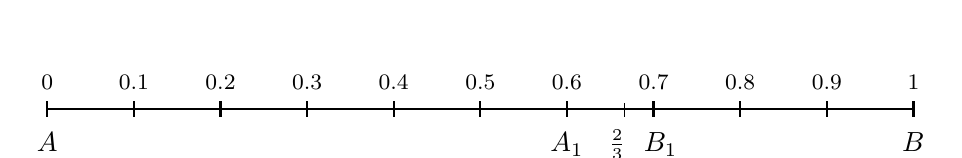
\begin{tikzpicture}[x=11.0cm, y=1cm]
    \draw[thick] (0, 0) -- (1, 0);
    \foreach \x in {0, 0.1, 0.2, 0.3, 0.4, 0.5, 0.6, 0.7, 0.8, 0.9, 1.0} {
        \draw[thick] (\x, 0.1) -- (\x, -0.1);
    }
    \node[above, font=\footnotesize] at (0, 0.12) {$0$};
    \node[above, font=\footnotesize] at (0.1, 0.12) {$0.1$};
    \node[above, font=\footnotesize] at (0.2, 0.12) {$0.2$};
    \node[above, font=\footnotesize] at (0.3, 0.12) {$0.3$};
    \node[above, font=\footnotesize] at (0.4, 0.12) {$0.4$};
    \node[above, font=\footnotesize] at (0.5, 0.12) {$0.5$};
    \node[above, font=\footnotesize] at (0.6, 0.12) {$0.6$};
    \node[above, font=\footnotesize] at (0.7, 0.12) {$0.7$};
    \node[above, font=\footnotesize] at (0.8, 0.12) {$0.8$};
    \node[above, font=\footnotesize] at (0.9, 0.12) {$0.9$};
    \node[above, font=\footnotesize] at (1.0, 0.12) {$1$};

    \node[below, font=\normalsize] at (0, -0.18) {$A$};
    \node[below, font=\normalsize] at (0.6, -0.18) {$A_1$};
    \draw[thin] (0.6667, 0.08) -- (0.6667, -0.10);
    \node[below, font=\small] at (0.658, -0.14) {$\frac{2}{3}$};
    \node[below, font=\normalsize] at (0.708, -0.18) {$B_1$};
    \node[below, font=\normalsize] at (1.0, -0.18) {$B$};
\end{tikzpicture}
\end{center}

\eqref{eq:b2-ch3-div-1} 式在上述坐標系中的意義是：\\
當我們把線段 $\overline{AB}=[0, 1]$ 等分為 10 段，$\frac{2}{3}$ 位於其第七段 $\overline{A_1 B_1} = [0.6, 0.7]$ 中。

\eqref{eq:b2-ch3-div-2} 式在上述坐標系中的意義是：\\
當我們把線段 $\overline{A_1 B_1}=[0.6, 0.7]$ 再等分為 10 段後，$\frac{2}{3}$ 位於線段 $\overline{A_2 B_2} = [0.66, 0.67]$ 中。

以此類推，\eqref{eq:b2-ch3-div-n} 式的意義是：\\
當我們把線段 $\overline{A_{n-1} B_{n-1}} = [0.\underbrace{66\dots\dots 66}_{n-1}, 0.\underbrace{66\dots\dots 67}_{n-1}]$ 再等分為 10 段時，$\frac{2}{3}$ 位於線段 $\overline{A_n B_n} = [0.\underbrace{66\dots\dots 66}_{n}, 0.\underbrace{66\dots\dots 67}_{n}]$ 中。

依樣畫葫蘆，對任意實數 $\xi$ 我們亦可以用「有限小數」去逼近它。假設 $\xi$ 位於線段 $\overline{A_0 B_0}=[k, k+1]$ 內，（亦即 $(k < \xi < k+1)$。）逼近方法是：將線段 $\overline{A_0 B_0}$ 逐次用十等分法求出線段 $\overline{A_1 B_1}, \overline{A_2 B_2}, \dots\dots, \overline{A_n B_n}, \dots\dots$ 滿足下列性質：
\begin{enumerate}[(i)]
    \item $\overline{A_0 B_0} \supseteq \overline{A_1 B_1} \supseteq \overline{A_2 B_2} \supseteq \dots\dots \supseteq \overline{A_n B_n} \supseteq \dots\dots \supseteq \{\xi\}$。
    \item $\overline{A_n B_n} = \frac{1}{10^n} = \frac{1}{10}\overline{A_{n-1} B_{n-1}}$.（線段長）
    \item 如果以 $a_n, b_n$ 表示 $A_n, B_n$ 的坐標，顯然 $a_n, b_n$ 是 $n$ 位小數，而且 $b_n - a_n = \overline{A_n B_n} = \frac{1}{10^n}$。
    \[
    k = a_0 \le a_1 \le a_2 \le \cdots \le a_n \le \cdots \le \xi \le \cdots \le b_n \le \cdots \le b_2 \le b_1 \le b_0 = k+1.
    \]
    \item 所以 $\langle a_n \rangle$ 是一個遞增數列，極限為 $\xi$；$\langle b_n \rangle$ 是一個遞減數列，其極限為 $\xi$。
\end{enumerate}

\subsubsection*{2-2 二（等）分逼近法}

將上述「十等分逼近法」略加簡化，就得到本節要向大家介紹的「二等分逼近法」，簡稱為「二分逼近法」，或「二分法」。現在說明如下：

設某數 $\xi$ 位於線段 $\overline{A_0 B_0}=[a_0, b_0]$ 內（亦即 $a_0 < \xi < b_0$）。

\begin{center}
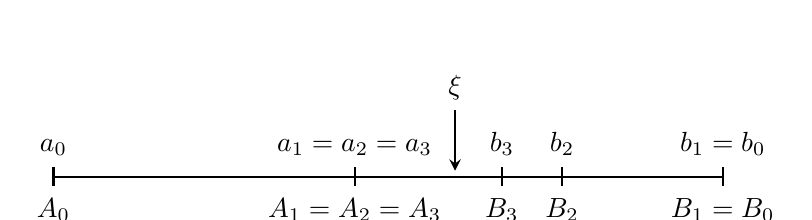
\begin{tikzpicture}[x=8.5cm, y=1cm]
    \draw[thick] (0,0) -- (1,0);
    
    % a0 / A0
    \draw[thick] (0, 0.12) -- (0, -0.12);
    \node[above] at (0, 0.15) {$a_0$};
    \node[below] at (0, -0.15) {$A_0$};

    % a1 = a2 = a3 / A1 = A2 = A3
    \draw[thick] (0.45, 0.12) -- (0.45, -0.12);
    \node[above] at (0.45, 0.15) {$a_1 = a_2 = a_3$};
    \node[below] at (0.45, -0.15) {$A_1 = A_2 = A_3$};

    % xi with arrow pointing down
    \draw[->, >=stealth, thick] (0.6, 0.85) -- (0.6, 0.08);
    \node[above] at (0.6, 0.85) {$\xi$};

    % b3 / B3
    \draw[thick] (0.67, 0.12) -- (0.67, -0.12);
    \node[above] at (0.67, 0.15) {$b_3$};
    \node[below] at (0.67, -0.15) {$B_3$};

    % b2 / B2
    \draw[thick] (0.76, 0.12) -- (0.76, -0.12);
    \node[above] at (0.76, 0.15) {$b_2$};
    \node[below] at (0.76, -0.15) {$B_2$};

    % b1 = b0 / B1 = B0
    \draw[thick] (1, 0.12) -- (1, -0.12);
    \node[above] at (1, 0.15) {$b_1 = b_0$};
    \node[below] at (1, -0.15) {$B_1 = B_0$};
\end{tikzpicture}
\end{center}

\begin{enumerate}[(i)]
    \item 我們將 $\overline{A_0 B_0}=[a_0, b_0]$ 等分為兩段，亦即 $[a_0, \frac{a_0+b_0}{2}]$ 和 $[\frac{a_0+b_0}{2}, b_0]$；而把 $\xi$ 所在的那一段叫做 $\overline{A_1 B_1}=[a_1, b_1]$（如果 $\xi = \frac{a_0+b_0}{2}$，就隨便取其中一段叫做 $\overline{A_1 B_1}=[a_1, b_1]$）。換句話說，當 $a_0 \le \xi \le \frac{a_0+b_0}{2}$ 時，$a_1 = a_0,\; b_1 = \frac{a_0+b_0}{2}$。當 $\frac{a_0+b_0}{2} \le \xi \le b_0$ 時，$a_1 = \frac{a_0+b_0}{2},\; b_1 = b_0$。這樣逐次用二等分由 $\overline{A_1 B_1}$ 求得 $\overline{A_2 B_2}, \dots\dots$，由 $\overline{A_{n-1} B_{n-1}}$ 求得 $\overline{A_n B_n}$。
    \item 如此逐步用二分法縮小範圍，就得到
    \begin{align*}
    \overline{A_0 B_0} = [a_0, b_0] &\supseteq \overline{A_1 B_1} = [a_1, b_1] \supseteq \dots\dots \supseteq \overline{A_n B_n} \\
    &= [a_n, b_n] \supseteq \overline{A_{n+1} B_{n+1}} \\
    &= [a_{n+1}, b_{n+1}] \supseteq \dots\dots \supseteq \{\xi\}.
    \end{align*}
    而且
    \[
    \overline{A_n B_n} = \frac{1}{2}\overline{A_{n-1} B_{n-1}} = \frac{1}{4}\overline{A_{n-2} B_{n-2}} = \dots\dots = \frac{1}{2^n}\overline{A_0 B_0} = \frac{1}{2^n}(b_0 - a_0).
    \]
    也就是
    \[
    a_0 \le a_1 \le a_2 \le \cdots \le a_n \le \cdots \le \xi \le \cdots \le b_n \le \cdots \le b_2 \le b_1 \le b_0.
    \]
    而且 $b_n - a_n = \frac{1}{2}(b_{n-1}-a_{n-1}) = \dots\dots = \frac{1}{2^n}(b_0-a_0)$ 當 $n$ 趨於無窮時其極限為 0，故有
    \item[(iii)] $\langle a_n \rangle$ 是一個遞增數列，$\langle b_n \rangle$ 是一個遞減數列，皆以 $\xi$ 為極限，也就是
    \[
    \lim_{n\to\infty} a_n = \xi = \lim_{n\to\infty} b_n.
    \]
    （$\langle a_n \rangle, \langle b_n \rangle$ 分別自 $\xi$ 的「左方」及「右方」逼近 $\xi$。）
    \item[(iv)] 如果 $a_0, b_0$ 都是有理數的話，顯然 $a_n, b_n$ 也都是有理數。所以這時 $\langle a_n \rangle, \langle b_n \rangle$ 都是有理數數列。而 (iii) 式就相當於我們最初所要說明的“任何一實數都是某一適當有理數數列的極限”.
\end{enumerate}

\subsubsection*{2-3 $\sqrt{2}$ 的近似值：}

現在以 $\xi = \sqrt{2},\; a_0 = 1,\; b_0 = 2$ 為例，說明如何去求 $\sqrt{2}$ 的近似值。

\begin{center}
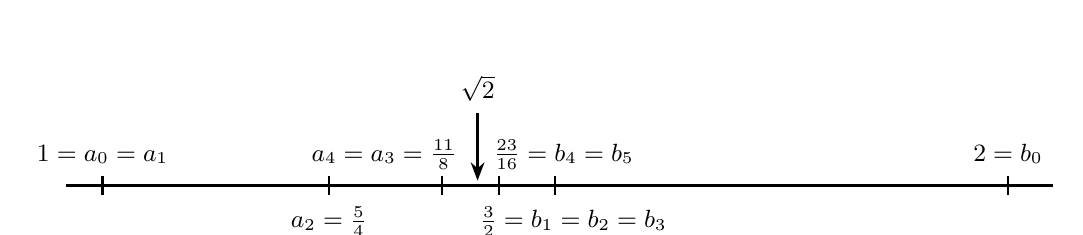
\begin{tikzpicture}[x=11.5cm, y=1cm, >=Stealth]
    \draw[thick] (-0.04, 0) -- (1.05, 0);
    
    % 1 = a0 = a1
    \draw[thick] (0, 0.12) -- (0, -0.12);
    \node[above, font=\small] at (0, 0.15) {$1 = a_0 = a_1$};

    % a2 = 5/4 = 0.25
    \draw[thick] (0.25, 0.12) -- (0.25, -0.12);
    \node[below, font=\small] at (0.25, -0.15) {$a_2 = \frac{5}{4}$};

    % a4 = a3 = 11/8 = 0.375 (anchored south-east so 11/8 sits above 0.375 and text extends left)
    \draw[thick] (0.375, 0.12) -- (0.375, -0.12);
    \node[anchor=south east, font=\small, inner sep=1pt] at (0.395, 0.16) {$a_4 = a_3 = \frac{11}{8}$};

    % sqrt(2) arrow at 0.4142 (passing cleanly between 11/8 and 23/16)
    \draw[->, thick] (0.4142, 0.92) -- (0.4142, 0.06);
    \node[above, font=\small] at (0.4142, 0.94) {$\sqrt{2}$};

    % 23/16 = b4 = b5 = 0.4375 (anchored south-west so 23/16 sits above 0.4375 and text extends right)
    \draw[thick] (0.4375, 0.12) -- (0.4375, -0.12);
    \node[anchor=south west, font=\small, inner sep=1pt] at (0.428, 0.16) {$\frac{23}{16} = b_4 = b_5$};

    % 3/2 = b1 = b2 = b3 = 0.5
    \draw[thick] (0.5, 0.12) -- (0.5, -0.12);
    \node[below, font=\small] at (0.52, -0.15) {$\frac{3}{2} = b_1 = b_2 = b_3$};

    % 2 = b0
    \draw[thick] (1, 0.12) -- (1, -0.12);
    \node[above, font=\small] at (1, 0.15) {$2 = b_0$};
\end{tikzpicture}
\end{center}

\begin{align}
\frac{1}{2}(a_0+b_0) = \frac{3}{2},&\quad \left(\frac{3}{2}\right)^2 = \frac{9}{4} > 2 \implies \frac{3}{2} > \sqrt{2}, \notag \\
\text{故}\quad a_1 = a_0 = 1,&\quad b_1 = \frac{3}{2}; \tag{1} \\
\frac{1}{2}(a_1+b_1) = \frac{5}{4},&\quad \left(\frac{5}{4}\right)^2 = \frac{25}{16} < 2 \implies \frac{5}{4} < \sqrt{2}, \notag \\
\text{故}\quad a_2 = \frac{5}{4},&\quad b_2 = b_1 = \frac{3}{2}; \tag{2} \\
\frac{1}{2}(a_2+b_2) = \frac{11}{8},&\quad \left(\frac{11}{8}\right)^2 = \frac{121}{64} < 2 \implies \frac{11}{8} < \sqrt{2}, \notag \\
\text{故}\quad a_3 = \frac{11}{8},&\quad b_3 = b_2 = \frac{3}{2}; \tag{3} \\
\frac{1}{2}(a_3+b_3) = \frac{23}{16},&\quad \left(\frac{23}{16}\right)^2 = \frac{529}{256} > 2 \implies \frac{23}{16} > \sqrt{2}, \notag \\
\text{故}\quad a_4 = a_3 = \frac{11}{8},&\quad b_4 = \frac{23}{16}; \tag{4} \\
\frac{1}{2}(a_4+b_4) = \frac{45}{32},&\quad \left(\frac{45}{32}\right)^2 = \frac{2025}{1024} < 2 \implies \frac{45}{32} < \sqrt{2}, \notag \\
\text{故}\quad a_5 = \frac{45}{32},&\quad b_5 = b_4 = \frac{23}{16}; \tag{5} \\
&\ \ \dots\dots\dots\dots\dots\dots\dots\dots \notag
\end{align}
如此逐步計算，每次只要檢驗「$\frac{1}{2}(a_{n-1}+b_{n-1})$ 的平方」和 2 之間的大小次序關係，就能確定 $\frac{1}{2}(a_{n-1}+b_{n-1})$ 應該是 $a_n$ 還是 $b_n$。顯然的，這樣所求得的 $a_n, b_n$ 和 $\sqrt{2}$ 有下列關係：
\[
a_n < \sqrt{2} < b_n,\quad b_n - a_n = \frac{1}{2^n}.
\]
我們可以把 $a_n$ 叫做 $\sqrt{2}$ 的一個「$n$ 階左近似值」，$b_n$ 叫做 $\sqrt{2}$ 的一個「$n$ 階右近似值」；它們和 $\sqrt{2}$ 的差小於 $\frac{1}{2^n}$。

\subsubsection*{習題 3-2}

\begin{enumerate}
    \item 用二分逼近法求方程式 $x^3+x-3=0$ 在 1 與 2 之間的根的左右近似值，準確到 $1/2^5$。
    \item 利用下列不等式，寫出 $\sqrt{3}+\sqrt{2}, \sqrt{3}-\sqrt{2}, \sqrt{3}\cdot\sqrt{2}$ 的逼近數列的前四項：
    \begin{alignat*}{2}
    1.4 &< \sqrt{2} < 1.5, &\qquad 1.7 &< \sqrt{3} < 1.8, \\
    1.41 &< \sqrt{2} < 1.42, &\qquad 1.73 &< \sqrt{3} < 1.74, \\
    1.414 &< \sqrt{2} < 1.415, &\qquad 1.732 &< \sqrt{3} < 1.733, \\
    1.4142 &< \sqrt{2} < 1.4143, &\qquad 1.7320 &< \sqrt{3} < 1.7321.
    \end{alignat*}
    \item 用二分逼近法求下列數的左右近似值，準確到 $1/2^5$。
    \begin{enumerate}[(a)]
        \item $\sqrt[3]{2}$。
        \item $\sqrt{5}$。
        \item $\sqrt{7}$。
        \item $\sqrt{\frac{3}{5}}$。
    \end{enumerate}
\end{enumerate}

\subsection{實數系的完備性與實數系的基本性質}\label{sec:b2_3-3}

\subsubsection*{3-1 對於加乘及不等式運算，實數系和有理數系具有完全相同的性質；為便於同學們參考與引用，將它們列述如下：}

對於實數系中的任意元素 $a, b, c \in \mathbb{R}$，恆有
\begin{enumerate}
    \item[(I)] $(a+b)+c = a+(b+c)$; $(ab)c = a(bc)$。\hfill 〔結合律〕
    \item[(II)] $a+b = b+a$; $ab = ba$。\hfill 〔交換律〕
    \item[(III)] $a+0 = 0+a = a$; $a\cdot 0 = 0\cdot a = 0$。\hfill 〔零的特性〕
    \item[(IV)] $a\cdot 1 = 1\cdot a = a$。\hfill 〔1 的特性〕
    \item[(V)] 對於任意 $a$，存在有唯一的一 $-a$，使得 $a+(-a) = 0$；\\
    對於任意 $a\neq 0$，存在有唯一的一 $\frac{1}{a}$，使得
    \[
    a\cdot \frac{1}{a} = 1. \hfill \text{〔可逆性〕}
    \]
    \item[(VI)] $a(b+c) = ab+ac$。\hfill 〔分配律〕
    \item[(I$'$)] $a>b \iff b<a$。
    \item[(II$'$)] $a>b \text{ 和 } b>c \implies a>c$。
    \item[(III$'$)] 對於任意實數 $a, b$，下列關係中有一種且僅有一種成立：
    \[
    a>b,\quad a=b \quad \text{或 } a<b.
    \]
    \item[(IV$'$)] $a>b \implies a+c < b+c$。\phantomsection\label{note:b2-ch3-prop-iv-prime}
    \item[(V$'$)] $a>b \text{ 和 } c>d \implies a+c > b+d$。
    \item[(VI$'$)] $a>b \text{ 和 } c>0 \implies ac>bc$。
    \item[(VII$'$)] $a>b \text{ 和 } c<0 \implies ac<bc$。
    \item[(VIII$'$)] 對於任意兩個正實數 $a, b>0$，恆存在有一夠大的正整數 $n$，使得 $na>b$.（通稱之為阿基米德性質。）
\end{enumerate}

\paragraph{註：} 當年阿基米德提出這個實數的基本性質，想必是從龜兔賽跑這個耐人尋味的故事中領悟而來的。玆有下圖為證：

\begin{center}
\begin{tikzpicture}[x=1cm, y=1cm, line cap=round, line join=round, >=Stealth]
    % Top segment: turtle stride length a
    \draw[|-|, thick] (2.0, 5.45) -- (3.0, 5.45);
    \node[above] at (2.5, 5.45) {$a$};
    \node[right, font=\normalsize] at (3.1, 5.45) {：龜步步幅};

    % Speech bubble for tortoise (auto-fitted box + pointer tail)
    \node[draw, thick, fill=white, rounded corners=6pt, align=center, font=\footnotesize, inner sep=6pt] (bubble) at (7.3, 3.85) {
        一萬、一萬零一$\cdots$\\
        阿基米德性質\\
        證起來真是\\
        累死我了！
    };
    \fill[white] ([xshift=-0.55cm, yshift=0.5pt]bubble.south) -- (6.2, 2.15) -- ([xshift=-0.20cm, yshift=0.5pt]bubble.south) -- cycle;
    \draw[thick] ([xshift=-0.55cm]bubble.south) -- (6.2, 2.15) -- ([xshift=-0.20cm]bubble.south);

    % Start indicator
    \draw[->, very thick] (0.5, 2.5) -- (0.5, 1.4);
    \node[draw, thick, fill=white, font=\footnotesize, inner sep=2pt] at (0.5, 2.2) {起點};

    % Upper line (Tortoise track)
    \draw[very thick, ->] (-0.5, 1.3) -- (10.2, 1.3);
    \draw[thick] (0.5, 1.45) -- (0.5, 1.15);
    \node[below, font=\normalsize] at (0.5, 1.15) {$0$};
    
    % Ticks along the track
    \draw[thick, dashed] (1.8, 1.45) -- (2.6, 1.45);
    \draw[thick] (3.6, 1.45) -- (3.6, 1.15);
    \draw[thick] (4.6, 1.45) -- (4.6, 1.15);
    \draw[thick] (5.6, 1.45) -- (5.6, 1.15);
    \draw[thick] (6.6, 1.45) -- (6.6, 1.15);

    % Tortoise on upper line at around x=5.6
    \begin{scope}[shift={(5.6, 1.45)}, scale=0.6]
        % Shell
        \draw[thick, fill=gray!15] (-0.9, 0) arc (180:0:0.9cm and 0.55cm) -- cycle;
        % Scutes pattern
        \draw[thin] (-0.5, 0.45) -- (-0.2, 0);
        \draw[thin] (0.5, 0.45) -- (0.2, 0);
        \draw[thin] (0, 0.55) -- (0, 0);
        \draw[thin] (-0.7, 0.25) -- (0.7, 0.25);
        % Head & neck
        \draw[thick] (0.8, 0.1) arc (-60:70:0.35cm and 0.25cm) -- (1.1, 0.4) arc (70:-120:0.2cm) -- (0.85, 0.05);
        \fill (1.15, 0.38) circle (1pt);
        % Legs
        \draw[thick] (-0.7, 0) -- (-0.8, -0.2) -- (-0.6, -0.2);
        \draw[thick] (-0.3, 0) -- (-0.4, -0.2) -- (-0.2, -0.2);
        \draw[thick] (0.4, 0) -- (0.3, -0.2) -- (0.5, -0.2);
        \draw[thick] (0.7, 0) -- (0.8, -0.2) -- (1.0, -0.2);
        % Tail
        \draw[thick] (-0.9, 0.05) -- (-1.1, 0.0);
    \end{scope}

    % Lower line (Hare track)
    \draw[very thick, ->] (-0.5, 0) -- (10.2, 0);
    \draw[thick] (0.5, 0.15) -- (0.5, -0.15);
    \node[above, font=\normalsize] at (0.5, 0.15) {$0$};

    % Tick at b
    \draw[thick] (8.3, 0.15) -- (8.3, -0.15);
    \node[below, font=\normalsize] at (8.3, -0.15) {$b$};

    % Sleeping Hare at position b
    \begin{scope}[shift={(8.3, 0.25)}, scale=0.65]
        % Body
        \draw[thick, fill=white] (-0.8, 0) arc (180:20:0.8cm and 0.5cm) arc (20:-160:0.8cm and 0.3cm) -- cycle;
        % Head
        \draw[thick, fill=white] (-0.6, 0.2) circle (0.3cm);
        % Closed eye
        \draw[thick] (-0.7, 0.2) arc (180:360:0.1cm and 0.05cm);
        % Ears lying back
        \draw[thick] (-0.4, 0.4) .. controls (0.2, 0.8) .. (0.7, 0.5) .. controls (0.2, 0.4) .. (-0.3, 0.3);
        \draw[thick] (-0.5, 0.45) .. controls (0.1, 0.95) .. (0.8, 0.7) .. controls (0.3, 0.55) .. (-0.4, 0.35);
        % Paws & Tail
        \draw[thick] (0.7, 0.1) arc (-30:150:0.2cm and 0.15cm);
        \draw[thick] (-0.2, -0.15) arc (0:180:0.2cm and 0.1cm);
    \end{scope}

    % Snoring Zzz
    \node[font=\footnotesize] at (7.6, 0.55) {$z$};
    \node[font=\small] at (7.4, 0.8) {$z$};
    \node[font=\normalsize] at (7.6, 1.05) {$Z$};
\end{tikzpicture}
\end{center}

\subsubsection*{3-2 實數系的完備性：}

由上節所述，我們看出實數系與有理數系在加、乘及不等式的運算有完全相同的性質。但是實數系與有理數系在極限方面卻有很重大的差異。譬如在上一節中我們所求得的兩個有理數數列 $\langle a_n \rangle, \langle b_n \rangle$。
\begin{gather*}
1 = a_0 \le a_1 \le a_2 \le \cdots \le a_n \le \cdots \le \sqrt{2} \le \cdots \le b_n \le \cdots \le b_2 \le b_1 \le b_0 = 2, \\
\lim_{n\to\infty}(b_n-a_n) = \lim_{n\to\infty}\frac{1}{2^n} = 0.
\end{gather*}
它們的極限 $\sqrt{2}$ 卻不是有理數，也就是說
\[
a_n, b_n \in \mathbb{Q};\quad \text{但是 } \lim_{n\to\infty} a_n = \sqrt{2} = \lim_{n\to\infty} b_n \notin \mathbb{Q}.
\]
換句話說，一個完全由有理數所組成的數列，它的極限不一定是有理數。所以對於極限來說，有理數系顯然不夠完備。但是相反的實數系對於極限來說是完備的。實數系的完備性可以敘述成好幾種不同的形式。我們在這裡先敘述下面兩種形式：

(IX$'$) 完備性（第一形式）：設 $\langle a_n \rangle, \langle b_n \rangle$ 是兩個實數數列滿足下列性質：
\begin{enumerate}[(i)]
    \item $a_1 \le a_2 \le \dots\dots \le a_n \le \dots\dots \le b_n \le \dots\dots \le b_2 \le b_1$,
    \item $\lim_{n\to\infty}(b_n-a_n) = 0$。
\end{enumerate}
就必定存在有一個實數 $\xi$，使得
\[
\lim_{n\to\infty} a_n = \xi = \lim_{n\to\infty} b_n.
\]
完備性（第二形式）：如果 $\langle a_n \rangle$ 是一個有上界 $c$ 的遞增數列，$a_1 \le a_2 \le \dots\dots \le c$。就會有一個實數 $\xi$，使得
\[
\lim_{n\to\infty} a_n = \xi \le c.
\]
上述完備性 (IX$'$) 和前述性質 (I)$\sim$(VI), (I$'$$\sim$(VIII$'$) 就構成實數系的一組基本性質。所有其他的實數系性質都是它們的邏輯推論。

我們在這裡再強調一次；實數系與有理數系間最基本的差異，便在於上述的完備性。事實上，實數系的完備性乃是微積分學的基礎。由於同學們目前所知有限，在現階段無法對此深切體會。不過我們將以下列定理為例，來說明完備性的一個應用。

\subsubsection*{習題 3-3}

\begin{enumerate}
    \item 證明任意兩實數 $a, b$ 之間，一定存在有理數 $c$，使得 $a < c < b$（用阿基米德性質）
    \item 利用實數的完備性，證明下列敘述：\\
    設 $\langle a_n \rangle$ 是一個遞減數列，並且有一個下界 $c$，（即 $c < a_n\; \forall n$），則數列 $\langle a_n \rangle$ 的極限存在，而且 $c \le \lim_{n\to\infty} a_n$。
    \item 如果 $a>0$，證明數列 $a_1 = a, a_2 = 2a, \dots\dots a_n = na \dots\dots$ 沒有上限。由此證明阿基米德性質：$a>0, b$ 任意實數，則存在正整數 $n$，使得 $nc > d$\phantomsection\label{note:b2-ch3-ex3-3-q3-nc-d}.
    \item 設 $a, b$ 是兩個正實數，證明：
    \begin{enumerate}[(i)]
        \item 如果 $a>b$，則 $\lim_{n\to\infty}\left(\frac{a}{b}\right)^n = \infty$。
        \item 如果 $a<b$，則 $\lim_{n\to\infty}\left(\frac{a}{b}\right)^n = 0$。
    \end{enumerate}
    \item 設 $a, b$ 是兩個正實數，而且 $a>1$，利用阿基米德性質，證明存在自然數 $n$，使 $a^n > b$ 成立。
    \item 設 $n$ 是自然數，$a$ 是實數，證明
    \[
    (1+a)^n \ge 1+na.
    \]
    \item 如果 $P$ 是質數，$P>0$，證明 $\sqrt{P}$ 是無理數。
    \item 設 $\alpha, \beta, \gamma$ 是三個正實數，
    \begin{enumerate}[(i)]
        \item 如果 $\alpha < \beta$，證明 $\frac{\alpha}{1+\alpha} < \frac{\beta}{1+\beta}$。
        \item 如果 $\alpha+\beta = \gamma$，證明 $\frac{\gamma}{1+\gamma} < \frac{\alpha}{1+\alpha} + \frac{\beta}{1+\beta}$。
    \end{enumerate}
\end{enumerate}

\subsection{中間值定理}\label{sec:b2_3-4}

下述定理是實數系完備性的一個重要推論。

\begin{theorem}[多項式函數的中間值定理]
設 $f(x)$ 是一個實係數多項式，而 $a, b$ 為兩個給定實數，且 $a < b$。如果 $f(a)$ 和 $f(b)$ 異號，那麼在 $a, b$ 之間一定至少有一個 $f(x)=0$ 的根。（至少有一個實數 $\xi, a < \xi < b$ 而且 $f(\xi)=0$。）
\end{theorem}

如果我們畫一個圖

\begin{center}
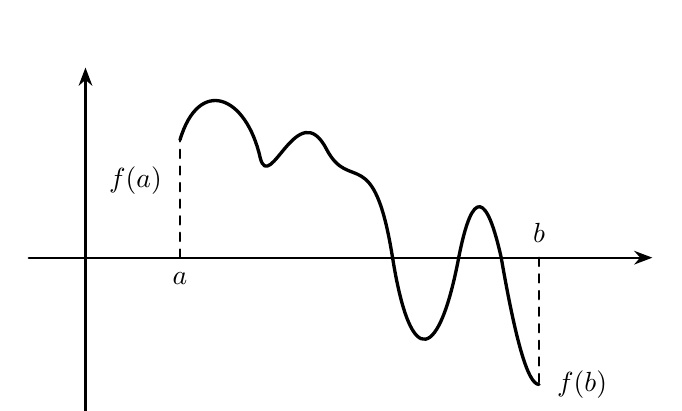
\begin{tikzpicture}[x=1.2cm, y=1.15cm, line cap=round, line join=round, >=Stealth]
    % Axes
    \draw[thick, ->] (-0.6, 0) -- (6.0, 0);
    \draw[thick, ->] (0, -1.8) -- (0, 2.1);

    % Curve starting at (a, f(a)) and ending cleanly at (b, f(b)), crossing x-axis 3 times
    \coordinate (A) at (1.0, 1.3);
    \coordinate (B) at (4.8, -1.4);

    \draw[very thick] (1.0, 1.3) .. controls (1.2, 2.0) and (1.7, 1.8) .. (1.85, 1.1)
                                .. controls (1.95, 0.7) and (2.25, 1.8) .. (2.55, 1.2)
                                .. controls (2.8, 0.7) and (3.05, 1.3) .. (3.25, 0)
                                .. controls (3.45, -1.3) and (3.75, -1.1) .. (3.95, 0)
                                .. controls (4.1, 0.8) and (4.25, 0.7) .. (4.4, 0)
                                .. controls (4.55, -0.9) and (4.68, -1.4) .. (4.8, -1.4);

    % Dashed vertical lines at a and b
    \draw[dashed, thick] (1.0, 0) -- (A);
    \draw[dashed, thick] (4.8, 0) -- (B);

    % Points and labels
    \node[below=2pt, font=\normalsize] at (1.0, 0) {$a$};
    \node[left=3pt, font=\normalsize] at (1.0, 0.85) {$f(a)$};
    \node[above=2pt, font=\normalsize] at (4.8, 0) {$b$};
    \node[right=3pt, font=\normalsize] at (B) {$f(b)$};
\end{tikzpicture}
\end{center}

那麼定理 1，在直觀上是顯而易見的。
\paragraph{【證明】}
顯然我們只需要討論 $f(a)>0, f(b)<0$ 的情形，因為對於 $f(a)<0, f(b)>0$ 的情形，我們只要改為討論 $-f(x)$ 就可以了。現在取 $a_0 = a, b_0 = b$，利用 § 2 中的二分法討論如下：
\[
\begin{cases}
\text{如果 } f\left(\frac{a_0+b_0}{2}\right) = 0, & \text{則定理 1 已經成立了，不必再多作討論。} \\[1em]
\text{如果 } f\left(\frac{a_0+b_0}{2}\right) > 0, & \text{就取 } a_1 = \frac{a_0+b_0}{2},\; b_1 = b_0. \\[1em]
\text{如果 } f\left(\frac{a_0+b_0}{2}\right) < 0, & \text{就取 } a_1 = a_0,\; b_1 = \frac{a_0+b_0}{2}.
\end{cases}
\]

\begin{center}
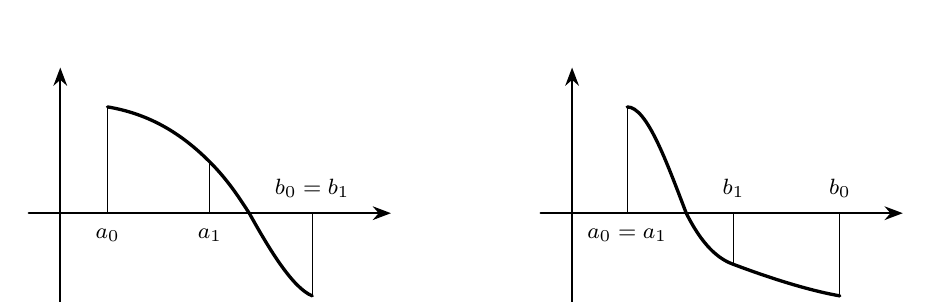
\begin{tikzpicture}[scale=1.0, line cap=round, line join=round, >=Stealth]
    % Diagram 1: f((a0+b0)/2) > 0
    \begin{scope}[xshift=0cm]
        \draw[thick, ->] (-0.4, 0) -- (4.2, 0);
        \draw[thick, ->] (0, -1.25) -- (0, 1.85);
        
        % Curve from a0 (0.6, 1.35) through a1 (1.9, 0.65) crossing at 2.4 to b0=b1 (3.2, -1.05)
        \draw[very thick] (0.6, 1.35) .. controls (1.2, 1.25) and (1.6, 0.95) .. (1.9, 0.65)
                                      .. controls (2.15, 0.4) and (2.3, 0.15) .. (2.4, 0)
                                      .. controls (2.65, -0.45) and (2.95, -0.95) .. (3.2, -1.05);

        % Vertical segments to curve (matching original scan p. 14)
        \draw[thin] (0.6, 0) -- (0.6, 1.35);
        \draw[thin] (1.9, 0) -- (1.9, 0.65);
        \draw[thin] (3.2, 0) -- (3.2, -1.05);

        \node[below=2pt, font=\footnotesize] at (0.6, 0) {$a_0$};
        \node[below=2pt, font=\footnotesize] at (1.9, 0) {$a_1$};
        \node[above=2pt, font=\footnotesize] at (3.2, 0) {$b_0 = b_1$};
    \end{scope}

    % Diagram 2: f((a0+b0)/2) < 0
    \begin{scope}[xshift=6.5cm]
        \draw[thick, ->] (-0.4, 0) -- (4.2, 0);
        \draw[thick, ->] (0, -1.25) -- (0, 1.85);
        
        % Curve from a0=a1 (0.7, 1.35) crossing at 1.45 through b1 (2.05, -0.65) to b0 (3.4, -1.05)
        \draw[very thick] (0.7, 1.35) .. controls (0.95, 1.35) and (1.2, 0.65) .. (1.45, 0)
                                      .. controls (1.65, -0.4) and (1.85, -0.58) .. (2.05, -0.65)
                                      .. controls (2.5, -0.82) and (3.0, -0.98) .. (3.4, -1.05);

        % Vertical segments to curve (matching original scan p. 14)
        \draw[thin] (0.7, 0) -- (0.7, 1.35);
        \draw[thin] (2.05, 0) -- (2.05, -0.65);
        \draw[thin] (3.4, 0) -- (3.4, -1.05);

        \node[below=2pt, font=\footnotesize] at (0.7, 0) {$a_0 = a_1$};
        \node[above=2pt, font=\footnotesize] at (2.05, 0) {$b_1$};
        \node[above=2pt, font=\footnotesize] at (3.4, 0) {$b_0$};
    \end{scope}
\end{tikzpicture}
\end{center}

總之，除了 $f\left(\frac{a_0+b_0}{2}\right) = 0$ 這個顯然成立的情形以外，我們可以用二分法從 $[a_0, b_0]$ 中選得半段 $[a_1, b_1]$ 依然保有 $f(a_1)>0, f(b_1)<0$ 這個原來的假設條件。所以我們又可以同樣地用二分法從 $[a_1, b_1]$ 求得 $[a_2, b_2]$，並且依然保有 $f(a_2)>0, f(b_2)<0$ 這個原始條件。

如此逐次二等分，假如在某一次的等分點 $\frac{a_n+b_n}{2}$ 滿足 $f\left(\frac{a_n+b_n}{2}\right) = 0$，則定理 1 就成立了，也不必再多作討論。假如對每一次的等分點 $\frac{a_n+b_n}{2}$，$f\left(\frac{a_n+b_n}{2}\right)$ 都不是 0，那麼可以按上述二分法繼續不斷的進行，就能得到滿足下列性質的數列 $\langle a_n \rangle$ 和 $\langle b_n \rangle$：
\begin{enumerate}[(i)]
    \item $f(a_n)>0, f(b_n)<0, n=1, 2, 3, \dots\dots$
    \item $a = a_0 \le a_1 \le a_2 \le \dots\dots \le a_n \le \dots\dots \le b_n \le \dots\dots \le b_2 \le b_1 \le b_0$。
    \item $\lim_{n\to\infty}(b_n-a_n) = \lim_{n\to\infty}\frac{b-a}{2^n} = 0$。
\end{enumerate}
由實數的完備性及 (ii), (iii) 得知存在一個實數 $\xi$，
\[
\lim_{n\to\infty} a_n = \xi = \lim_{n\to\infty} b_n
\]
又由 (i) 知道
\[
\lim_{n\to\infty} f(a_n) \ge 0 \quad \text{和} \quad \lim_{n\to\infty} (b_n) \le 0\phantomsection\label{note:b2-ch3-lim-bn}.
\]
因為 $f(x)$ 是多項式，由極限的四則運算可以得到：
\begin{align*}
\lim_{n\to\infty} f(a_n) &= f(\lim_{n\to\infty} a_n) = f(\xi) \ge 0, \\
\lim_{n\to\infty} f(b_n) &= f(\lim_{n\to\infty} b_n) = f(\xi) \le 0.
\end{align*}
因為 $f(\xi)\ge 0$ 和 $f(\xi)\le 0$ 需要同時成立，所以 $f(\xi)=0$。
\hfill（定理 1 證畢）

\paragraph{【例 1】} $f(x) = 2x^2+7x+1$ \\
因 $f(0) = 1 > 0$ 及 $f(-1) = -4 < 0$，\\
所以 $f(x)=0$ 在 $[-1, 0]$ 之間有一實根。\\
又因 $f(-3) = -2 < 0$ 及 $f(-4) = 5 > 0$，\\
所以 $f(x)=0$ 在 $[-4, -3]$ 之間也有一實根。

\begin{prop}[推論]
設 $a$ 是一個正實數，$n$ 是一個正整數，那麼就有一個唯一的正實數 $\xi$，使得 $\xi^n = a$.（我們因而用 $\sqrt[n]{a}$ 表示滿足 $x^n = a$ 的唯一正實數 $\xi$。）
\end{prop}
\paragraph{【證明】} 令 $f(x) = x^n - a,\; b = a+1$。顯然有
\begin{align*}
f(0) &= -a < 0, \\
f(b) &= (1+a)^n - a \ge 1+(n-1)a > 0,
\end{align*}
由定理 1 得知 $[0, b]$ 之間至少有 $f(x)=0$ 的一個實根。

現在我們再證唯一性；設 $\xi_1, \xi_2$ 是兩個滿足 $f(x)=0$ 的正實數：
\[
\xi_1^n - a = 0,\quad \xi_2^n - a = 0.
\]
兩式相減，得到
\[
\xi_1^n - \xi_2^n = 0,\quad \text{亦即 } \xi_1^n = \xi_2^n.
\]
所以 $\xi_1$ 必定和 $\xi_2$ 相同，要不然的話，由性質 (III$'$) 有
\[
\xi_1 > \xi_2,\quad \text{或 } \xi_1 < \xi_2.
\]
但是
\begin{align*}
\xi_1 > \xi_2 > 0 &\implies \xi_1^n > \xi_2^n > 0, \\
0 < \xi_1 < \xi_2 &\implies 0 < \xi_1^n < \xi_2^n.
\end{align*}
這顯然和 $\xi_1^n = \xi_2^n$ 相矛盾。換句話說，$\xi_1 \neq \xi_2$ 是不可能的，所以只好 $\xi_1 = \xi_2$。但是 $\xi_1, \xi_2$ 是 $f(x)=0$ 的任意正根，故 $f(x)=0$ 的正根只有一個。

定理 1 的另外一個重要推論可寫成：

\begin{theorem}
$f(x)$ 是一個奇數次實係數多項式，那麼方程式 $f(x)=0$ 至少有一實根。
\end{theorem}
\paragraph{【證明】} 基於定理 1，我們只要能求得兩個實數 $\alpha, \beta$，使得奇數次多項式 $f(x)$ 在 $\alpha, \beta$ 的值異號。（即 $f(\alpha)f(\beta)<0$ 就可以了。）當然我們還可以假設 $f(x)$ 的首項係數是正的，要不然我們只要把 $f(x)$ 換成 $-f(x)$ 來討論就行了。

設 $f(x) = a_n x^n + a_{n-1} x^{n-1} + \dots\dots + a_0,\; a_n > 0,\; n$ 為奇數，我們希望找到一個大的正數 $k$，使得
\[
a_n k^n > |a_{n-1} k^{n-1} + \dots\dots + a_0|.
\]
那麼，
\begin{align*}
f(k) &= a_n k^n + a_{n-1} k^{n-1} + \dots\dots + a_0 \\
&\ge a_n k^n - |a_{n-1} k^{n-1} + \dots\dots + a_0| \\
&\ge 0.
\end{align*}
另一方面，
\begin{align*}
f(-k) &= a_n (-k)^n + a_{n-1} (-k)^{n-1} + \dots\dots + a_0 \\
&= -[(a_n k^n) - (a_{n-1} (-k)^{n-1} + \dots\dots + a_0)] \\
&\le -(a_n k^n - |a_{n-1} k^{n-1} + \dots\dots + a_0|) \\
&< 0.
\end{align*}
那麼就可以運用定理 1 而得到一個實根了。

現在的問題就是如何找到這樣一個 $k$，我們知道對於任一實數 $k > 1$，且 $m = \operatorname{Max}(|a_{n-1}|, \dots\dots, |a_0|)$，則
\begin{align*}
|a_{n-1} k^{n-1} + \dots\dots + a_0| &\le |a_{n-1} k^{n-1}| + \dots\dots + |a_0| \\
&\le n m k^{n-1}
\end{align*}
比較 $a_n k^n$ 與 $n m k^{n-1}$，我們知道如果取一個正整數 $k$ 滿足 $k a_n > n m$，那麼 $a_n k^n > n m k^{n-1}$ 當然成立。也就是說 $a_n k^n > n m k^{n-1} \ge |a_{n-1} k^{n-1} + \dots\dots + a_0|$。總括以上解析可知，只要按照阿基米德性質取一個正整數 $k$，使得 $k a_n > n m$，就有
\begin{align*}
f(k) &> 0 \\
f(-k) &< 0
\end{align*}
這個定理也就得證了。

\paragraph{【例 2】}
\begin{enumerate}[(i)]
    \item $x^5+10x^2+3=0$ 至少有一個負實根。
    \item $x^7+6x^4-1=0$ 至少有一個正實根。
\end{enumerate}

\paragraph{注意：} 定理 2 中 $n$ 是奇數是一個不可缺少的條件，譬如 $x^2+1=0$ 就顯然沒有實根。因為對於任何實數 $a, a^2 \ge 0$，故有
\[
f(a) = a^2+1 \ge 1 \ge 0.
\]

\subsubsection*{習題 3-4}

\begin{enumerate}
    \item 找出下列各多項式方程式的所有實根的位置（在那兩個相鄰整數之間）：
    \begin{enumerate}[(i)]
        \item $x^4-10x^2+1=0$.（有四實根）
        \item $x^3-3x^2+3x-4=0$.（有一實根）
        \item $2x^5-5x^4-7x^3+16x^2+3x-3=0$.（有五實根）
    \end{enumerate}
    \item 設 $f(x)$ 是一個多項式，$a, b$ 是兩個實根\phantomsection\label{note:b2-ch3-ex3-4-q2-roots}，$a < b$。如果實數 $c$ 在 $f(a)$ 與 $f(b)$ 之間（例如 $f(a) < c < f(b)$），證明存在實數 $\xi, a < \xi < b$，使得 $f(\xi) = c$。
    \item 如果在實係數多項式 $f(x) = a_0 + a_1 x + \dots\dots + a_n x^n$ 中 $a_0$ 與 $a_n$ 異號（即 $a_0 a_n < 0$），證明 $f(x)=0$ 必有一正實根。
    \item 下列方程式各有一個正實數根，利用多項式函數的中間值定理，求它們的近似值至三位小數：
    \begin{enumerate}[(i)]
        \item $x^2-5=0$。
        \item $x^2-4x-3=0$。
        \item $x^3-4=0$。
        \item $x^3-9x-10=0$。
    \end{enumerate}
    \item 設函數 $y=f(x)=3x^3-1$，利用多項式函數的中間值定理，證明在 0 與 1 之間有一個實數 $a$，使 $f(a)=a$ 成立。
\end{enumerate}

\subsection{連續函數}\label{sec:b2_3-5}

在證明多項式的中間值定理時，我們用到了兩個主要條件，一個就是實數的完備性，還有一個就是多項式函數的連續性，所謂連續性就是對於任意數列 $\langle a_n \rangle, a_n \to \xi$，我們有
\begin{equation}\tag{1}
\lim_{n\to\infty} f(a_n) = f(\lim_{n\to\infty} a_n) = f(\xi)
\end{equation}
的關係。因此可以推問，對於一般滿足條件 (1) 的函數，中間值定理也成立嗎？為了討論這個問題，我們把這類函數叫做連續函數，本節就是要討論連續函數的中間值定理。

\begin{definition*}
設 $f: A \longrightarrow B$ 是一個函數，而 $\xi$ 是 $A$ 中的一點，如果對於 $A$ 中的任意數列 $\langle a_n \rangle, a_n \to \xi$，我們有 $\lim_{n\to\infty} f(a_n) = f(\xi)$ 的話，就說函數 $f$ 在 $\xi$ 點連續。如果 $f$ 在 $A$ 中每一點都連續，就說 $f$ 是 $A$ 上的一個連續函數，或簡稱為連續函數。
\end{definition*}

譬如多項式函數是連續函數。又如 $y = [x]$（$[\ ]$ 是高斯符號，表示小於或等於 $x$ 的最大整數，見第一冊第五章）是從實數到整數的一個函數，它在整數點不連續，在其他的點都連續。當然，不連續函數的例子還有很多，但在高中階段，我們用不著深究。

讓我們現在來考慮一個任意的連續函數 $f: A \longrightarrow B$，如果 $\xi$ 是 $A$ 中的一點，$\langle a_n \rangle, \langle b_n \rangle$ 是兩個趨近於 $\xi$ 的數列，而且
\[
b_1 \le b_2 \le \dots\dots \le b_n \le \dots\dots \le \xi \le \dots\dots \le a_n \le \dots\dots \le a_2 \le a_1.
\]
那麼由連續的定義，可以知道
\[
\lim_{n\to\infty} f(a_n) = \lim_{n\to\infty} f(b_n) = f(\xi).
\]
反過來我們還可以證明這也是連續函數的充分條件：\\
假設 $f: A \longrightarrow B$ 是一個函數，而 $\xi$ 是 $A$ 中的一點，如果對任意以 $\xi$ 為極限的遞減或遞增的數列 $\langle a_n \rangle$，都有 $\lim_{n\to\infty} f(a_n) = f(\xi)$，那麼函數 $f$ 在 $\xi$ 點連續。（因為證明複雜，在此略去不談）

\begin{theorem}[定理 $1'$（連續函數的中間值定理）]
設 $f(x)$ 是一個連續函數，而 $a, b$ 是兩個實數且 $a < b$。如果 $f(a)$ 和 $f(b)$ 異號，那麼在 $a, b$ 之間一定有一個 $f(x)=0$ 的根（即有一實數 $\xi, a < \xi < b$ 而且 $f(\xi)=0$）。
\end{theorem}
因為證明幾乎與定理 1 完全一樣，所以我們不在此贅述了。

\begin{prop}[推論]
設 $f(x)$ 是一個連續函數，$a, b$ 是兩個實數，而且 $a < b$，$f(a) \neq f(b)$。那麼對於任意一個介於 $f(a), f(b)$ 之間的數 $M$，一定有一個 $a, b$ 之間的實數 $\xi$，使得 $f(\xi)=M$。
\end{prop}
\paragraph{【證明】}
我們不妨假設 $f(a) < f(b)$.（因為 $f(a) > f(b)$ 時，可以同樣處理）。那麼 $M$ 滿足 $f(a) < M < f(b)$，如果考慮一個新的函數 $g$：
\[
g(x) = f(x) - M.
\]
那麼
\[
g(a) = f(a) - M < 0,\quad g(b) = f(b) - M > 0.
\]
因此根據定理 $1'$，一定有一實數 $\xi, a < \xi < b$，使得 $g(\xi)=0$。換句話說
\[
f(\xi)-M = 0 \quad \text{或} \quad f(\xi)=M.
\]

\subsubsection*{習題 3-5}

\begin{enumerate}
    \item 設函數 $y = f(x) = \frac{x^2+1}{2x-1}$，則 $f(0) = -1, f(1) = 2$ 符號相反，討論方程式 $f(x)=0$ 在 $0 \le x \le 1$ 中是否有解？
    \item 證明下列各函數是連續，並利用連續函數的中間值定理求根的位置（介於那兩個相接的整數之間）。
    \begin{enumerate}[(i)]
        \item $y = f(x) = x|x| - \frac{1}{2}$。
        \item $y = f(x) = |x+1| - |x - \frac{2}{3}|$。
    \end{enumerate}
    \item 下列函數各在那些點不連續？
    \begin{enumerate}[(i)]
        \item $y = f(x) = [x^2+1]$。
        \item $y = f(x) = |x|$。
        \item $y = f(x) = [\frac{x+1}{2}]x + 1$。
        \item $y = f(x) = x\cdot |x|$。
    \end{enumerate}
    \item 討論下列有理函數，各在那些點連續？
    \begin{enumerate}[(i)]
        \item $y = f(x) = \frac{x+2}{x^2-1}$。
        \item $y = f(x) = \frac{x-1}{x^2+1}$。
        \item $y = f(x) = \frac{1}{x} + \frac{1}{x+1} + \frac{1}{x-1}$。
    \end{enumerate}
    \item 證明 (i) $y = f(x) = \frac{1}{x}$，除了 $x = 0$ 以外連續。\\
    (ii) $y = f(x) = \frac{1}{ax+b},\; a\neq 0$，除了 $x = \frac{b}{a}$ 外連續\phantomsection\label{note:b2-ch3-ex3-5-q5-sign}.
    \item 證明多項式函數都是連續函數。
\end{enumerate}
 % 第三章 實數系及其基本性質
% =========================================================================
% 《高中數學實驗教材》第二冊（高一下） 
% 第四章 指數函數與對數函數
% =========================================================================

\section{指數函數與對數函數}\label{sec:b2_ch4}

對於每一個正實數 $a$，我們用 $a^n$ 表示 $n$ 個相乘的連乘積。例如：
\[
a^1 = a,\quad a^2 = a\cdot a,\quad a^3 = a\cdot a\cdot a,\quad \dots\dots\dots\dots,
\]
\[
a^{n+1} = a^n \cdot a,\quad \dots\dots \text{等}.
\]
所以指數符號 $a^n$ 只是 $a$ 自乘 $n$ 次的簡寫，而下列大家所熟悉的指數定則乃是乘法結合律的一個直接推論：
\begin{align}
a^n \cdot a^m &= a^{n+m} \label{eq:b2-ch4-intro-exp-rule-1} \\
(a^n)^m &= a^{nm} \label{eq:b2-ch4-intro-exp-rule-2}
\end{align}

在本章第一節中，我們將討論如何把指數的定義逐步推廣到負整數指數，分數指數及實數指數，使得推廣後的廣義指數符號 $a^\alpha\; (\alpha \in \mathbb{R})$ 依然滿足指數定則：
\begin{align}
a^\alpha \cdot a^\beta &= a^{\alpha+\beta} \label{eq:b2-ch4-intro-gen-rule-1} \\
(a^\alpha)^\beta &= a^{\alpha\beta} \label{eq:b2-ch4-intro-gen-rule-2}
\end{align}
當我們將指數的範圍推廣到全實數系後，$a^\alpha$ 中的 $\alpha$ 可以在實數系 $\mathbb{R}$ 中任意變更皆有明確的意義。所以 $y = a^x$ 是一個函數（參看第一冊第五章 § 3）。我們把它叫做指數函數。我們將在 § 2 中討論指數函數的重要特性，在 § 3 中討論指數函數的反函數——對數函數——及它的性質。指數函數與對數函數是研究許多自然現象及社會問題的重要工具。

\subsection{指數定則與指數定義的推廣}\label{sec:b2_4-1}

\subsubsection*{1-1 負整數指數的定義}

首先，我們要把指數的定義推廣到全整數系 $\mathbb{Z}$。

\begin{definition*}
對於正實數 $a$，我們定義 $a^0 = 1,\; a^{-n} = \frac{1}{a^n},\; n \in \mathbb{N}$。
\end{definition*}
\paragraph{【討論】} 假想我們所定義的 $a^0$ 和 $a^{-n}$ 依然滿足指數定則，那麼由下列計算可以看出 $a^0$ 必須等於 1，$a^{-n}$ 必須等於 $\frac{1}{a^n}$，這就是我們如此定義 $a^0$ 和 $a^{-n}$ 的原因：\\
因
\[
a^0 \cdot a^n = a^{0+n} = a^n, \quad \text{但是 } a^n \neq 0, \text{ 所以 } a^0 = 1.
\]
又
\[
a^{-n} \cdot a^n = a^{-n+n} = a^0 = 1, \quad \text{所以 } a^{-n} = \frac{1}{a^n}.
\]
同學們應該注意：上面所談的並不是 $a^0 = 1$ 的證明，因為在 $a^0$ 根本還沒有定義前，要去證明它等於什麼數是完全沒有意義的。同學們也許要問，$a^0$ 可不可以定義成其他的數呢？例如定義
\[
a^0 = 2,
\]
自然也沒有關係，但是這樣就破壞了指數定則，而我們的要點是：如何選擇適當的定義，使得指數定則仍然成立。要想辦到這一節，$a^0 = 2$ 就不行，而一定要 $a^0 = 1$ 才可以。這種選擇定義，使得某種良好性質得以保存，是在數學裏常用的手段。

反過來說，當我們採取定義 $a^0 = 1,\; a^{-n} = \frac{1}{a^n}$ 時，不難看出對所有 $h, k \in \mathbb{Z}$ 指數定則都成立：
\begin{align}
a^h \cdot a^k &= a^{h+k} \label{eq:b2-ch4-int-exp-1} \\
(a^h)^k &= a^{hk} \label{eq:b2-ch4-int-exp-2}
\end{align}

\paragraph{【例】}
\begin{enumerate}[(i)]
    \item $a^5 \cdot a^{-8} = a^5 \cdot \frac{1}{a^8} = \frac{a^5}{a^5 \cdot a^3} = \frac{1}{a^3} = a^{-3} = a^{5+(-8)}$。
    \item $(a^{-3})^2 = \left(\frac{1}{a^3}\right)^2 = \frac{1}{(a^3)^2} = \frac{1}{(a^3)^2} = \frac{1}{a^6} = a^{-6} = a^{(-3)\cdot 2}$\phantomsection\label{note:b2-ch4-p81-duplicate}.
    \item $(a^5 \cdot a^{-3})^2 = (a^{5-3})^2 = a^{2(5-3)} = a^4$。
\end{enumerate}

\subsubsection*{習題 4-1}

\begin{enumerate}
    \item 化簡下列各式：（$a$ 是正實數）
    \begin{enumerate}[(i)]
        \item $[a \cdot (a^6 \cdot a^{-2})]^{-4}$。
        \item $[(a^2)^3 \cdot (a^{-3})^2]^{-10}$。
        \item $[a^2 \cdot (a^3)^{-2} \cdot (a^{-2})^4]^3 \cdot a^{-36}$。
    \end{enumerate}
    \item 設 $a, b$ 是正實數，$n \in \mathbb{Z}$，證明
    \[
    (a, b)^n = a^n \cdot b^n\phantomsection\label{note:b2-ch4-p81-comma}.
    \]
    \item 化簡下列各式：（$a, b$ 是正實數）
    \begin{enumerate}[(i)]
        \item $(a^2 \cdot b^{-1})^3 \cdot a^{-2}$。
        \item $[a \cdot (b^3)^{-5}]^{-3} \cdot a^2$。
        \item $(a^3 \cdot b^{-2})^{-1} \cdot (a^{-1} \cdot b^3)^2 \cdot a^5 \cdot b^{-7}$。
    \end{enumerate}
    \item 化簡 $(a+a^{-1})^2 - (a^2+a^{-2})$，$a$ 是一個正實數。
    \item 解出下列各式中的 $x$：
    \begin{enumerate}[(i)]
        \item $5^{x-2} = \frac{1}{125}$。
        \item $2^{x-6} = \frac{1}{1024}$。
        \item $3^{2x-1} = 243$。
        \item $\left(\frac{7}{3}\right)^x = \left(\frac{3}{7}\right)^4$。
        \item $2^{x-4} = 7^{x-4}$。
    \end{enumerate}
    \item 已知 $a^{2x} = \sqrt{2}+1$，求 $\frac{a^{3x}+a^{-3x}}{a^x+a^{-x}}$。
\end{enumerate}

\subsubsection*{1-2 分數指數的定義}

現在讓我們來看一看如何定義 $a^{\frac{1}{n}}$ 和 $a^{\frac{m}{n}}\; (a>0)$ 才能使指數定則對所有分數指數成立。顯然，所定義的 $a^{\frac{1}{n}}$ 和 $a^{\frac{m}{n}}$ 應該滿足下列等式：
\begin{align*}
(a^{\frac{1}{n}})^n &= a^{(\frac{1}{n})n} = a, \\
(a^{\frac{m}{n}})^n &= a^{(\frac{m}{n})n} = a^m,
\end{align*}
換句話說，$a^{\frac{1}{n}}$ 和 $a^{\frac{m}{n}}$ 應該分別滿足方程式
\[
x^n - a = 0 \quad \text{和} \quad x^n - a^m = 0.
\]
在上一章定理 1 的推論中，我們知道 $x^n - a = 0$ 有唯一的正實根，就是 $a$ 的 $n$ 次方根 $\sqrt[n]{a}$。所以對 $a$ 的分數指數作下述定義是必然的。

\begin{definition*}
對於正實數 $a$，我們定義：
\[
a^{\frac{1}{n}} = \sqrt[n]{a},\quad a^{\frac{m}{n}} = (\sqrt[n]{a})^m = \sqrt[n]{a^m}\quad (m, n \in \mathbb{Z},\; n > 0).
\]
\end{definition*}

採取上述分數指數的定義，我們不難驗證指數定則：
\begin{align}
a^r \cdot a^s &= a^{r+s} \label{eq:b2-ch4-frac-exp-1} \\
(a^r)^s &= a^{rs} \label{eq:b2-ch4-frac-exp-2}
\end{align}
對所有 $r, s \in \mathbb{Q}$ 皆成立。

\paragraph{【例 1】}
\begin{align*}
(a^{\frac{1}{3}} \cdot a^{\frac{1}{5}})^{15} &= (a^{\frac{1}{3}})^{15} \cdot (a^{\frac{1}{5}})^{15} \\
&= ((a^{\frac{1}{3}})^3)^5 \cdot ((a^{\frac{1}{5}})^5)^3 \\
&= a^5 \cdot a^3 = a^8.
\end{align*}
因此 $a^{\frac{1}{3}} \cdot a^{\frac{1}{5}}$ 是 $x^{15} - a^8 = 0$ 的正實根，另外我們知道 $a^{\frac{8}{15}}$ 也是一個正實根，而這個方程式只有一個正實根，所以
\[
a^{\frac{1}{3}} \cdot a^{\frac{1}{5}} = a^{\frac{8}{15}} = a^{\frac{1}{3}+\frac{1}{5}}.
\]

\paragraph{【例 2】}
\[
((a^{\frac{1}{3}})^{\frac{1}{5}})^{15} = (((a^{\frac{1}{3}})^{\frac{1}{5}})^5)^3 = (a^{\frac{1}{3}})^3 = a.
\]
因此 $(a^{\frac{1}{3}})^{\frac{1}{5}}$ 就是 $x^{15} - a = 0$ 的（唯一）正實根，所以
\[
(a^{\frac{1}{3}})^{\frac{1}{5}} = a^{\frac{1}{15}} = a^{\frac{1}{3}\cdot \frac{1}{5}}.
\]

\begin{lemma}
設 $a, b$ 為兩正數，$m$ 為正整數。那麼
\[
a^m > b^m \iff a > b.
\]
同樣的
\[
a^{\frac{1}{m}} > b^{\frac{1}{m}} \iff a > b.
\]
\end{lemma}
\paragraph{【證明】} 如果 $a > b$，顯然的 $a^m > b^m$。\\
反過來，假設 $a^m > b^m$，我們要證明 $a > b$。如果不是這樣，那麼 $a = b$，或 $a < b$。當 $a = b$ 時，就有 $a^m = b^m$；當 $a < b$ 時，就有 $a^m < b^m$。不管那一種情形都與假設 $a^m > b^m$ 不合。所以從 $a^m > b^m$ 可得 $a > b$。

\paragraph{【例 3】}
\begin{enumerate}[(i)]
    \item $81 > 80 \iff 81^{\frac{1}{4}} = 3 > 80^{\frac{1}{4}} = 2 \cdot 5^{\frac{1}{4}}$。
    \item $100^{\frac{1}{3}} > \frac{9}{2} \iff 100 > \left(\frac{9}{2}\right)^3 = \frac{729}{8}$。
\end{enumerate}

\begin{lemma}
設 $a > 1, m > n, m, n \in \mathbb{Z}$，那麼
\[
a^m > a^n.
\]
\end{lemma}
\paragraph{【證明】} $a^m - a^n = a^n(a^{m-n}-1) > 0$。

\paragraph{【例 4】}
\begin{enumerate}[(i)]
    \item $2 < 5 \implies 2^2 < 2^5$。
    \item $-5 < -2 \implies 3^{-5} < 3^{-2}$。
    \item $-1 < 2 \implies (1.5)^{-1} < (1.5)^2$。
\end{enumerate}

\begin{lemma}
$a > 1,\; r > s,\; r, s \in \mathbb{Q} \implies a^r > a^s$。
\end{lemma}
\paragraph{【證明】} 設 $r = \frac{m}{n},\; s = \frac{h}{k}\; (n>0, k>0)$，則
\[
\frac{m}{n} > \frac{h}{k}, \quad \text{即 } mk > nh.
\]
由補助定理 2，得
\[
a^{mk} > a^{nh}.
\]
由補助定理 1，得
\[
a^{\frac{mk}{nk}} > a^{\frac{nh}{nk}}, \quad \text{即 } a^{\frac{m}{n}} > a^{\frac{h}{k}}.
\]
也就是
\[
a^r > a^s.
\]

\paragraph{【例 5】}
\begin{enumerate}[(i)]
    \item $\frac{2}{3} < \frac{3}{4} \implies 16^{\frac{2}{3}} < 16^{\frac{3}{4}} = 8$。
    \item $-\frac{3}{4} < -\frac{2}{3} \implies 8^{-\frac{3}{4}} < 8^{-\frac{2}{3}} = \frac{1}{4}$。
\end{enumerate}

\begin{theorem}
如果 $a > 1$，則數列 $\langle a^{\frac{1}{n}} \rangle$ 是一個遞減數列，並且趨近於 1，也就是
\begin{equation}
\lim_{n\to\infty} a^{\frac{1}{n}} = 1. \label{eq:b2-ch4-lim-a-1-over-n}
\end{equation}
\end{theorem}
\paragraph{【證明】} 因為 $a > 1$，由補助定理 1 得到 $a^{\frac{1}{n}} > 1,\; n \in \mathbb{N}$。\\
又由上面的補助定理 3，知道 $\langle a^{\frac{1}{n}} \rangle$ 是遞減數列：
\[
a^{\frac{1}{n}} > a^{\frac{1}{n+1}},\quad n \in \mathbb{N}.
\]
現在我們再來證明 $\lim_{n\to\infty} a^{\frac{1}{n}} = 1$，也就是要證明 $a^{\frac{1}{n}} - 1 = b_n \to 0$。由 $a^{\frac{1}{n}} > 1$，知道 $b_n > 0$。利用二項式公式（取其前二項），就有
\begin{align*}
a = (a^{\frac{1}{n}})^n = (1+b_n)^n &= 1 + n \cdot b_n + \frac{n(n-1)}{2!} b_n^2 + \dots\dots \\
&\quad + \frac{n(n-1)\dots\dots(n-r)}{(r+1)!} b_n^r + \dots\dots + b_n^n \\
&> 1 + n b_n \\
\implies 0 < b_n &< \frac{a-1}{n}.
\end{align*}
（參看第二章第一節例題）\\
顯然當 $n$ 趨於無窮大時，$\frac{a-1}{n}$ 可以小至任意小，由上式容易看出
\[
\lim_{n\to\infty} b_n = 0, \quad \text{所以 } \lim_{n\to\infty} a^{\frac{1}{n}} = 1.
\]

\paragraph{【例 6】} $\lim_{n\to\infty} 2^{\frac{1}{n}} = 1$。\\
因為 $2 > 1$，我們有
\[
2 = (2^{\frac{1}{n}})^n = [1+(2^{\frac{1}{n}}-1)]^n \ge 1+n(2^{\frac{1}{n}}-1).
\]
所以
\[
0 < 2^{\frac{1}{n}} - 1 \le \frac{2-1}{n} = \frac{1}{n}.
\]
當 $n \to \infty$ 時，$\frac{1}{n} \to 0$，所以 $2^{\frac{1}{n}} - 1 \to 0$，也就是 $2^{\frac{1}{n}} \to 1$。

\begin{prop}[推論 1]
假設遞減有理數列 $\langle r_n \rangle \to 0,\; r_n > 0,\; a > 1$，那麼
\[
\lim_{n\to\infty} a^{r_n} = 1.
\]
\end{prop}
\paragraph{【證明】} 因為 $\langle r_n \rangle$ 是遞減數列，而且趨近於 0，必定自某一項 $r_k$ 起，以後的各項都小於 1，也就是說，當 $n \ge k$ 時，我們有
\[
r_n < 1.
\]
現在令 $m_n = [\frac{1}{r_n}]$（高斯符號，表示 $\le \frac{1}{r_n}$ 的最大整數）。注意到 $\frac{1}{m_n} \ge r_n\; (n \ge k)$，因為 $r_n \to 0,\; \frac{1}{r_n} \to \infty$，所以遞增整數數列 $\langle m_n \rangle \to \infty$。\\
由補助定理 3，$a^{r_n} \le a^{\frac{1}{m_n}}$，仿照定理 1 的證明，令 $b_n = a^{\frac{1}{m_n}} - 1$，當 $n \ge k$ 時，我們有
\[
0 < b_n < \frac{a-1}{m_n}.
\]
當 $n \to \infty$ 時，$\frac{1}{m_n} \to 0$，所以 $b_n \to 0$。因此 $a^{\frac{1}{m_n}} \to 1$。

這個推論的證明比較複雜，我們現在再用下面的例子，來對照說明證明的過程。

\paragraph{【例 7】} $\lim_{n\to\infty} 100^{\frac{100}{2n+1}} = 1$。\\
這裏 $r_n = \frac{100}{2n+1}$，我們可以取 $k = 50$，當 $n \ge 50$ 時，就有 $r_n < 1$。\\
令 $m_n = [\frac{1}{r_n}] = [\frac{2n+1}{100}]$。我們有
\begin{align*}
m_1 &= m_2 = \dots\dots = m_{49} = 0, \\
m_{50} &= m_{51} = \dots\dots = m_{99} = 1, \\
m_{100} &= m_{101} = \dots\dots = m_{149} = 2, \\
&\ \ \dots\dots\dots\dots \\
m_{1000} &= m_{1001} = \dots\dots = m_{1049} = 20,
\end{align*}
$\langle m_n \rangle$ 是一個遞增整數數列，並且當 $n \to \infty$ 時，$m_n \to \infty$。又因 $\frac{1}{m_n} \ge r_n\; (n \ge 50)$，由補助定理 3 得 $1 < 100^{r_n} \le 100^{\frac{1}{m_n}}$，令 $b_n = 100^{\frac{1}{m_n}} - 1$。當 $n \ge 50$ 時，我們有
\[
0 < b_n < \frac{100-1}{m_n}.
\]
當 $n \to \infty$ 時，$b_n \to 0$，也就是 $100^{\frac{1}{m_n}} \to 1$，因此 $100^{r_n} \to 1$。

\subsubsection*{習題 4-2}

\begin{enumerate}
    \item 證明指數定則 (1) 及 (2)。
    \item 如果 $0 < a < 1,\; r > s,\; r, s \in \mathbb{Q}$，證明 $a^r < a^s$。
    \item 如果 $0 < a < 1$，證明 $\lim_{n\to\infty} a^{\frac{1}{n}} = 1$。
    \item 化簡 $\sqrt{a} \cdot \sqrt[3]{a} \cdot \sqrt[6]{a}$。
    \item 算出下列各數：
    \begin{enumerate}[(i)]
        \item $25^{\frac{3}{2}}$。
        \item $27^{\frac{4}{3}}$。
        \item $64^{\frac{2}{3}}$。
    \end{enumerate}
    \item 算出下列各數：
    \begin{enumerate}[(i)]
        \item $\left(\frac{81}{16}\right)^{-0.25}$。
        \item $\left(\frac{8}{27}\right)^{-\frac{2}{3}}$。
        \item $(0.25)^{-2.5}$。
    \end{enumerate}
    \item 首 $n$ 個自然數的乘積，用 $n!$ 表示，叫做 $n$ 的階乘。
    \begin{enumerate}[(i)]
        \item 證明 $\sqrt[10]{10!} < \frac{11}{2}$（提示：將 $\sqrt[10]{10!}$ 看做幾何平均數）。
        \item 證明 $\sqrt[n]{n!} < \frac{n+1}{2}$。
        \item 證明 $n! < \left(\frac{n+1}{2}\right)^n$。
    \end{enumerate}
\end{enumerate}

\subsubsection*{1-3 實數指數的定義}

定義實數指數的要點在於利用有理數指數的次序性及定理 1，現在說明如下。為了使得敘述較為簡潔，我們不妨假設 $a > 1$。

設 $\alpha \in \mathbb{R}$ 為一任意給定的實數，我們可以選取一個遞增與一個遞減的有理數列 $\langle r_n \rangle, \langle s_n \rangle$，都趨近於 $\alpha$（這兩個有理數列的存在，請參看前一章），也就是
\[
r_1 < r_2 < \dots\dots < r_n < \dots\dots < \alpha < \dots\dots < s_n < \dots\dots < s_2 < s_1,
\]
\[
\lim_{n\to\infty} r_n = \alpha = \lim_{n\to\infty} s_n,
\]
所以
\[
\lim_{n\to\infty}(s_n - r_n) = 0.
\]
因為 $r_n, s_n$ 都是有理數，所以 $a^{r_n}, a^{s_n}$ 都已經有定義。因此我們有數列 $\langle a^{r_n} \rangle$ 及 $\langle a^{s_n} \rangle$。\\
（注意：這兩個數列不見得都是有理數列。）\\
由 (1-2) 的補助定理 3，可知上述兩個數列依然相應地依序排列
\begin{equation}
a^{r_1} < a^{r_2} < \dots\dots < a^{r_n} < \dots\dots < a^{s_n} < \dots\dots < a^{s_2} < a^{s_1} \label{eq:b2-ch4-real-exp-chain}
\end{equation}
又因為
\[
0 < a^{s_n} - a^{r_n} = a^{r_n}(a^{s_n - r_n} - 1) < a^{s_1}(a^{s_n - r_n} - 1),
\]
其中 $\langle s_n - r_n \rangle$ 是一個趨近 0 的遞減有理數列，由 (1-2) 的推論知道
\[
\lim_{n\to\infty} a^{s_n - r_n} = 1,
\]
所以
\begin{equation}
\lim_{n\to\infty}(a^{s_n} - a^{r_n}) = 0. \label{eq:b2-ch4-real-exp-diff-lim}
\end{equation}
由 \eqref{eq:b2-ch4-real-exp-chain}, \eqref{eq:b2-ch4-real-exp-diff-lim} 和實數系的完備性，得知存在一個唯一的實數 $\xi$，使得
\[
\lim_{n\to\infty} a^{r_n} = \xi = \lim_{n\to\infty} a^{s_n}.
\]
很自然的，我們可以規定
\[
a^\alpha = \xi = \lim_{n\to\infty} a^{r_n} = \lim_{n\to\infty} a^{s_n}.
\]
換句話說，$a^\alpha$ 就是那個唯一的實數，它比所有 $a^{r_n}\; (r_n < \alpha)$ 都大，比所有 $a^{s_n}\; (s_n > \alpha)$ 都小；也就是說下列關係成立：
\[
a^{r_1} < a^{r_2} < \cdots < a^{r_n} < \cdots < a^\alpha < \cdots < a^{s_n} < \cdots < a^{s_2} < a^{s_1}.
\]
綜合以上的討論，我們給予實數指數的定義如下：

\begin{definition*}
對於正實數 $a$，與任意實數 $\alpha$，我們定義
\[
a^\alpha = \lim_{n\to\infty} a^{r_n} = \lim_{n\to\infty} a^{s_n}
\]
其中 $\langle r_n \rangle$ 與 $\langle s_n \rangle$ 各為趨近於 $\alpha$ 的遞增與遞減的有理數列。
\end{definition*}

這樣，我們就把指數的意義推廣到全實數系。不但如此，我們還可以證明這樣推廣以後，指數定則依然成立：
\begin{align}
a^\alpha \cdot a^\beta &= a^{\alpha+\beta} \label{eq:b2-ch4-real-rule-1} \\
(a^\alpha)^\beta &= a^{\alpha\beta} \label{eq:b2-ch4-real-rule-2}
\end{align}
並且有
\[
a > 1,\; \alpha > \beta \implies a^\alpha > a^\beta.
\]

\paragraph{【例 8】}
\[
\cdots < 1 < 1.4 < 1.41 < 1.414 < \cdots < \sqrt{2} < \cdots < 1.415 < 1.42 < 1.5 < 2 \implies
\]
\[
\cdots < 3^1 < 3^{1.4} < 3^{1.41} < 3^{1.414} < \cdots < 3^{\sqrt{2}} < \cdots < 3^{1.415} < 3^{1.42} < 3^{1.5} < 3^2.
\]

\paragraph{注意：} 在上面定義實數指數時，我們選取一個遞減與一個遞增的逼近 $\alpha$ 的有理數列 $\langle r_n \rangle, \langle s_n \rangle$，定義
\[
a^\alpha = \lim_{n\to\infty} a^{r_n} = \lim_{n\to\infty} a^{s_n}.
\]
如果我們選取另外兩個逼近 $\alpha$ 的有理數列 $\langle r'_n \rangle, \langle s'_n \rangle$，顯然我們也有
\[
\lim_{n\to\infty} a^{r'_n} = \lim_{n\to\infty} a^{s'_n} = a^\alpha.
\]
實際上，任意一個遞減（或遞增）的有理數列 $\langle t_n \rangle$，如果 $t_n \to \alpha$，就有 $a^{t_n} \to a^\alpha$。更一般地，我們有下面的推論。

\begin{prop}[推論 2]
如果 $\langle u_n \rangle$ 是一個遞減（或遞增）的實數列，趨近於 $\alpha$，那麼 $\langle a^{u_n} \rangle$ 也是一個遞減（或遞增）的實數列，而且
\[
a^{u_n} \longrightarrow a^\alpha.
\]
\end{prop}
\paragraph{【證明】} 我們考慮遞減的情形，如果對某一個 $n,\; u_n = \alpha$，那麼以後的各項都等於 $\alpha$，顯然推論成立。所以我們可以假設 $u_n$ 都大於 $\alpha$。令 $m_n = [\frac{1}{u_n - \alpha}]$，以下仿照推論 1 的證明得到
\[
a^{u_n - \alpha} \longrightarrow 1.
\]
由指數定則 (1) 及極限的性質，得到
\[
a^{u_n} = a^{u_n - \alpha} \cdot a^\alpha \longrightarrow a^\alpha.
\]
對於遞增的情形，我們可令 $m_n = [\frac{1}{\alpha - u_n}]$。

\paragraph{【例 9】} 設 $u_n = \frac{n \cdot \sqrt{2}}{n+1}$，求 $\lim_{n\to\infty} 3^{u_n}$。\\
因為
\[
u_n - \sqrt{2} = \frac{n\sqrt{2}}{n+1} - \sqrt{2} = \left(\frac{n}{n+1}-1\right)\sqrt{2} \longrightarrow 0,
\]
當 $n \to \infty$ 時，我們得到 $u_n \to \sqrt{2}$。而且 $\langle u_n \rangle$ 是一個遞增數列（何故？），所以
\[
3^{u_n} \longrightarrow 3^{\sqrt{2}}, \quad \text{亦即 } \lim_{n\to\infty} 3^{u_n} = 3^{\sqrt{2}}.
\]

\subsubsection*{習題 4-3}

\begin{enumerate}
    \item 解 $3^{2x} - 3^{x+1} - 54 = 0$。
    \item 解 $9^x + 2\times 3^x - 3 = 0$。
    \item 試解下列各方程式：
    \begin{enumerate}[(i)]
        \item $\left(\frac{2}{3}\right)^x = \left(\frac{3}{2}\right)^{2x-3}$。
        \item $8^x = 2^{2x+1}$。
        \item $3^{2x-1} - 84\cdot 3^{x-3} + 1 = 0$。
    \end{enumerate}
    \item 解 $y-x=1,\; 2^{2x} - 3\cdot 2^y + 8 = 0$。
    \item 解方程式 $5\cdot 5^x + 5^{-x} = 6$。
    \item 解 $2^{2x+1} - 33\cdot 2^{x-2} + 1 = 0$。
    \item 設 $a, b$ 是兩個正數，試證 $(ab)^x = a^x b^x$。
\end{enumerate}

\subsection{指數函數}\label{sec:b2_4-2}

在上一節中，我們把指數的定義逐步推廣，使得 $a^\alpha\; (a>0)$ 對於任何實數 $\alpha$ 都有明確的意義。所以當我們用變數 $x$ 表示一個任意實數時，$y = f(x) = a^x$ 就是一個函數。通常叫做以 $a$ 為底的指數函數。從上一節的推論 2，我們立刻知道，指數函數是連續函數。

由上一節所討論的指數基本性質，就得到指數函數的基本性質：
\begin{enumerate}[(i)]
    \item $f(\alpha)\cdot f(\beta) = a^\alpha \cdot a^\beta = a^{\alpha+\beta} = f(\alpha+\beta)$;
    \item $\begin{cases} a > 1,\; \alpha > \beta \implies a^\alpha > a^\beta \text{ 就是 } f(\alpha) > f(\beta); \\ a < 1,\; \alpha > \beta \implies a^\alpha < a^\beta \text{ 就是 } f(\alpha) < f(\beta). \end{cases}$
\end{enumerate}

\paragraph{【例 1】}
\begin{enumerate}[(i)]
    \item 設 $y = f(x) = 2^x$，我們有
    \begin{align*}
    f(3)\cdot f(5) &= 2^3 \cdot 2^5 = 2^{3+5} = f(3+5), \\
    f(3) &= 2^3 < 2^5 = f(5).
    \end{align*}
    \item 設 $y = f(x) = \left(\frac{2}{3}\right)^x$，我們有
    \begin{align*}
    f(2)\cdot f(9) &= \left(\frac{2}{3}\right)^2 \cdot \left(\frac{2}{3}\right)^9 = \left(\frac{2}{3}\right)^{2+9} = f(2+9), \\
    f(2) &= \left(\frac{2}{3}\right)^2 > \left(\frac{2}{3}\right)^9 = f(9).
    \end{align*}
\end{enumerate}

\paragraph{注意：} 一個任意函數 $g(x)$，如果對所有的 $\alpha, \beta \in \mathbb{R},\; \alpha > \beta \implies g(\alpha) \le g(\beta)$ 時，叫做單調遞增\phantomsection\label{note:b2-ch4-p91-monotonicity}. \\
相反的，如果對所有的 $\alpha, \beta \in \mathbb{R},\; \alpha < \beta \implies g(\alpha) \ge g(\beta)$ 時，叫做單調遞減。\\
在這兩種情形下，$g(x)$ 都叫做有單調性。\\
如果在以上兩個條件中把等號去掉，就說 $g(x)$ 是絕對單調。\\
例如 $g(x) = x+1$ 是絕對單調遞增，$g(x) = -x$ 是絕對單調遞減，而 $g(x) = 1$ 同時是單調遞增與單調遞減，但沒有絕對單調性。

由上面性質 (ii) 知道，$a > 1$ 時，$f(x) = a^x$ 是絕對單調遞增，而 $a < 1$ 時，$f(x) = a^x$ 是絕對單調遞減。

上述的指數函數的基本性質，自然是十分簡明，但這幾條簡明的性質，卻不是任意函數隨隨便便都能有的性質。事實上，天下能有這些性質的函數只有一種，就是指數函數，這就是我們下面要證明的。

\begin{theorem}[指數函數的基本定理]
\begin{enumerate}
    \item[(甲)] 指數函數 $y = f(x) = a^x\; (a > 0 \text{ 且 } a \neq 1)$，一定滿足以上基本特性 (i), (ii)。
    \item[(乙)] 反之，任何一個滿足性質 (i) 的絕對單調函數 $y = f(x)$，必定是一個指數函數。我們可以找到一個適當的正實數 $a \neq 1$，使得 $f(x) = a^x$。
\end{enumerate}
\end{theorem}
\paragraph{【證明】} 甲的部分由指數的基本性質直接得到，所以我們只需要去證明乙。

\paragraph{（一）遞增的情形}
\begin{enumerate}[(i)]
    \item 先證明 $f(0) = 1$。\\
    設 $y = f(x)$ 是一任給函數，
    \begin{align}
    f(\alpha)\cdot f(\beta) &= f(\alpha+\beta) \tag{6}\label{eq:b2-ch4-exp-homo} \\
    \alpha > \beta &\implies f(\alpha) > f(\beta) \tag{7}\label{eq:b2-ch4-exp-mono}
    \end{align}
    對所有 $\alpha, \beta \in \mathbb{R}$ 恆成立。由 \eqref{eq:b2-ch4-exp-mono} 式可知 $f(x)$ 不可能恆等於 0，（即存在 $\beta \in \mathbb{R},\; f(\beta) \neq 0$），再由 \eqref{eq:b2-ch4-exp-homo} 式得
    \[
    f(0)\cdot f(\beta) = (0+\beta) = f(\beta),\; f(\beta) \neq 0\phantomsection\label{note:b2-ch4-p92-missing-f},
    \]
    所以
    \[
    f(0) = 1.
    \]
    \item 設 $f(1) = a$，證明 $f(r) = a^r,\; r \in \mathbb{Q}$。\hfill (8) \\
    注意到 $a > 1$（因為由 \eqref{eq:b2-ch4-exp-mono} 式，$f(1) > f(0)$）。\\
    由 \eqref{eq:b2-ch4-exp-homo} 式得
    \begin{align*}
    f(2) &= f(1)\cdot f(1) = a^2; \\
    f(3) &= f(2)\cdot f(1) = a^3; \\
    &\ \ \dots\dots\dots\dots \\
    \text{依此類推，} \quad f(n) &= f(n-1)\cdot f(1) = a^{n-1}\cdot a = a^n.
    \end{align*}
    又 $n \in \mathbb{N},\; (f(\frac{1}{n}))^n = f(\frac{1}{n} + \dots\dots + \frac{1}{n}) = f(1) = a$
    \[
    \implies f\left(\frac{1}{n}\right) = \sqrt[n]{a} = a^{\frac{1}{n}}.
    \]
    $m, n \in \mathbb{N},\; f(\frac{m}{n}) = f(\frac{1}{n})\cdot f(\frac{1}{n})\dots\dots f(\frac{1}{n}) = \{f(\frac{1}{n})\}^m = a^{\frac{m}{n}}$。\\
    $r \in \mathbb{Q},\; f(-r)\cdot f(r) = f((-r)+r) = f(0) = 1$
    \[
    \implies f(-r) = \frac{1}{f(r)} = \frac{1}{a^r} = a^{-r}.
    \]
    所以對任何有理數 $r \in \mathbb{Q}$，
    \begin{equation}\tag{9}
    f(r) = a^r. \label{eq:b2-ch4-f-r-eq-ar}
    \end{equation}
\end{enumerate}

不消說，最後也是最難的一步，是要去證明 \eqref{eq:b2-ch4-f-r-eq-ar} 式對任何實數 $\alpha$ 皆成立。很自然的，我們得利用單調性及實數指數的定義來做。

設 $\alpha \in \mathbb{R}$ 為一任意實數，$\langle r_n \rangle, \langle s_n \rangle$ 是 $\alpha$ 的一組逼近有理數列：
\begin{equation}\tag{10}
r_1 < r_2 < \dots\dots < r_n < \dots\dots < \alpha < \dots\dots < s_n < \dots\dots < s_2 < s_1, \label{eq:b2-ch4-approx-chain}
\end{equation}
並且 $\lim_{n\to\infty}(s_n - r_n) = 0$。\\
由 \eqref{eq:b2-ch4-exp-mono} 式及 \eqref{eq:b2-ch4-approx-chain} 式得到
\begin{equation}\tag{11}
f(r_1) < f(r_2) < \dots < f(r_n) < \dots < f(\alpha) < \dots < f(s_n) < \dots < f(s_2) < f(s_1). \label{eq:b2-ch4-f-chain}
\end{equation}
$r_n, s_n$ 都是有理數，由 \eqref{eq:b2-ch4-f-r-eq-ar} 式把 \eqref{eq:b2-ch4-f-chain} 式改寫成
\begin{equation}\tag{12}
a^{r_1} < a^{r_2} < \dots < a^{r_n} < \dots < f(\alpha) < \dots < a^{s_n} < \dots < a^{s_2} < a^{s_1}. \label{eq:b2-ch4-a-chain}
\end{equation}
而上一節實數指數的定義中，$a^\alpha$ 是唯一能滿足 \eqref{eq:b2-ch4-a-chain} 的實數，所以
\[
f(\alpha) = a^\alpha.
\]
在上面的討論中，$\alpha$ 是一個任意的實數，因此
\[
f(\alpha) = a^\alpha
\]
對任何實數 $\alpha \in \mathbb{R}$ 恆成立。所以 $f(x) = a^x,\; a > 1$。

\paragraph{（二）遞減的情形}
設 $y = f(x)$ 是一任給函數。
\begin{align*}
f(\alpha)\cdot f(\beta) &= f(\alpha+\beta) \\
\alpha > \beta &\implies f(\alpha) < f(\beta).
\end{align*}
對所有 $\alpha, \beta \in \mathbb{R}$ 恆成立，則不難依同樣的證明步驟證得
\[
\begin{cases}
f(0) = 1, \\
a = f(1) < f(0) = 1, \\
f(\alpha) = a^\alpha \text{ 對所有 } \alpha \in \mathbb{R} \text{ 恆成立，所以 } f(x) = a^x.
\end{cases}
\]

\paragraph{【例 2】} $y = f(x) = (\sqrt{2})^x$，這是一個絕對遞增函數。\\
設給予兩個數列
\[
r_n = \frac{2n\sqrt{3}}{2n+1},\quad s_n = \frac{2n\sqrt{3}}{2n-1}.
\]
我們看出
\[
r_1 < r_2 < \dots < r_n < \dots < \sqrt{3} < \dots < s_n < \dots < s_2 < s_1,
\]
所以
\[
f(r_1) < f(r_2) < \dots < f(r_n) < \dots < f(\sqrt{3}) < \dots < f(s_n) < \dots < f(s_2) < f(s_1),
\]
並且
\[
f(\sqrt{3}) = \lim_{n\to\infty} f(r_n) = \lim_{n\to\infty} f(s_n).
\]

下圖中，我們作出幾個指數函數的圖形，給大家參考。

\begin{center}
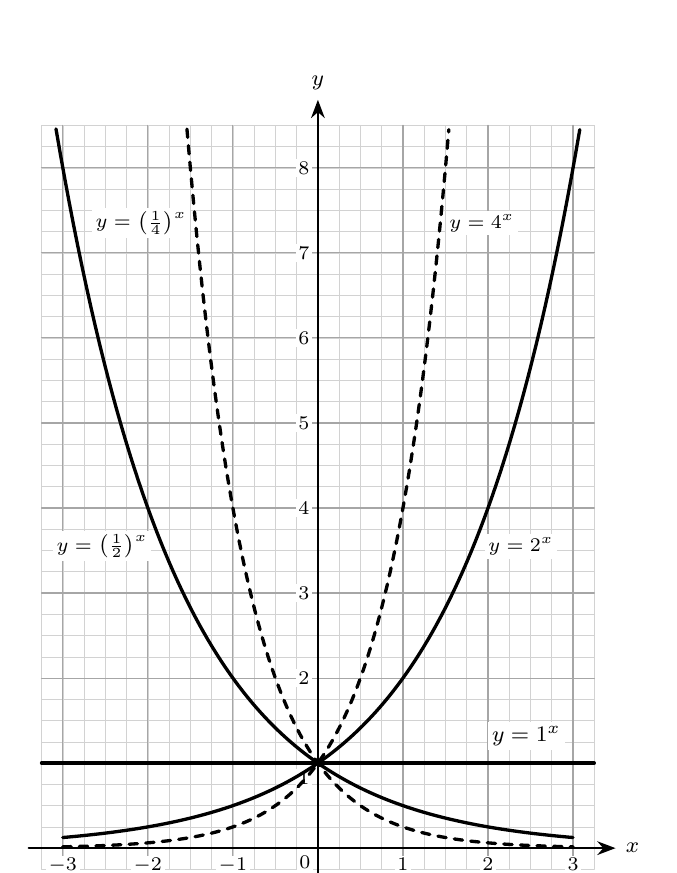
\begin{tikzpicture}[scale=1.08, line cap=round, line join=round, >=Stealth]
    % Grid
    \draw[step=0.25cm, gray!35, very thin] (-3.25, -0.25) grid (3.25, 8.5);
    \draw[step=1cm, gray!70, thin] (-3.25, -0.25) grid (3.25, 8.5);

    % Axes
    \draw[thick, ->] (-3.4, 0) -- (3.5, 0) node[right, font=\footnotesize] {$x$};
    \draw[thick, ->] (0, -0.4) -- (0, 8.8) node[above, font=\footnotesize] {$y$};

    % Axis numbers
    \foreach \x in {-3, -2, -1, 1, 2, 3} {
        \node[below, font=\scriptsize, fill=white, inner sep=1pt] at (\x, -0.08) {$\x$};
    }
    \node[below left, font=\scriptsize, fill=white, inner sep=1pt] at (-0.05, -0.05) {$0$};
    \node[below left, font=\scriptsize, fill=white, inner sep=1pt] at (-0.06, 0.94) {$1$};
    \foreach \y in {2, 3, 4, 5, 6, 7, 8} {
        \node[left, font=\scriptsize, fill=white, inner sep=1pt] at (-0.06, \y) {$\y$};
    }

    % Curves (dashed for base 4 and 1/4, solid for base 2, 1/2, and 1, matching original p. 94)
    % y = 4^x (dashed)
    \draw[very thick, dashed, domain=-3:1.54, samples=120] plot (\x, {pow(4, \x)});
    \node[anchor=west, font=\scriptsize, fill=white, inner sep=1.2pt] at (1.50, 7.35) {$y=4^x$};

    % y = (1/4)^x (dashed)
    \draw[very thick, dashed, domain=-1.54:3, samples=120] plot (\x, {pow(0.25, \x)});
    \node[anchor=east, font=\scriptsize, fill=white, inner sep=1.2pt] at (-1.50, 7.35) {$y=\left(\frac{1}{4}\right)^x$};

    % y = 2^x (solid)
    \draw[very thick, domain=-3:3.08, samples=120] plot (\x, {pow(2, \x)});
    \node[anchor=west, font=\scriptsize, fill=white, inner sep=1.2pt] at (1.96, 3.55) {$y=2^x$};

    % y = (1/2)^x (solid)
    \draw[very thick, domain=-3.08:3, samples=120] plot (\x, {pow(0.5, \x)});
    \node[anchor=east, font=\scriptsize, fill=white, inner sep=1.2pt] at (-1.96, 3.55) {$y=\left(\frac{1}{2}\right)^x$};

    % y = 1^x = 1 (solid)
    \draw[very thick, domain=-3.25:3.25] plot (\x, 1);
    \node[above, font=\footnotesize, fill=white, inner sep=1.5pt] at (2.45, 1.15) {$y=1^x$};
\end{tikzpicture}
\end{center}

\paragraph{【例 3】} $y = f(x) = (\sqrt{2})^{-x}$ 是一個絕對遞減函數。\\
因為由指數的基本性質及 $(\sqrt{2})^0 = 1$，我們有
\[
(\sqrt{2})^{-x} = \frac{1}{(\sqrt{2})^x}.
\]
由【例 2】知道 $(\sqrt{2})^x$ 是絕對遞增函數，所以 $(\sqrt{2})^{-x}$ 是絕對遞減函數。

\paragraph{【例 4】} $y = f(x) = \left(\frac{99}{100}\right)^x$ 是絕對遞減函數。\\
因為 $\frac{99}{100} < 1$，我們有
\[
f(1) < f(0).
\]

\subsubsection*{習題 4-4}

\begin{enumerate}
    \item 試寫出定理 2 遞減情形的詳細證明。
    \item 下面那些函數是遞增的？遞減的？絕對遞增的？絕對遞減的？
    \begin{enumerate}[(i)]
        \item $y = f(x) = x^3$。
        \item $y = f(x) = x^2$。
        \item $y = f(x) = x+5$。
        \item $y = f(x) = -x+7$。
        \item $y = f(x) = [x]$（高斯符號）。
    \end{enumerate}
    \item $y = f(x) = x^2$ 在什麼範圍是遞增的？在什麼範圍是遞減的？
    \item $y = f(x) = (x-1)^2+5$ 在什麼範圍是遞增的？在什麼範圍是遞減的？
    \item 如果 $f(x), g(x)$ 都是遞增的，$f(x)\cdot g(x)$ 是不是遞增的？請討論。
    \item 假設連續函數 $f(x)$ 對一切有理數 $x, y$，滿足 $f(x+y) = f(x)+f(y)$，那麼可以找到一個實數 $c$，使得 $f(x) = cx$。
\end{enumerate}

\subsection{對數函數}\label{sec:b2_4-3}

\subsubsection*{3-1 對數}

在前面我們引入了指數的概念，就是對於正實數 $a$ 與任意實數 $\alpha$，給予符號 $a^\alpha$ 明確的意義。現在我們利用這種概念再介紹一個新的符號如下：

\begin{definition*}
給定一個不等於 1 的正實數 $a$，對於正實數 $b$，如果存在一個實數 $c$，滿足下列關係：
\[
a^c = b,
\]
我們就說 $c$ 是以 $a$ 為底，$b$ 的對數。用符號
\[
\log_a b = c
\]
表示。
\end{definition*}
\paragraph{【討論】}
\begin{enumerate}
    \item 由定義中的條件 $b = a^c$，$b$ 必須是一個正數。所以對數只對於正實數定義，零或負數的對數沒有意義。
    \item 由於指數的性質，對於兩個實數 $c_1, c_2$，我們知道
    \[
    c_1 \neq c_2 \iff a^{c_1} \neq a^{c_2}.
    \]
    成立。因此在定義中對應於 $b$ 的實數 $c$ 是唯一的，所以對數 $\log_a b$ 的定義是明確而有意義的（是一個確定的實數）。
    \item 因為對任意實數 $c,\; 1^c = 1$，在 $a^c = b$ 中，當 $a = 1$ 時，$b$ 非要等於 1 不可，而 $c$ 可以是任意的實數。所以以 1 為底的對數沒有意義。
\end{enumerate}

\paragraph{【例 1】}
\begin{enumerate}[(i)]
    \item $10^2 = 100 \iff \log_{10} 100 = 2$。
    \item $3^5 = 243 \iff \log_3 243 = 5$。
    \item $4^{\frac{1}{4}} = \sqrt{2} \iff \log_4 \sqrt{2} = \frac{1}{4}$。
    \item $2^{10} = 1024 \iff \log_2 1024 = 10$。
    \item $12^2 = 144 \iff \log_{12} 144 = 2$。
    \item $3^{-1} = \frac{1}{3} \iff \log_3 \frac{1}{3} = -1$。
\end{enumerate}

由對數的定義，我們有下面的推論：

\begin{prop}[推論]
設 $a$ 是不等於 1 的正實數，$b$ 是任意正實數，$c$ 是任意實數，那麼我們有
\[
a^{\log_a b} = b, \quad \log_a(a^c) = c.
\]
\end{prop}

\paragraph{【例 2】}
\begin{enumerate}[(i)]
    \item $10^{\log_{10} 100} = 100,\quad \log_{10}(10^2) = 2$。
    \item $3^{\log_3 243} = 243,\quad \log_3(3^5) = 5$。
    \item $4^{\log_4 \sqrt{2}} = \sqrt{2},\quad \log_4(4^{\frac{1}{4}}) = \frac{1}{4}$。
    \item $2^{\log_2 1024} = 1024,\quad \log_2(2^{10}) = 10$。
    \item $12^{\log_{12} 144} = 144,\quad \log_{12}(12^2) = 2$。
    \item $3^{\log_3 \frac{1}{3}} = \frac{1}{3},\quad \log_3(3^{-1}) = -1$。
\end{enumerate}

依據這個推論，$c = \log_a b\; (a, b > 0,\; a \neq 1)$ 就是方程式
\begin{equation}
a^x - b = 0 \label{eq:b2-ch4-ax-minus-b}
\end{equation}
唯一的解。事實上，對於任意正實數 $b$，\eqref{eq:b2-ch4-ax-minus-b} 式必定有解。

\begin{theorem}
給定不等於 1 的正實數 $a$，對於任意正實數 $b$，一定存在一個實數 $c$，滿足 \eqref{eq:b2-ch4-ax-minus-b} 式。
\end{theorem}
\paragraph{【證明】} 假設 $a > 1$（$a < 1$ 時考慮 $a' = \frac{1}{a}$ 即可）。分三種情形討論：
\begin{enumerate}[(i)]
    \item $b = 1$ 時，$c = 0,\; a^0 = 1$。
    \item $b > 1$ 時，我們先求出一個正整數 $k$，使得
    \[
    a^k > b.
    \]
    令 $a_1 = a-1,\; b_1 = b-1$，因 $a > 1, b > 1$，所以 $a_1, b_1$ 是兩個正實數。由上一章 § 3，實數的阿基米德性質，我們知道存在一個正整數 $k$，使得
    \[
    k a_1 > b_1.
    \]
    兩邊同時加 1，得
    \[
    1 + k a_1 > 1 + b_1 = b.
    \]
    又因 $a_1 > 0$ 我們有
    \[
    a^k = (1+a_1)^k > 1 + k a_1 > 1 + b_1 = b,
    \]
    所以
    \[
    a^k > b.
    \]
    設函數 $y = f(x) = a^x$。由假設 $b > 1$ 及以上導出的不等式，就有
    \[
    f(0) < b < f(k).
    \]
    現在由指數函數 $f$ 的連續性，以及連續函數的中間值定理知道，在 0 與 $k$ 之間有實數 $c$ 存在，滿足
    \[
    b = f(c) = a^c.
    \]
    \item $b < 1$ 時，仿照情形 (ii) 中的討論，我們可以求出正整數 $k$，使得 $a^k > \frac{1}{b} > 1$。所以
    \[
    a^{-k} < b < a^0 = 1.
    \]
    同理在 $-k$ 與 0 之間存在實數 $c$，滿足
    \[
    b = f(c) = a^c.
    \]
\end{enumerate}
\hfill〔定理 3 證畢〕

\paragraph{【例 3】}
\begin{enumerate}[(i)]
    \item $2^x - 50 = 0$ 的解 $x$ 在 5 與 6 之間。\\
    因為 $2^5 = 32 < 50 < 2^6 = 64$。
    \item $\left(\frac{15}{10}\right)^x - 2 = 0$ 的解 $x$ 在 1 與 2 之間。\\
    因為 $\frac{15}{10} < 2 < \left(\frac{15}{10}\right)^2 = \frac{225}{100}$。
\end{enumerate}

\subsubsection*{習題 4-5}

\begin{enumerate}
    \item 計算下列各對數之值：
    \begin{enumerate}[(i)]
        \item $\log_4 8$。
        \item $\log_9(\sqrt[3]{3})$。
        \item $\log_8(32^2)$。
        \item $\log_{10}(100^{\frac{1}{3}})$。
        \item $\log 1000^{\frac{1}{10}}$\phantomsection\label{note:b2-ch4-p98-log-base}.
        \item $\log_2(\log_2 16)$。
    \end{enumerate}
    \item 化簡：
    \begin{enumerate}[(i)]
        \item $2^{\log_2 5}$。
        \item $2^{-\log_3 2}$。
        \item $\log_2(2^5)$。
        \item $\log_{10}(10^3)$。
        \item $\log_2(\log_{10} 100)$。
    \end{enumerate}
    \item 化簡下列各式：
    \begin{enumerate}[(i)]
        \item $2^{2\log_2 x}$。
        \item $2^{\log_2 x + \log_2 y}$。
        \item $2^{-\log_2 x}$。
        \item $2^{\log_2 2x - \log_2 y}$。
        \item $2^{2\log_2 x - \log_2 y}$。
    \end{enumerate}
    \item 化簡下列各式：
    \begin{enumerate}[(i)]
        \item $\log_2(4^x)$。
        \item $\log_2(a^{\log_a x})$。
        \item $\log_2(4^x \cdot 2^y)$。
        \item $\log_2(\sqrt{2}\cdot 2^x)$。
    \end{enumerate}
    \item 下列各方程式的解，各在那兩個相鄰的整數之間？
    \begin{enumerate}[(i)]
        \item $2^x - 5 = 0$。
        \item $2^x - \frac{1}{10} = 0$。
        \item $3^x - \frac{1}{10} = 0$。
        \item $2^x - 1000 = 0$。
        \item $3^x - \frac{1}{250} = 0$。
    \end{enumerate}
    \item 
    \begin{enumerate}[(i)]
        \item 試證 $\log_{10} 3$ 不是有理數。
        \item 討論一般的情形，即對於大於 1 的正整數 $a, b$，在什麼情形之下 $\log_a b$ 不是有理數？
    \end{enumerate}
\end{enumerate}

\subsubsection*{3-2 對數的基本特性}

顯然對數的性質與指數的性質間具有密切關係：譬如對應於指數定則 (1), (2)，就有下述對數定則：
\begin{align}
\log_a(uv) &= \log_a u + \log_a v \tag{I}\label{eq:b2-ch4-log-rule-prod} \\
\log_a w &= \log_a c \cdot \log_c w \tag{II}\label{eq:b2-ch4-log-rule-base}
\end{align}
其中 $a, c$ 是不等於 1 的正實數，$u, v, w$ 是任意正實數，\eqref{eq:b2-ch4-log-rule-base} 式又叫做對數換底公式。
\paragraph{【證明】} \eqref{eq:b2-ch4-log-rule-prod} 式的證明留作習題，現在證明 \eqref{eq:b2-ch4-log-rule-base} 式如下：\\
由定理 3 我們可以找到兩個實數 $\alpha, \beta$，使得
\[
c = a^\alpha,\quad w = c^\beta \quad (\text{或 } \alpha = \log_a c,\; \beta = \log_c w).
\]
因此
\[
w = (a^\alpha)^\beta = a^{\alpha\beta}.
\]
所以
\[
\log_a w = \log_a a^{\alpha\beta} = \alpha\beta = \log_a c \cdot \log_c w.
\]
\hfill〔證畢〕

與指數的性質相仿，對數也有下列性質：（$a$ 為正實數）
\begin{equation}
\begin{cases}
\text{如 } a > 1, & \text{則 } b > c \implies \log_a b > \log_a c \\
\text{如 } a < 1, & \text{則 } b > c \implies \log_a b < \log_a c
\end{cases} \tag{III}\label{eq:b2-ch4-log-mono}
\end{equation}

\paragraph{【例 4】} $\log_a u^\alpha = \alpha\log_a u$（$a$ 是不等於 1 的正實數，$u$ 是正實數，$\alpha$ 是任意實數）。\\
\paragraph{【證明】} 設 $\log_a u = b$，就有 $a^b = u$，所以
\[
(a^b)^\alpha = a^{\alpha b} = u^\alpha,
\]
又由對數的定義得到
\[
\log_a u^\alpha = \alpha b = \alpha\log_a u.
\]

\paragraph{【例 5】} $\log_a c = (\log_c a)^{-1}$（$a, c$ 是不等於 1 的正實數）。\\
\paragraph{【證明】} 在公式 \eqref{eq:b2-ch4-log-rule-base} 中，令 $w = a$。

\paragraph{【例 6】} 已知 $\log_{10} 2 = 0.3010$，求 $\log_{10} 5, \log_{10} 40, \log_2 5$。\\
\paragraph{【解】}
\begin{align*}
\log_{10} 5 &= \log_{10} \frac{10}{2} = \log_{10} 10 - \log_{10} 2 \\
&= 1 - 0.3010 = 0.6990. \\
\log_{10} 40 &= \log_{10}(2)^2 + \log_{10} 10 = 2\log_{10} 2 + 1 \\
&= 2\cdot(0.3010) + 1 = 1.6020. \\
\log_2 5 &= \log_2 \frac{10}{2} = \log_2 10 - \log_2 2 \\
&= (\log_{10} 2)^{-1} - 1 = \frac{1}{0.3010} - 1 = \frac{699}{301}.
\end{align*}

\subsubsection*{習題 4-6}

\begin{enumerate}
    \item 證明對數定則 (I)。
    \item 證明 $\log_a \frac{u}{v} = \log_a u - \log_a v$（其中 $a$ 是不等於 1 的正實數，$u, v$ 是任意正實數）。
    \item 證明 $\log_a b \cdot \log_b a = 1$（其中 $a, b$ 是不等於 1 的正實數）。
    \item 下面那些式子是錯的？
    \begin{enumerate}[(i)]
        \item $\log_2(-5) = -\log_2 5$。
        \item $\log_2(3\cdot 5) = \log_2 3 \cdot \log_2 5$。
        \item $\log_2 8 + \log_{\frac{1}{2}} 8 = 0$。
        \item $\log_2(5^3) = (\log_2 5)^3$。
        \item $\log_2(5+3) = \log_2 5 + \log_2 3$。
        \item $\log_2 10 = (\log_{\frac{1}{2}} 10)^{-1}$。
    \end{enumerate}
    \item 求下列各式之值：
    \begin{enumerate}[(i)]
        \item $\frac{1}{2}\log_3 9$。
        \item $\log_4 2 + \log_4 8$。
        \item $3\log_{10} 2 - \log_{10} 80$。
        \item $\log_5 10 - \log_5 \frac{2}{\sqrt{5}}$。
    \end{enumerate}
    \item 令 $\log_2 x = X,\; \log_2 y = Y$，將下列各式以 $X, Y$ 表示：
    \begin{enumerate}[(i)]
        \item $\log_2 xy^2$。
        \item $\log_2 \sqrt{xy}$。
        \item $\log_2 \sqrt{x^3 y}$。
        \item $\log_2 \sqrt[3]{x^5 y^2}$。
    \end{enumerate}
    \item 改正下式右邊的錯誤：
    \[
    \log_2 \sqrt{15} = \frac{1}{2}\log_2 3 + \log_2 5.
    \]
    \item 計算 $\log_2 13 + \frac{1}{2}\log_2 25 + \log_2 \frac{4}{7} - \log_2 \frac{13}{35}$。
    \item $(\log_2 3 + \log_4 9)(\log_3 4 + \log_9 2) = {?}$
    \item $\log_a b \cdot \log_b c \cdot \log_c a = {?}$（$a, b, c$ 是不等於 1 的正數。）
\end{enumerate}

\subsubsection*{3-3 對數函數}

根據前面的定理 3，我們知道，如果 $a$ 是一個不等於 1 的正實數，對數 $\log_a b$ 對於任意正實數 $b$ 都有明確的意義。所以當我們用變數 $x$ 表示一個任意正實數時，$y = f(x) = \log_a x$ 就是一個函數，通常叫做以 $a$ 為底的對數函數。

由定義，對數函數與指數函數有下列關係：
\[
y = \log_a x \iff x = a^y.
\]
由對數的性質，我們直接得到對數函數的性質：
\begin{enumerate}[(i)]
    \item $f(\alpha\beta) = f(\alpha) + f(\beta)$;
    \item $\begin{cases} \text{若 } a > 1, & \text{則 } \alpha > \beta \implies f(\alpha) > f(\beta) \text{（絕對單調遞增）}. \\ \text{若 } a < 1, & \text{則 } \alpha > \beta \implies f(\alpha) < f(\beta) \text{（絕對單調遞減）}. \end{cases}$
\end{enumerate}
對於所有正實數 $\alpha, \beta$ 都成立。反之，任意滿足性質 (i) 的絕對單調函數必定是一個對數函數。

\begin{theorem}
如果 $y = f(x)$ 是一個絕對單調函數而且滿足上述性質 (i)，那麼它一定是一個對數函數。我們可以找到一個適當正實數 $a \neq 1$，使得
\[
f(x) = \log_a x.
\]
\end{theorem}
\paragraph{【證明】} 證明方法與定理 2 相似，請同學們比照研讀。我們考慮單調遞增的情形。由性質 (i) 得到
\[
f(v) = f(1\cdot v) = f(1) + f(v) \implies f(1) = 0.
\]
令 $f(2) = c$，由單調遞增性（即 (ii)）有
\[
c = f(2) > f(1) = 0.
\]
又由 (i) 得
\begin{align*}
f(2^n) &= \underbrace{f(2) + \dots\dots + f(2)}_{n \text{ 項}} = n\cdot f(2) = nc,\quad n \in \mathbb{N}. \\
m\cdot f(2^{\frac{1}{m}}) &= f((\sqrt[m]{2})^m) = f(2) = c. \\
\implies f(2^{\frac{1}{m}}) &= \frac{1}{m}\cdot c,\quad m \in \mathbb{N}. \\
\implies f(2^{\frac{n}{m}}) &= \frac{n}{m}\cdot c,\quad m, n \in \mathbb{N}.
\end{align*}
又
\[
f(2^{-r}) + f(2^r) = f(2^{-r}\cdot 2^r) = f(1) = 0 \implies f(2^{-r}) = -rc \quad (r \in \mathbb{Q}).
\]
所以對於所有有理數 $r \in \mathbb{Q},\; f(2^r) = rc$。從此不難用單調性和極限過程導出
\[
f(2^\beta) = \beta\cdot c
\]
對於所有實數 $\beta \in \mathbb{R}$ 都成立。\\
令 $a = 2^{\frac{1}{c}} > 1$，則有
\begin{align*}
f(a) &= f(2^{\frac{1}{c}}) = \frac{1}{c}\cdot c = 1; \\
f(a^u) &= f((2^{\frac{1}{c}})^u) = f(2^{\frac{u}{c}}) = \frac{u}{c}\cdot c = u.
\end{align*}
但是 $x = a^{\log_a x}$，代入上式就得到
\[
f(x) = f(a^{\log_a x}) = \log_a x.
\]
\hfill〔定理 4 證畢〕\\
單調遞減的情形留作習題。

\paragraph{【例 7】} 設 $a$ 是一個不等於 1 的正實數，則函數 $f(x) = \log_a x$ 與 $g(x) = \log_{\frac{1}{a}} x$ 滿足下列關係：
\[
f(x) = -g(x).
\]
\paragraph{【證明】} 利用 (3-2) 中對數換底公式 (II)，我們有
\[
\log_a x = \log_a \frac{1}{a} \cdot \log_{\frac{1}{a}} x.
\]
但 $\log_a \frac{1}{a} = -1$，所以 $\log_a x = -\log_{\frac{1}{a}} x$，即
\[
f(x) = -g(x).
\]

下圖中作出對數函數 $y = \log_2 x$ 與 $y = \log_{\frac{1}{2}} x$ 的圖形，我們可以看出它們的單調性，以及這種關於 $x$ 軸的對稱關係。

\begin{center}
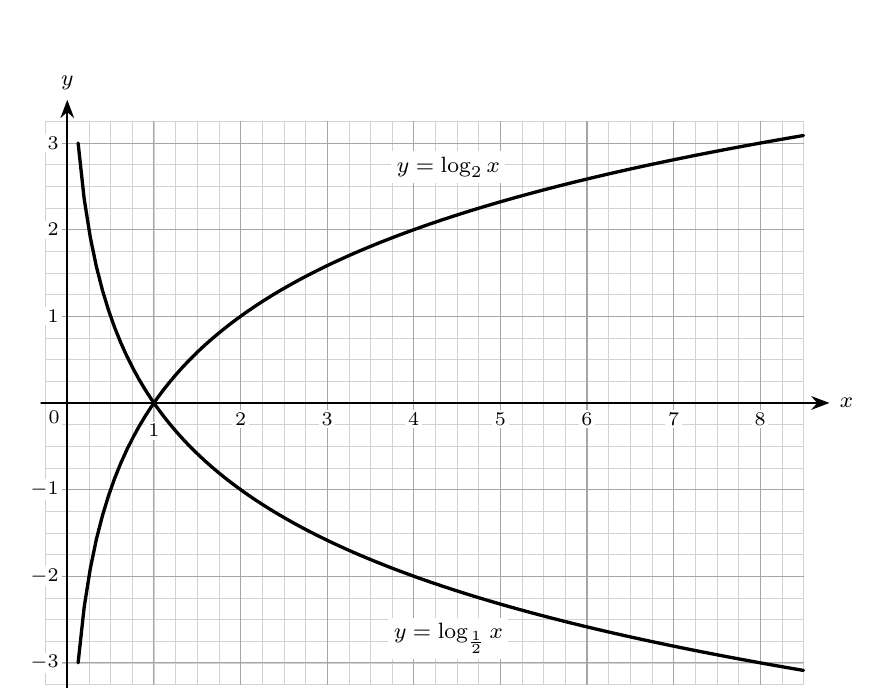
\begin{tikzpicture}[scale=1.1, line cap=round, line join=round, >=Stealth]
    % Grid
    \draw[step=0.25cm, gray!35, very thin] (-0.25, -3.25) grid (8.5, 3.25);
    \draw[step=1cm, gray!70, thin] (-0.25, -3.25) grid (8.5, 3.25);

    % Axes
    \draw[thick, ->] (-0.3, 0) -- (8.8, 0) node[right, font=\footnotesize] {$x$};
    \draw[thick, ->] (0, -3.4) -- (0, 3.5) node[above, font=\footnotesize] {$y$};

    % Axis numbers
    \node[below=5pt, font=\scriptsize, fill=white, inner sep=1pt] at (1, -0.05) {$1$};
    \foreach \x in {2, 3, 4, 5, 6, 7, 8} {
        \node[below, font=\scriptsize, fill=white, inner sep=1pt] at (\x, -0.08) {$\x$};
    }
    \node[below left, font=\scriptsize, fill=white, inner sep=1pt] at (-0.05, -0.05) {$0$};
    \foreach \y in {-3, -2, -1, 1, 2, 3} {
        \node[left, font=\scriptsize, fill=white, inner sep=1pt] at (-0.06, \y) {$\y$};
    }

    % Curves
    % y = log_2(x)
    \draw[very thick, domain=0.125:8.5, samples=120] plot (\x, {ln(\x)/ln(2)});
    \node[font=\footnotesize, fill=white, inner sep=2pt] at (4.4, 2.72) {$y=\log_2 x$};

    % y = log_{1/2}(x)
    \draw[very thick, domain=0.125:8.5, samples=120] plot (\x, {-ln(\x)/ln(2)});
    \node[font=\footnotesize, fill=white, inner sep=2pt] at (4.4, -2.72) {$y=\log_{\frac{1}{2}} x$};
\end{tikzpicture}
\end{center}

\subsubsection*{習題 4-7}

\begin{enumerate}
    \item 已知正數 $x, y$，的和是 8，那麼 $\log_2 x + \log_2 y$ 的最大值是多少？
    \item 當 $2x+5y=20$ 時，試求 $\log_2 x + \log_2 y$ 之最大值。
    \item 設 $x > 2, y > 2$，比較下列各式之大小：
    \[
    \log_2 \frac{x+y}{2}, \quad \frac{1}{2}\log_2(x+y), \quad \frac{1}{2}(\log_2 x + \log_2 y).
    \]
    \item 滿足下列不等式之整數有幾個？
    \[
    0 \le \log_3(\log_3 x) < 1.
    \]
    \item 設 $x > 1, y > 1$，且 $2\log_x y - 2\log_y x + 3 = 0$。那麼 $x^2 - 4y^2$ 的最小值是多少？
    \item 設 $a > 1, b > 1$，試證
    \[
    \log_a b + \log_b a \ge 2.
    \]
    \item 解 $\log_3 x = -2$。
    \item 解 $\log_x 10 = -1$。
    \item 解 $2 = \log_x \frac{1}{4}$。
    \item 解 $\log_{10}(x+1) + \log_{10}(x-2) = 1$。
    \item 解 $\frac{1}{2}\log_{10} 2 + \log_{10} \sqrt{x} = \log_{10}(1+\frac{x}{2})$。
    \item 解
    \[
    \begin{cases}
    \log x + \log y = 2, \\
    x^2 + y^2 = 425.
    \end{cases}
    \]
    \item 解下列各指數方程式：
    \begin{enumerate}[(i)]
        \item $2^x = 3^{x-1}$。
        \item $4.5^{x-1} = 10^{x+1}$。
        \item $7.6^{2x} = 11^{x+3}$。
    \end{enumerate}
\end{enumerate}

\subsection{反函數}\label{sec:b2_4-4}

設 $y = f(x)$ 是由數集 $A$ 到數集 $B$ 的函數，如果對於 $A$ 中任意不同的 $\alpha, \beta$，它們在 $B$ 中的對應數 $f(\alpha), f(\beta)$ 也不相同：
\[
\alpha, \beta \in A,\quad \alpha \neq \beta \implies f(\alpha) \neq f(\beta).
\]
我們就說 $f$ 是嵌射的 (injective) 函數，或者說 $f$ 是個嵌射 (injection)。

\paragraph{【例 1】} 恆等函數 $y = f(x) = x,\; (f: A \to A \text{（其中 $A$ 為任意數集））}$ 是嵌射的。

\paragraph{【例 2】} 線性函數 $y = f(x) = ax+b\; (a\neq 0),\; f: \mathbb{R} \to \mathbb{R}$ 也是嵌射的。

\paragraph{【例 3】} $y = f(x) = x^2,\; f: \mathbb{R} \to \mathbb{R}$ 不是嵌射的（為什麼？），但是 $f: \mathbb{R}^+ \to \mathbb{R}^+$ 是嵌射的，其中 $\mathbb{R}^+$ 是所有正實數的集合。

由絕對單調的意義，絕對單調函數是嵌射的，所以指數函數與對數函數都是嵌射的。

\subsubsection*{習題 4-8}

下列函數各在那些範圍是嵌射的？
\begin{enumerate}
    \item $y = f(x) = x^3$。
    \item $y = f(x) = x^n,\; n$ 是正整數。
    \item $y = f(x) = \sqrt{x}$。
    \item $y = f(x) = |x|$。
    \item $y = f(x) = [x]$（高斯符號）。
    \item $y = f(x) = \log_2 x^2$。
\end{enumerate}

我們現在來討論函數的另一種性質。考慮由 $A$ 到 $B$ 的函數 $y = f(x)$，如果 $B$ 中每一個數 $b$ 在函數 $f$ 的作用下，都是 $A$ 中某一個數或某些數的對應數；也就是說：
\[
\text{對於任意 } b \in B\text{，存在至少一個 } a \in A\text{，使得 } b = f(a).
\]
這樣我們就說：$f$ 是由 $A$ 到 $B$ 的蓋射 (surjcetion)\phantomsection\label{note:b2-ch4-p106-surjcetion} 或 $f$ 是個由 $A$ 到 $B$ 的蓋射的 (surjective) 函數。

由 $A$ 到 $B$ 的一個函數 $y = f(x)$，如果同時又是蓋射的，又是嵌射的，就叫對射的 (bijective)，或者 $f$ 叫做一個由 $A$ 到 $B$ 的對射 (bijection)。

\paragraph{【例 4】} 例一、例二中的恆等函數與線性函數都是由 $\mathbb{R}$ 到 $\mathbb{R}$ 的對射。

\paragraph{【例 5】} 指數函數是由 $\mathbb{R}$ 到 $\mathbb{R}$ 的嵌射而不是蓋射，所以也不是對射的。而對數是由 $\mathbb{R}^+$ 到 $\mathbb{R}$ 的對射。

\paragraph{【例 6】} 但指數函數是由 $\mathbb{R}$ 到 $\mathbb{R}^+$（正實數的集合）的對射。由此可知嵌射，對射，蓋射等觀念和集 $A, B$ 有關。

\begin{theorem}
如果 $f$ 是由數集 $A$ 到數集 $B$ 的對射，那麼必存在一個唯一的由 $B$ 到 $A$ 的對射 $g$，使得
\[
f(a) = b \iff g(b) = a,\quad (a \in A, b \in B).
\]
也就是說
\[
f(g(b)) = b,\quad g(f(a)) = a.
\]
\end{theorem}

\begin{definition*}
上面定理中的函數 $g$ 叫做 $f$ 的反函數（或逆函數），用符號 $f^{-1}$ 表示，不難看出 $f$ 也是 $g$ 的反函數。所以 $f$ 與 $g$ 互為反函數。
\[
(g = f^{-1},\; f = g^{-1} = (f^{-1})^{-1}).
\]
\end{definition*}
\paragraph{【證明】（定理 5）} 對於任意 $b \in B$，由 $f$ 的蓋射性質，知道存在至少一個 $a \in A$，使得 $f(a) = b$，而且由於 $f$ 的嵌射性質，知道這樣的 $a$ 最多只有一個。因此我們很自然的可以作一個由 $B$ 到 $A$ 的對應：$b \longrightarrow a$，這樣的對應很顯然的是一個由 $B$ 到 $A$ 的函數，這就是我們所要求的函數 $g$。\\
$g$ 是嵌射的，因為對於 $b_1, b_2 \in B$，
\[
g(b_1) = g(b_2) = a \in A \implies f(a) = b_1,\; f(a) = b_2 \implies b_1 = b_2.
\]
$g$ 是蓋射的，因為對於任意 $a \in A,\; f(a) = b \in B$，就有
\[
g(b) = a.
\]

\paragraph{【例 7】} 恆等函數 $f: A \to A$ 的反函數 $f^{-1} = f$。

\paragraph{【例 8】} 線性函數 $f(x) = ax+b\; (a\neq 0)$ 的反函數是
\[
f^{-1}(x) = \frac{1}{a}x - \frac{b}{a}.
\]
辦法很簡單，我們由 $y = ax+b,\; a\neq 0$ 來反解 $x$，得到
\[
x = \frac{1}{a}y - \frac{b}{a},\quad \text{並把它寫做 } f^{-1}(y). \text{ 所以}
\]
\[
f^{-1}(x) = \frac{1}{a}x - \frac{b}{a}.
\]

\begin{prop}[推論 1]
如果 $f$ 是由數集 $A$ 到數集 $B$ 的絕對遞增（遞減）蓋射的函數，那麼反函數 $f^{-1}$ 存在，而且是由 $B$ 到 $A$ 的絕對遞增（遞減）蓋射的函數。
\end{prop}
\paragraph{【證明】} 由上面定理，知道反函數 $f^{-1}$ 存在，而且是一個由 $B$ 到 $A$ 的對射，對於 $f^{-1}$ 的絕對單調性，我們不妨假設 $f$ 是遞增的。\\
如果 $b_1, b_2 \in B$，而且 $b_1 < b_2$，設 $a_1 = f^{-1}(b_1),\; a_2 = f^{-1}(b_2)$，那麼 $f(a_1) = b_1,\; f(a_2) = b_2$，如果 $a_1 \ge a_2$，由 $f$ 的絕對遞增性質，知道 $b_1 = f(a_1) \ge f(a_2) = b_2$，與 $b_1 < b_2$ 的假設矛盾，因此 $a_1 < a_2$，即
\[
b_1 < b_2 \implies f^{-1}(b_1) < f^{-1}(b_2).
\]

\begin{prop}[推論 2]
設 $a$ 為不等於 1 的正實數，則以 $a$ 為底的指數函數 $y = f(x) = a^x,\; f: \mathbb{R} \to \mathbb{R}^+$（正實數的集合），與對數函數 $x = g(y) = \log_a y,\; g: \mathbb{R}^+ \to \mathbb{R}$ 互為反函數。
\end{prop}

\begin{theorem}
如果 $f$ 是一個由區間 $[a, b]$ 到區間 $[c, d]$ 的對射的連續函數，那麼 $f$ 是絕對單調函數。
\end{theorem}
\paragraph{【證明】} 不妨假設 $f(a) < f(b)$，我們要證明 $f$ 是絕對遞增。對於 $(a, b)$ 中任意數 $a_1$，如果
\[
f(a_1) < f(a) < f(b),
\]
那麼由 $f$ 在區間 $[a, b]$ 上的連續性與連續函數的中間值定理，在 $(a_1, b)$ 中必定存在一個數 $b_1$，使得
\[
f(b_1) = f(a).
\]
這和 $f$ 的嵌射性質不合，又如果 $f(a) < f(b) < f(a_1)$，那麼在 $(a, a_1)$ 中必定存在一個數 $b_2$，使得
\[
f(b_2) = f(b).
\]
又得到矛盾，所以
\[
f(a) < f(a_1) < f(b).
\]
現在對於任意兩數 $a_1, a_2;\; a < a_1 < a_2 < b$，由以上的討論，我們知道 $f(a) < f(a_2)$。把 $a_2$ 代替上面的討論中的 $b$，就得到 $f(a) < f(a_1) < f(a_2)$。綜合以上結果：
\[
a \le a_1 < a_2 \le b \implies f(a_1) < f(a_2).
\]
在這種情形下，顯然 $f(a) = c,\; f(b) = d$，當然在遞減的情形，就有 $f(a) = d,\; f(b) = c$。

\begin{theorem}
在定理 6 的假設下，$f$ 的反函數 $f^{-1}$ 存在，而且也是連續的。
\end{theorem}
\paragraph{【證明】} 如果 $f$ 是絕對遞增的，由推論 1 知道 $f^{-1}$ 存在而且是絕對遞增的。設 $y_0$ 是 $c, d$ 之間的一個任意數，任意選取一個遞增，一個遞減的數列 $\langle y_n \rangle, \langle y'_n \rangle$ 逼近 $y_0$。
\[
y_1 < y_2 < \dots\dots < y_n < \dots\dots < y_0 < \dots\dots < y'_n < \dots\dots < y'_2 < y'_1.
\]
並且
\[
y_0 = \lim_{n\to\infty} y_n = \lim_{n\to\infty} y'_n,\quad \lim_{n\to\infty}(y'_n - y_n) = 0.
\]
設 $x_0 = f^{-1}(y_0),\; x_n = f^{-1}(y_n),\; x'_n = f^{-1}(y'_n),\; n=1, 2, 3, \dots$，由 $f^{-1}$ 的單調遞增性得到
\[
x_1 < x_2 < \dots\dots < x_n < \dots\dots < x_0 < \dots\dots < x'_n < \dots\dots < x'_2 < x'_1.
\]
我們只要證明 $\lim_{n\to\infty}(x'_n - x_n) = 0$，也就是說
\[
\lim_{n\to\infty} x_n = x_0 = \lim_{n\to\infty} x'_n.
\]
如果不然，假設 $\lim_{n\to\infty} x_n \neq x_0$，那麼一定存在一個數 $a_1$：
\[
x_n < a_1 < x_0,\quad x = 1, 2, 3, \dots\dots\phantomsection\label{note:b2-ch4-p109-index-x}
\]
由函數 $f$ 的單調遞增性得到
\[
y_n < c_1 = f(a_1) < y_0,\quad n=1, 2, 3, \dots\dots
\]
但是這和 $\lim_{n\to\infty} y_n = y_0$ 互相矛盾，因此 $\lim_{n\to\infty} x_n = x_0$；\\
同理可證 $\lim_{n\to\infty} x'_n = x_0$。

由指數函數的連續性與定理 7，我們得到下面的推論。

\begin{prop}[推論]
對數函數 $y = f(x) = \log_a x$（$a$ 是一個不等於 1 的正實數）是連續函數。
\end{prop}

\subsubsection*{習題 4-9}

\begin{enumerate}
    \item 設 $f(x) = 2x-3, g(x) = x-1$ 為兩個多項式函數。
    \begin{enumerate}[(i)]
        \item 試求 $g[f(x)]$（這叫做函數 $f$ 與 $g$ 的合成函數，通常用符號 $g\circ f(x)$ 表示，亦即 $g\circ f(x) = g[f(x)]$）。
        \item 試證 $f$ 與 $g$ 都是對射，並求其反函數 $f^{-1}$ 與 $g^{-1}$。
    \end{enumerate}
    \item 設 $f(x) = \frac{1}{2}(a^x + a^{-x}),\; g(x) = \frac{1}{2}(a^x - a^{-x})$。\\
    試證 $f(x+y) = f(x)f(y) + g(x)g(y)$。
    \item 求函數 $y = \log_2(x-2)$ 的反函數。
    \item 求函數 $y = \log_2 \frac{1}{x}$ 的反函數。
    \item 求函數 $y = 2^{-2x}$ 的反函數。
    \item 對於下列各函數，分別找出最大的實數集合 $A, B$，使得函數 $f$ 成為自 $A$ 到 $B$ 的對射：
    \begin{enumerate}[(i)]
        \item $y = f(x) = x^2$。
        \item $y = f(x) = \sqrt{2x+1}$。
        \item $y = f(x) = x^3$。
        \item $y = f(x) = \log_2 |x|$。
        \item $y = f(x) = \log_2(1+x^2)$。
        \item $y = f(x) = 2^{1+2x}$。
        \item $y = f(x) = 2^{-|x|}$。
    \end{enumerate}
\end{enumerate}
 % 第四章 指數函數與對數函數
% =========================================================================
% 《高中數學實驗教材》第二冊（高一下） 
% 第五章 對數表的用法與計算尺原理*
% =========================================================================

\section{對數表的用法與計算尺原理\texorpdfstring{$^*$}{*}}\label{sec:b2_ch5}

\subsection{對數表}

在算術四則的計算裏，加減比乘除要簡單多了——尤其是有一堆很大的數目字的時候，更是如此。（不信，你就計算 $3.2705319 \times 927.6412195$ 和 $3.2705319 + 927.6412195$ 比較看看！）即使我們只想得到一個近似值，乘除也會比加減麻煩得多。

對數函數的發明和對數函數表的利用，就是使我們能夠將乘除的計算改成加減的，並且使它器械化！

假設 $a$ 是一個不等於 1 的正數，而且用 $a$ 做底的對數函數已經編列成表，也就是說對任一個正數 $x$，$\log_a x$ 一查便知，而它的反函數卽指數函數 $a^x$，也一查便知。那麼要知道兩個正數 $x, y$ 的乘積 $xy$，只需先知道 $\log_a xy$，剩下就只要查表了。（動眼睛不動手！）

但因為
\[
\log_a xy = \log_a x + \log_a y,
\]
我們只需先查出 $\log_a x$ 和 $\log_a y$，做加法運算（只有在這裏要動手！），就得到 $\log_a xy$ 了！\footnote{計算尺之使用不在部頒課程標準之內，但其原理極其簡單，爲對數計算之一應用而已，並且在實際計算時使用計算尺極為方便，高中同學皆應了解計算尺原理及簡單使用方法，並可在物理學、化學課程中使用。如因教學時間限制，亦可略去不講，留供同學自行參考。}

同樣的道理要計算 $z = \frac{xy}{uvw}$（設 $x, y, u, v, w$ 都是正數），我們可以這麼做：
\begin{enumerate}[(1)]
    \item 查表得出 $\log_a x, \log_a y, \log_a u, \log_a v, \log_a w$。
    \item 算出 $S = \log_a x + \log_a y - \log_a u - \log_a v - \log_a w$。
    \item 查表找出正數 $z$ 使得 $\log_a z = S$。
\end{enumerate}

\paragraph{【例 1】} 求
\[
\frac{3.67 \times 4.92 \times 7.25}{9.75 \times 8.73}
\]

\paragraph{【解】}
\begin{align*}
\text{查表得} \qquad \log_{10} 3.67 &= 0.5647 & \log_{10} 9.75 &= 0.9890 \\
\log_{10} 4.92 &= 0.6920 & +\;)\; \log_{10} 8.73 &= 0.9405 \\
\cline{4-4}
+\;)\; \log_{10} 7.25 &= 0.8603 & & 1.9295 \\
\cline{2-2}
& 2.1170
\end{align*}
\[
2.1170 - 1.9295 = 0.1875.
\]
\[
\log_{10} 1.54 = 0.1875. \qquad \therefore \text{答案是 } 1.54.
\]

通常用的對數表只有兩種，一種是用 10 做底數的，叫做「常用」對數表。一種是用一個特別重要的數 $e = 2.71828\dots\dots$ 作底數的，叫做「自然」對數表，後者特別在高等數學裏有極重要的理論價值，但是我們現在只對常用對數有興趣，因此以下就用 $\log$ 代替 $\log_{10}$。

為什麼 10 是最實用的對數呢？這是因爲人類用慣了十進位制的原故。由公式 $\log xy = \log x + \log y$，我們的對數表只需列上區間 $1 < x < 10$ 裏的 $x$ 的對數，譬如說
\begin{align*}
\log 497 &= \log(100 \times 4.97) \\
&= \log 100 + \log 4.97 = 2 + 0.6964 \\
&= 2.6964.
\end{align*}
而 $\log 0.0000497 = -5 + 0.6964 = -4.3036$。

在對數表所列的對數值幾乎全是近似值，因此我們在計算時一定得有近似值計算法的常識。我們特別提到下面兩點：

\subsubsection{精確度}

每個正數 $a$ 都可以化成一個 10 的倍數與個位數的乘積。卽存在整數 $k$ 使得 $1 \le \frac{a}{10^k} < 10$，所以
\[
a = \left(\frac{a}{10^k}\right) 10^k.
\]
這叫做標準寫法（或科學記法）。

若取 $a$ 的對數，就得到 $k = [\log a]$，卽 $\log a$ 的整數部分。另一方面，我們說 $\frac{a}{10^k}$ 是 $a$ 的有效數字部分，它的長度，亦卽 $\frac{a}{10^k}$ 的小數點下位數加 1，就叫 $a$ 的有效數字位數。

例如 $0.0000437$ 的有效數字是 $4.37$，有三位有效數字，而 $\log 0.0000437$ 的整數部分爲 $-5$，所以 $0.0000437$ 的標準寫法是
\[
4.37 \times 10^{-5}.
\]

在計算近似值時，我們必須指明精確到幾位有效數字。例如 $0.09235716$ 若取三位有效數字的精確度，我們就寫成：
\[
9.24 \times 10^{-2}
\]
若是 $70,454,620,000$ 取四位有效數字的精確度就寫成
\[
7.045 \times 10^{10}.
\]

\paragraph{注意：} 前面例子有效數字中，最後一位數字都已經過四捨五入的處理了，如果最後一例中，取二位數字的精確度就要寫作
\[
7.0 \times 10^{10},
\]
不可以寫作 $7 \times 10^{10}$！

在一長串的乘除中，所得結果的精確度的位數不會大過各乘除因子精確度位數的最小者。這是我們最須緊記的一點！很多人最常患的錯誤是對一串乘積中的某一個因子苛刻地求其精確度，（例如精確到八，九位有效數字），而沒有考慮到當別的因子精確度太差時（例如只精確到三，四位），這種苛求就完全失去意義了。

\paragraph{【例 2】} $4.128 \times 2.953 = 12.189$\phantomsection\label{note:b2-ch5-p114-ex2}

\subsubsection*{習題 5-1}
\begin{enumerate}
    \item 某棟樓八十幾萬元，某乙說某物一斤值幾十元，兩個人誰比較沒有科學觀念？
    \item 已知 $47^{100}$ 爲 168 位數；試問 $47^{17}$ 爲幾位數？
    \item 氫原子的質量是 $0.000,000,000,000,000,000,000,001,6734\text{g}$（克），如何寫成標準形式。
    \item 求下列各對數：
    \begin{enumerate}[(i)]
        \item $\log \frac{1}{3.5 \times 2.64}$,
        \item $\log \frac{5070000}{2}$,
        \item $\log \frac{8.59 \times 9.75}{4.15}$,
    \end{enumerate}
    \item 利用對數算出下列各數的近似值至二位小數
    \begin{enumerate}[(i)]
        \item $\frac{3.99 \times 3.69}{4}$,
        \item $1530000 \times 0.0086$,
        \item $0.00251 \times 0.000379$,
    \end{enumerate}
\end{enumerate}

從實用的立場來說，對數表給出四位小數就已夠用了！另一個和表的精確度密切相關的觀念是表的細密度，像我們書後附錄的對數表就細密到三位有效數字，因爲對數表不可能把每個 1 到 10 之間的 $x$（$1 \le x < 10$）的對數 $\log x$ 都列出，例如表上沒有 $\log 7.4142$，只有 $\log 7.41, \log 7.42, \log 7.43$ 等等。所以要計算 $\log 7.4142$ 就要用內插法。

\subsubsection{內插法查表}

就拿 $\log 7.4142$ 來討論：

\begin{center}
\renewcommand{\arraystretch}{1.2}
\begin{tabular}{c|c}
$x$ & $y = \log x$ \\ \hline
$7.42$ & $0.8704$ \\
$7.41$ & $0.8698$ \\ \hline
\text{差 } $\Delta x = 0.01$ & $\Delta y = 0.0006$
\end{tabular}
\end{center}

這 0.0006 是相當於 $x$ 自 7.41 變到 7.42 時 $y = \log x$ 的變化。

我們自然想問：如果 $x$ 自 7.41 變到 7.4142，$y$ 會變爲多少？

內插法的原理是：在一個很小的範圍內來說，$x$ 的微差和 $y$ 的微差近似地成比例。在此來說，就是對 $y = \log 7.4142$，我們可以有：\phantomsection\label{note:b2-ch5-p115-interpolation-zero}
\begin{align*}
(y - 0.8698) : (7.4142 - 7.41) &= (0.8704 - 0.8698) : (7.42 - 7.41) \\
&= 0.0006 : 0.01 \\
y &= 0.8698 + 0.006 \cdot \frac{0.0042}{0.01} \\
&= 0.8698 + 0.000252 \\
&= 0.8701. \qquad\quad \text{答 } \log 7.4142 = 0.8701.
\end{align*}

讓我們再註解一下：0.0042 中的 2 不值得考慮，因爲這種精度不太有意義，所以如果答案寫作 0.8700 也未嘗不可，最後一位的誤差，完全在意料之中。

同學們請注意，比例內插法的校正數值表，通常就附在對數表內。例如求 $\log 7.418$，查對數表得
\[
\log 7.41 = 0.8698
\]
$\Delta x = 7.418 - 7.41 = 0.008$，查所附校正數值表（對數表中最後三欄）讀出校正數值 $\Delta y = 0.0005$，所以
\[
\log 7.418 = 0.8698 + 0.0005 = 0.8703.
\]

\subsubsection*{習題 5-2}
\begin{enumerate}
    \item 比例內插法在圖解法上有什麼意義？
    \item 求下列對數：
    \begin{enumerate}[(i)]
        \item $\log 1024$,
        \item $\log 1547000$,
        \item $\log 0.000007698$,
        \item $\log 98690$,
        \item $\log 0.085741$。
    \end{enumerate}
\end{enumerate}

對數表 $\log x$ 中的 $x$ 都在 1 與 10 之間，因此 $\log x$ 都是介於 0 和 1 間的小數，而一般個位數以上的情形如：
\[
\log 7.41 = 0.8698, \; \log 74.1 = 1.8698 \text{ 及 } \log 7410 = 3.8698, \text{ 等等。}
\]
因此，爲一致且方便起見，對於小數的對數計算，都把 $\log 0.00741 = -3 + 0.8698$，記作 $\bar{3}.8698$；如果你眞去算出 $\log 0.00741 = -2.1302$，那常會是畫蛇添足，因為取對數值多半只是運算中的過程而不是目的。

\paragraph{【例 3】} $8.85 \times 0.762 \div 0.04796 = ?$

\paragraph{【解】}\phantomsection\label{note:b2-ch5-p116-ex3-minus-log}
\begin{align*}
\log 8.85 &= 0.9469, \\
\log 0.762 &= \bar{1}.8820 \\
-\quad \log 0.04796 &= 1.3192 \\
\cline{1-2}
\log ? &= 2.1481.
\end{align*}
\[
(\log 0.04796 = \bar{2}.6808)
\]
查表知 $\log 1.40 = 0.1461$。
\[
\Delta x \sim 0.007, \quad \Delta y = 21
\]
\[
\therefore \text{答案是 } 140.7.
\]

\paragraph{【例 4】} 求 $x = \sqrt[5]{0.00626}$

\paragraph{【解】}
\[
\log x = \frac{1}{5} \log 0.00626 = \frac{1}{5} (\bar{3}.7966)
\]
\[
= -0.6 + 0.15932 = \bar{1}.5593
\]
查表知
\[
\log 0.362 = \bar{1}.5587
\]
\[
\Delta y = 5593 - 5587 = 6,
\]
查校正數值表得
\[
\Delta x = 0.0005.
\]
\[
\text{答 } x = 0.3625.
\]

\paragraph{【例 5】} $u = \frac{4}{3} \pi \times 0.875^3$

\paragraph{【解】}
\begin{align*}
\log \pi &= 0.4971 & \log 3 &= 0.4771 \\
\log 4 &= 0.6021 & \log 0.875 &= \bar{1}.9420 \\
+\qquad & \bar{1}.3489 & \log 0.875^3 &= \bar{1}.8260 \\
\cline{1-2}
\log u &= 0.4481 & -0.4771 \\
\cline{3-4}
\log 2.80 &= 0.4472 & & \bar{1}.3489
\end{align*}
\[
\Delta y = 4481 - 4472 = 9,
\]
查出 $\Delta u = 0.006$
\[
\text{答 } u = 2.806.
\]

\subsubsection*{習題 5-3}
\begin{enumerate}
    \item 下列各數是那些數的對數？
    \begin{enumerate}[(i)]
        \item $2.7157$,
        \item $\bar{2}.7157$,
        \item $-2.7157$,
        \item $0.6990 + \bar{1}.5445 - 2.3098$,
        \item $\bar{1}.7082 + \bar{2}.4771 - \bar{3}.6021$。
    \end{enumerate}
    \item 求 $\sqrt[3]{0.5495}$。
    \item 求 $5.42 \times 3.5 \times 2.55 \div 8.12$。
    \item 求 $(9.29 \times 10^3)^5$。
    \item 利用對數求 $2^{10}$。
    \item 求正整數 $n$ 使 $4000 < (\frac{5}{4})^n < 5000$，利用 $\log_{10} 2 = 0.3010$。
    \item 已知 $\log 3 \fallingdotseq 0.4771$。問 $(\frac{1}{3})^{20}$ 表成小數時，不等於 0 的第 1 個數字出現在那裏？
    \item 
    \begin{enumerate}[(i)]
        \item 求最小整數指數 $x$，使 $(\frac{4}{5})^x < 0.000001$；
        \item 求最小整數指數 $x$，使 $(\frac{3}{5})^x < 0.0001$。
    \end{enumerate}
    \item 
    \begin{enumerate}[(i)]
        \item 求最小整數指數 $x$，使 $(\frac{10}{9})^x > 1000000$；
        \item 求最小整數指數 $x$，使 $(\frac{9}{8})^x > 10000000$。
    \end{enumerate}
\end{enumerate}

\subsection{計算尺原理\texorpdfstring{$^*$}{*}}

上面已經說明如何利用對數和對數表把乘除化爲加減，也把乘方化爲倍數的（近似值）計算法。這個辦法更可以和圖表或者器械配合起來使用，其中最重要最具實用價值的就是計算尺。\footnote{見 111 頁之說明。}

式子 $\log xy = \log x + \log y$，在器械上很容易表達出來：

\begin{center}
\begin{tikzpicture}[scale=1.0, line cap=round, line join=round, >=Stealth]
    % --- Figure 1 (Left) ---
    \begin{scope}[shift={(0, 0)}]
        \draw[thick, |-|] (0, 1.45) -- (2.5, 1.45) node[midway, above=2pt] {\small $\log x$};
        \draw[thick, |-|] (2.5, 0.75) -- (3.8, 0.75) node[midway, above=2pt] {\small $\log y$};
        \draw[thick, |-|] (0, 0.05) -- (3.8, 0.05) node[midway, above=2pt] {\small $\log xy$};
        \node at (1.9, -0.75) {\small 圖\quad 1};
    \end{scope}
    
    % --- Figure 2 (Right) ---
    \begin{scope}[shift={(4.8, 0)}]
        % Box (taller for clean internal labels)
        \draw[thick] (0, 0) rectangle (9.2, 1.65);
        
        % Top linear scale: 0 to 1, width 9.2cm
        \foreach \i in {0, 1, 2, 3, 4, 5, 6, 7, 8, 9, 10} {
            \pgfmathsetmacro{\xpos}{\i * 0.92}
            \draw (\xpos, 1.65) -- (\xpos, 1.50);
            \ifnum\i=0
                \node[above=2pt] at (\xpos, 1.65) {\scriptsize 0};
            \else\ifnum\i=10
                \node[above=2pt] at (\xpos, 1.65) {\scriptsize 1};
            \else
                \node[above=2pt] at (\xpos, 1.65) {\scriptsize 0.\i};
            \fi\fi
        }
        
        % Bottom log scale: k = 1 to 10
        \foreach \k in {1, 2, 3, 4, 5, 6, 7, 8, 9, 10} {
            \pgfmathsetmacro{\xpos}{9.2 * log10(\k)}
            \draw (\xpos, 0) -- (\xpos, 0.15);
            \node[below=2pt] at (\xpos, 0) {\scriptsize \k};
        }
        % Position for x cleanly centered between 5 and 6
        \pgfmathsetmacro{\xval}{5.48}
        \pgfmathsetmacro{\xposx}{9.2 * log10(\xval)}
        \draw (\xposx, 0) -- (\xposx, 0.15);
        \node[below=2pt] at (\xposx, 0) {\scriptsize $x$};
        
        % Dashed lines and internal arcs (no overlap with top scale numbers)
        \pgfmathsetmacro{\xposthree}{9.2 * log10(3)}
        \draw[densely dashed] (\xposthree, 0) -- (\xposthree, 1.65);
        \node[anchor=west, font=\scriptsize, fill=white, inner sep=1pt] at ({\xposthree + 0.08}, 1.20) {$0.4771$};
        \draw[densely dashed] (0, 1.65) .. controls (1.2, 1.18) and (3.2, 1.18) .. (\xposthree, 1.65)
            node[midway, fill=white, inner sep=1.2pt, font=\scriptsize] {$\log 3$};
        
        % log x: deeper dashed curve to x
        \draw[densely dashed] (\xposx, 0) -- (\xposx, 1.65);
        \draw[densely dashed] (0, 1.65) .. controls (2.2, 0.38) and (4.8, 0.38) .. (\xposx, 1.65)
            node[pos=0.45, fill=white, inner sep=1.2pt, font=\scriptsize] {$\log x$};
        
        \node at (4.6, -0.75) {\small 圖\quad 2};
    \end{scope}
\end{tikzpicture}
\end{center}

所以要計算乘法，最好是用「對數尺度」。這就是說，我們在一根尺上，在離原點長爲 $\log x$ 的地方刻上 $x$，如圖 2. 那麼上述的圖，就變成了圖 3：

\begin{center}
\begin{tikzpicture}[scale=1.1, line cap=round, line join=round]
    \draw[thick, |-|] (0, 1.3) -- (2.6, 1.3) node[midway, above] {$x$};
    \draw[thick, |-|] (2.6, 0.65) -- (3.9, 0.65) node[midway, above] {$y$};
    \draw[thick, |-|] (0, 0) -- (3.9, 0) node[midway, above] {$x\,y$};
    
    % Guide alignment lines
    \draw[gray, thin] (0, 1.3) -- (0, 0);
    \draw[gray, thin] (2.6, 1.3) -- (2.6, 0.65);
    \draw[gray, thin] (3.9, 0.65) -- (3.9, 0);
    
    \node at (1.95, -0.6) {圖\quad 3};
\end{tikzpicture}
\end{center}

這個運作只需要兩根對數尺度就夠了。最簡單的計算尺正面通常如圖 5 由上中下三板構成，上下兩塊長板完全固定起來，分別叫上下定板，而中間的卻可以活動，叫遊板。依慣例，下面的板上一定有「D 尺」，而中間的長板的最下方一定刻有「C 尺」。 C 尺和 D 尺在刻劃上完全一樣是用對數尺度。

如果 C 尺上的 $a, b$ 點對齊 D 尺上的 $c, d$ 點（見圖 4），則由
\[
\log b - \log a = \log d - \log c
\]
就得到
\[
\frac{b}{a} = \frac{d}{c}.
\]

\begin{center}
\begin{tikzpicture}[scale=1.0, line cap=round, line join=round, >=Stealth]
    % Upper strip: C scale, width 6.5, shifted by 1.2
    \draw[thick, rounded corners=2pt] (1.2, 0.70) rectangle (7.7, 1.40);
    \node[right] at (1.28, 1.05) {\footnotesize\textbf{C}};
    \node at (1.85, 1.05) {\footnotesize $1$};
    \node[left] at (7.60, 1.05) {\footnotesize $10$};
    
    % Lower strip: D scale, width 6.5, at x = 0
    \draw[thick, rounded corners=2pt] (0, 0) rectangle (6.5, 0.70);
    \node[right] at (0.08, 0.35) {\footnotesize\textbf{D}};
    \node at (0.65, 0.35) {\footnotesize $1$};
    \node[left] at (6.40, 0.35) {\footnotesize $10$};
    
    % Alignment ticks and labels cleanly inside strips
    \draw (1.85, 0.70) -- (1.85, 0.80); % 1 on C
    \draw (0.65, 0.70) -- (0.65, 0.60); % 1 on D
    \draw (3.1, 0.60) -- (3.1, 0.80);
    \draw (5.3, 0.60) -- (5.3, 0.80);
    
    \node at (3.1, 1.05) {\footnotesize $a$};
    \node at (5.3, 1.05) {\footnotesize $b$};
    \node at (3.1, 0.35) {\footnotesize $c$};
    \node at (5.3, 0.35) {\footnotesize $d$};
    
    % Vertical dashed extension lines strictly outside strips (no strike-through)
    \draw[densely dashed] (1.85, 1.40) -- (1.85, 2.35);
    \draw[densely dashed] (3.1, 1.40) -- (3.1, 1.92);
    \draw[densely dashed] (5.3, 1.40) -- (5.3, 2.35);
    
    \draw[densely dashed] (0.65, 0) -- (0.65, -0.95);
    \draw[densely dashed] (3.1, 0) -- (3.1, -0.52);
    \draw[densely dashed] (5.3, 0) -- (5.3, -0.95);
    
    % Dimension arrows above C with white-backed labels
    \draw[<->] (1.85, 1.78) -- (3.1, 1.78) node[midway, fill=white, inner sep=1.5pt, font=\scriptsize] {$\log a$};
    \draw[<->] (1.85, 2.24) -- (5.3, 2.24) node[midway, fill=white, inner sep=1.5pt, font=\scriptsize] {$\log b$};
    
    % Dimension arrows below D with white-backed labels
    \draw[<->] (0.65, -0.38) -- (3.1, -0.38) node[midway, fill=white, inner sep=1.5pt, font=\scriptsize] {$\log c$};
    \draw[<->] (0.65, -0.84) -- (5.3, -0.84) node[midway, fill=white, inner sep=1.5pt, font=\scriptsize] {$\log d$};
    
    \node at (3.85, -1.42) {圖\quad 4};
\end{tikzpicture}
\end{center}

利用這種關係，我們就可以用計算尺作乘法，除法及計算比例式。下面寫出乘法運算的程序，至於除法及比例式的運算程序則留作習題，請同學們自己寫出來。

\paragraph{乘法：} 移動 C 尺的 1 使對應到 D 尺的 $x$ 點，查看 C 尺的 $y$ 點，看對應到 D 尺的什麼數，那就是積 $xy$。（這個「對應」，可以利用一個可移動的縱標線來做。）

\begin{figure}[H]
\centering
\begin{tikzpicture}[scale=0.88, line cap=round, line join=round, >=Stealth]
    % 定義尺標寬度 W = 10.4cm，起點 x0 = 0.85cm（對應 1），終點 11.25cm（對應 10/100/1000）
    \def\W{10.4}
    \def\xzero{0.85}

    % --- 上圖：閉合狀態 ---
    \begin{scope}[shift={(0, 5.75)}]
        % 上定板 (A 尺): y in [2.95, 3.60]
        \draw[thick, rounded corners=2pt] (0, 2.95) rectangle (11.75, 3.60);
        \node[right] at (0.12, 3.27) {\scriptsize\textbf{A}};
        \foreach \v/\lbl in {1/1, 2/2, 3/3, 4/4, 5/5, 6/6, 7/7, 8/8, 10/10, 20/2, 30/3, 40/4, 50/5, 60/6, 70/7, 80/8, 100/100} {
            \pgfmathsetmacro{\xp}{\xzero + \W * log10(\v) / 2}
            \draw[thin] (\xp, 2.95) -- (\xp, 3.12);
            \node[above=0.5pt, scale=0.52] at (\xp, 3.11) {\lbl};
        }
        \foreach \v in {9, 90} {
            \pgfmathsetmacro{\xp}{\xzero + \W * log10(\v) / 2}
            \draw[thin] (\xp, 2.95) -- (\xp, 3.09);
        }

        % 遊板 (B, CI, C 尺): y in [1.00, 2.95] (高度充足，B/CI/C 三排絕不重疊)
        \draw[thick] (0, 1.00) rectangle (11.75, 2.95);
        \node[right] at (0.12, 2.65) {\scriptsize\textbf{B}};
        \node[right] at (0.12, 1.98) {\scriptsize\textbf{CI}};
        \node[right] at (0.12, 1.30) {\scriptsize\textbf{C}};

        % B 尺 (2 週期，刻度向下)
        \foreach \v/\lbl in {1/1, 2/2, 3/3, 4/4, 5/5, 6/6, 7/7, 8/8, 10/10, 20/2, 30/3, 40/4, 50/5, 60/6, 70/7, 80/8, 100/100} {
            \pgfmathsetmacro{\xp}{\xzero + \W * log10(\v) / 2}
            \draw[thin] (\xp, 2.95) -- (\xp, 2.79);
            \node[below=0.5pt, scale=0.52] at (\xp, 2.80) {\lbl};
        }
        \foreach \v in {9, 90} {
            \pgfmathsetmacro{\xp}{\xzero + \W * log10(\v) / 2}
            \draw[thin] (\xp, 2.95) -- (\xp, 2.82);
        }

        % CI 尺 (反向 1 週期，獨立置中於 y=1.88)
        \draw[thin] (\xzero, 1.88) -- ({\xzero + \W}, 1.88);
        \foreach \v/\lbl in {10/1, 9/9, 8/8, 7/7, 6/6, 5/5, 4/4, 3/3, 2/2, 1.5/1.5, 1/1} {
            \pgfmathsetmacro{\xp}{\xzero + \W * (1 - log10(\v))}
            \draw[thin] (\xp, 1.88) -- (\xp, 2.02);
            \node[above=0.5pt, scale=0.52] at (\xp, 2.00) {\lbl};
        }

        % C 尺 (1 週期，刻度向上)
        \foreach \v/\lbl in {1/1, 1.5/1.5, 2/2, 3/3, 4/4, 5/5, 6/6, 7/7, 8/8, 9/9, 10/1} {
            \pgfmathsetmacro{\xp}{\xzero + \W * log10(\v)}
            \draw[thin] (\xp, 1.00) -- (\xp, 1.16);
            \node[above=0.5pt, scale=0.54] at (\xp, 1.15) {\lbl};
        }
        \pgfmathsetmacro{\xpiC}{\xzero + \W * log10(3.14159)}
        \draw[thin] (\xpiC, 1.00) -- (\xpiC, 1.13);
        \node[above=0.5pt, scale=0.50, xshift=3.5pt] at (\xpiC, 1.15) {$\pi$};

        % 下定板 (D, K 尺): y in [0, 1.00] (高度充足，D 與 K 不重疊)
        \draw[thick, rounded corners=2pt] (0, 0) rectangle (11.75, 1.00);
        \node[right] at (0.12, 0.72) {\scriptsize\textbf{D}};
        \node[right] at (0.12, 0.26) {\scriptsize\textbf{K}};

        % D 尺 (1 週期，刻度向下)
        \foreach \v/\lbl in {1/1, 1.5/1.5, 2/2, 3/3, 4/4, 5/5, 6/6, 7/7, 8/8, 9/9, 10/1} {
            \pgfmathsetmacro{\xp}{\xzero + \W * log10(\v)}
            \draw[thin] (\xp, 1.00) -- (\xp, 0.84);
            \node[below=0.5pt, scale=0.54] at (\xp, 0.85) {\lbl};
        }
        \draw[thin] (\xpiC, 1.00) -- (\xpiC, 0.87);

        % K 尺 (3 週期，刻度向上)
        \foreach \v/\lbl in {1/1, 2/2, 3/3, 5/5, 10/10, 20/2, 30/3, 50/5, 100/100, 200/2, 300/3, 500/5, 1000/1000} {
            \pgfmathsetmacro{\xp}{\xzero + \W * log10(\v) / 3}
            \draw[thin] (\xp, 0) -- (\xp, 0.14);
            \node[above=0.5pt, scale=0.48] at (\xp, 0.13) {\lbl};
        }

        % 縱標線 (游標 Cursor)
        \draw[thick, fill=white, fill opacity=0.28, draw=black] (3.15, -0.20) rectangle (4.65, 3.80);
        \draw[red!80!black, thick] (3.90, -0.20) -- (3.90, 3.80);
    \end{scope}

    % --- 中間共用標註（引線乾淨不穿越尺面） ---
    \node[font=\small\bfseries] (lblBase) at (1.55, 4.65) {本尺};
    \draw[thick] (-0.45, 6.25) -- (-0.45, 9.02);
    \draw[thick, ->] (-0.45, 6.25) -- (-0.05, 6.25);
    \draw[thick, ->] (-0.45, 9.02) -- (-0.05, 9.02);
    \draw[thick] (-0.45, 0.50) -- (-0.45, 3.27);
    \draw[thick, ->] (-0.45, 0.50) -- (-0.05, 0.50);
    \draw[thick, ->] (-0.45, 3.27) -- (-0.05, 3.27);
    \draw[thick] (lblBase.west) -- (-0.45, 4.65) -- (-0.45, 6.25);
    \draw[thick] (-0.45, 4.65) -- (-0.45, 3.27);

    \node[font=\small\bfseries] (lblCursor) at (5.95, 4.65) {縱標線};
    \draw[thick, ->] (lblCursor.north west) -- (3.95, 5.55);
    \draw[thick, ->] (lblCursor.south east) -- (8.80, 3.80);

    \node[font=\small\bfseries] (lblSlide) at (11.15, 4.65) {遊板};
    \draw[thick, ->] (lblSlide.north east) -- (12.35, 5.60) -- (12.35, 7.72) -- (11.80, 7.72);
    \draw[thick, ->] (lblSlide.south east) -- (12.35, 3.70) -- (12.35, 3.00);

    % --- 下圖：遊板向右拉出狀態 ---
    \begin{scope}[shift={(0, 0)}]
        \def\dx{1.35}
        % 上定板 (A 尺)
        \draw[thick, rounded corners=2pt] (0, 2.95) rectangle (11.75, 3.60);
        \node[right] at (0.12, 3.27) {\scriptsize\textbf{A}};
        \foreach \v/\lbl in {1/1, 2/2, 3/3, 4/4, 5/5, 6/6, 7/7, 8/8, 10/10, 20/2, 30/3, 40/4, 50/5, 60/6, 70/7, 80/8, 100/100} {
            \pgfmathsetmacro{\xp}{\xzero + \W * log10(\v) / 2}
            \draw[thin] (\xp, 2.95) -- (\xp, 3.12);
            \node[above=0.5pt, scale=0.52] at (\xp, 3.11) {\lbl};
        }
        \foreach \v in {9, 90} {
            \pgfmathsetmacro{\xp}{\xzero + \W * log10(\v) / 2}
            \draw[thin] (\xp, 2.95) -- (\xp, 3.09);
        }

        % 遊板 (向右平移 \dx)
        \draw[thick] (\dx, 1.00) rectangle ({11.75 + \dx}, 2.95);
        \node[right] at ({\dx + 0.12}, 2.65) {\scriptsize\textbf{B}};
        \node[right] at ({\dx + 0.12}, 1.98) {\scriptsize\textbf{CI}};
        \node[right] at ({\dx + 0.12}, 1.30) {\scriptsize\textbf{C}};

        % B 尺 (平移)
        \foreach \v/\lbl in {1/1, 2/2, 3/3, 4/4, 5/5, 6/6, 7/7, 8/8, 10/10, 20/2, 30/3, 40/4, 50/5, 60/6, 70/7, 80/8, 100/100} {
            \pgfmathsetmacro{\xp}{\dx + \xzero + \W * log10(\v) / 2}
            \draw[thin] (\xp, 2.95) -- (\xp, 2.79);
            \node[below=0.5pt, scale=0.52] at (\xp, 2.80) {\lbl};
        }
        \foreach \v in {9, 90} {
            \pgfmathsetmacro{\xp}{\dx + \xzero + \W * log10(\v) / 2}
            \draw[thin] (\xp, 2.95) -- (\xp, 2.82);
        }

        % CI 尺 (平移)
        \draw[thin] ({\dx + \xzero}, 1.88) -- ({\dx + \xzero + \W}, 1.88);
        \foreach \v/\lbl in {10/1, 9/9, 8/8, 7/7, 6/6, 5/5, 4/4, 3/3, 2/2, 1.5/1.5, 1/1} {
            \pgfmathsetmacro{\xp}{\dx + \xzero + \W * (1 - log10(\v))}
            \draw[thin] (\xp, 1.88) -- (\xp, 2.02);
            \node[above=0.5pt, scale=0.52] at (\xp, 2.00) {\lbl};
        }

        % C 尺 (平移)
        \foreach \v/\lbl in {1/1, 1.5/1.5, 2/2, 3/3, 4/4, 5/5, 6/6, 7/7, 8/8, 9/9, 10/1} {
            \pgfmathsetmacro{\xp}{\dx + \xzero + \W * log10(\v)}
            \draw[thin] (\xp, 1.00) -- (\xp, 1.16);
            \node[above=0.5pt, scale=0.54] at (\xp, 1.15) {\lbl};
        }

        % 下定板 (D, K 尺)
        \draw[thick, rounded corners=2pt] (0, 0) rectangle (11.75, 1.00);
        \node[right] at (0.12, 0.72) {\scriptsize\textbf{D}};
        \node[right] at (0.12, 0.26) {\scriptsize\textbf{K}};

        % D 尺
        \foreach \v/\lbl in {1/1, 1.5/1.5, 2/2, 3/3, 4/4, 5/5, 6/6, 7/7, 8/8, 9/9, 10/1} {
            \pgfmathsetmacro{\xp}{\xzero + \W * log10(\v)}
            \draw[thin] (\xp, 1.00) -- (\xp, 0.84);
            \node[below=0.5pt, scale=0.54] at (\xp, 0.85) {\lbl};
        }

        % K 尺
        \foreach \v/\lbl in {1/1, 2/2, 3/3, 5/5, 10/10, 20/2, 30/3, 50/5, 100/100, 200/2, 300/3, 500/5, 1000/1000} {
            \pgfmathsetmacro{\xp}{\xzero + \W * log10(\v) / 3}
            \draw[thin] (\xp, 0) -- (\xp, 0.14);
            \node[above=0.5pt, scale=0.48] at (\xp, 0.13) {\lbl};
        }

        % 游標移到右方
        \draw[thick, fill=white, fill opacity=0.28, draw=black] (8.10, -0.20) rectangle (9.60, 3.80);
        \draw[red!80!black, thick] (8.85, -0.20) -- (8.85, 3.80);
    \end{scope}
\end{tikzpicture}
\caption{計算尺之構造與尺度示意圖}
\label{fig:slide-rule}
\end{figure}

\paragraph{【例 1】} $2.3 \times 3.1 = 7.13$

\begin{center}
\begin{tikzpicture}[scale=1.0, line cap=round, line join=round]
    \draw[thick, rounded corners=2pt] (2.8, 0.7) rectangle (9.5, 1.4);
    \node[right] at (2.85, 1.05) {\footnotesize\textbf{C}};
    \draw (3.69, 0.7) -- (3.69, 0.85);
    \node[above] at (3.69, 0.8) {\footnotesize $1$};
    \draw (7.62, 0.7) -- (7.62, 0.85);
    \node[above] at (7.62, 0.8) {\footnotesize $3.1$};
    
    \draw[thick, rounded corners=2pt] (0.2, 0) rectangle (8.2, 0.7);
    \node[right] at (0.25, 0.35) {\footnotesize\textbf{D}};
    \draw (0.8, 0.7) -- (0.8, 0.55);
    \node[below] at (0.8, 0.6) {\footnotesize $1$};
    \draw (3.69, 0.7) -- (3.69, 0.55);
    \node[below] at (3.69, 0.6) {\footnotesize $2.3$};
    \draw (7.62, 0.7) -- (7.62, 0.55);
    \node[below] at (7.62, 0.6) {\footnotesize $7.13$};
    
    \node at (4.5, -0.6) {圖\quad 6};
\end{tikzpicture}
\end{center}

\subsubsection*{習題 5-4}
\begin{enumerate}
    \item 寫出如何計算除法，以及計算比例式的程序。
    \item 利用計算尺算出下列各數：
    \begin{enumerate}[(i)]
        \item $1.7 \times 2.5$,
        \item $7.5 \div 4$,
        \item $9.6 \div 3.2$,
        \item $2.7 \times 3.6$,
        \item $4.5 \times 1.6$,
        \item $8.5 \div 2.15$。
    \end{enumerate}
    \item 求下列各比例式中的 $x$：
    \begin{enumerate}[(i)]
        \item $2.4 : 4.5 = 4 : x$,
        \item $11 : x = 17 : 9.9$,
        \item $32 : 19 = 6.4 : x$。
    \end{enumerate}
    \item 算出下列各數：
    \begin{enumerate}[(i)]
        \item $\frac{1.2 \times 0.85}{1.6}$,
        \item $\frac{2.5 \times 8.45}{4.1}$,
        \item $\frac{96 \times 125}{2}$。
    \end{enumerate}
\end{enumerate}

別種常用的計算，也常可以利用計算尺。例如計算平方或開方，卽是
\[
y = x^2, \quad x = \sqrt{y},
\]
就表示 $\log y = 2 \log x$, 或
\[
\frac{1}{2}\log y = \log x.
\]

通常在上板上有「A 尺」，它也是依照對數尺度刻的，只是這尺度和 D 尺的差一倍。所以在 A 尺上離「原點」1 距離是 $\frac{1}{2}\log y$ 的地方刻上數目 $y$。因此，當 A 尺寫 $y$ 的點和 D 尺寫 $x$ 的點在同一縱線上時，就有 $\frac{1}{2}\log y = \log x$。因此
\[
y = x^2 \text{ 或 } x = \sqrt{y}.
\]

\begin{center}
\begin{tikzpicture}[scale=1.0, line cap=round, line join=round, >=Stealth]
    % A strip
    \draw[thick, rounded corners=2pt] (0, 1.50) rectangle (6.6, 2.15);
    \node[right] at (0.08, 1.82) {\footnotesize\textbf{A}};
    \node at (0.72, 1.82) {\footnotesize $1$};
    \node[left] at (6.48, 1.82) {\footnotesize $100$};
    
    % B/C middle strip (ample vertical separation between B and C)
    \draw[thick] (0, 0.65) rectangle (6.6, 1.50);
    \node[right] at (0.08, 1.28) {\footnotesize\textbf{B}};
    \node[right] at (0.08, 0.87) {\footnotesize\textbf{C}};
    
    % D strip
    \draw[thick, rounded corners=2pt] (0, 0) rectangle (6.6, 0.65);
    \node[right] at (0.08, 0.32) {\footnotesize\textbf{D}};
    \node at (0.72, 0.32) {\footnotesize $1$};
    \node[left] at (6.48, 0.32) {\footnotesize $10$};
    
    % Vertical hairline across B/C only + ticks and clean labels for y and x
    \draw (4.2, 1.50) -- (4.2, 1.62);
    \node at (4.2, 1.82) {\footnotesize $y$};
    \draw (4.2, 0.65) -- (4.2, 0.53);
    \node at (4.2, 0.32) {\footnotesize $x$};
    \draw[densely dashed] (4.2, 0.65) -- (4.2, 1.50);
    
    % Top extension lines and dimension arrow
    \draw[densely dashed] (0.72, 2.15) -- (0.72, 2.75);
    \draw[densely dashed] (4.2, 2.15) -- (4.2, 2.75);
    \draw[<->] (0.72, 2.55) -- (4.2, 2.55) node[midway, fill=white, inner sep=1.5pt, font=\scriptsize] {$\frac{1}{2}\log y$};
    
    % Bottom extension lines and dimension arrow
    \draw[densely dashed] (0.72, 0) -- (0.72, -0.65);
    \draw[densely dashed] (4.2, 0) -- (4.2, -0.65);
    \draw[<->] (0.72, -0.45) -- (4.2, -0.45) node[midway, fill=white, inner sep=1.5pt, font=\scriptsize] {$\log x$};
    
    \node at (3.3, -1.05) {圖\quad 7};
\end{tikzpicture}
\end{center}

\paragraph{開方法：} 把縱標線移到 A 尺上的 $y$ 點，念出 D 尺上的 $x = \sqrt{y}$。\\
\paragraph{平方法：} 把縱標線移到 D 尺上的 $x$ 點，念出 A 尺上的 $y = x^2$。

\paragraph{【例 2】}
$\sqrt{6} = 2.45$ \\
$\sqrt{5.6} = 2.37$ \\
$5.55^2 = 30.80$ \\
$6.45^2 = 41.60$

應用 A 尺和 C 尺，我們可以作包含平方數或平方根的乘除運算，用下面的例子來說明。

\paragraph{【例 3】} $3.08 \times 5.66^2 = ?$

\paragraph{【解】}
把遊板的原點 1 移到 A 尺的 3.08，查看 C 尺上 5.66 對應到 A 尺的數。
\[
\text{答 } 98.68.
\]

\paragraph{【例 4】} $\frac{3.08 \times 5.66^2}{2.7^2} = ?$

\paragraph{【解】}
把 C 尺上的 2.7 移到 A 尺上 3.08，查看 C 尺上 5.66 對應到 A 尺的數。
\[
\text{答 } 13.54.
\]

\paragraph{【例 5】} $\frac{2.5 \times \sqrt{37}}{\sqrt{10}} = ?$

\paragraph{【解】}
把 C 尺上的 2.5 移到 A 尺上的 10，查看 A 尺上 37 對應到 C 尺的數。
\[
\text{答 } 4.81.
\]

\subsubsection*{習題 5-5}\phantomsection\label{note:b2-ch5-p123-ex5-5-ref}
\begin{enumerate}
    \item 利用 A 尺及 D 尺計算下列各數的平方：
    \begin{enumerate}[(i)]
        \item $1.5$,
        \item $2.4$,
        \item $3.5$,
        \item $4.69$,
        \item $7.55$。
    \end{enumerate}
    \item 仿例 1 計算：
    \begin{enumerate}[(i)]
        \item $2.9 \times 2.85^2$,
        \item $3.6 \times 4.2^2$,
        \item $1.85 \times 4.15^2$,
        \item $2.75 \times 5.9^2$。
    \end{enumerate}
    \item 仿例 2 計算：
    \begin{enumerate}[(i)]
        \item $\frac{3.2 \times 4.45^2}{2.15^2}$,
        \item $\frac{10 \times 6.7^2}{3.2^2}$。
    \end{enumerate}
    \item 仿例 3 計算：
    \begin{enumerate}[(i)]
        \item $\frac{1.85 \times \sqrt{42}}{\sqrt{8}}$,
        \item $\frac{3 \times \sqrt{86}}{\sqrt{20}}$。
    \end{enumerate}
    \item 計算下列各比例式中的 $x$：
    \begin{enumerate}[(i)]
        \item $2 : 5 = 3^2 : x^2$,
        \item $2 : \sqrt{10} = 5.5 : \sqrt{x}$。
    \end{enumerate}
\end{enumerate}

其他常見尺度的介紹：

\paragraph{一。 B 尺：} 刻寫的方法和 A 尺完全相同，常在中間那塊遊板尺的上邊。有時乘法的計算就用 A, B 兩尺，不用 D, C 兩尺，壞處是近似值精確性稍遜一籌，好處是：例如
\[
3 \times 4 = 12, \text{ 若用 } C, D \text{ 有點彆扭！}
\]

\paragraph{二。 CI 尺：} 橫刻在遊板的中間，它是 C 尺的「逆數」乘 10，更確切地說，CI 尺上刻寫 $z$ 的點，跟原點的距離恰是 $1 - \log z = \log \frac{10}{z}$。因此，CI 尺上的 $z$ 點跟 C 尺上的 $x$ 點若在同一縱標線時，就有 $z = \frac{10}{x}, \; x = \frac{10}{z}$。利用 CI 尺有時比用 C 尺更方便，但乘除操作跟用 C 尺時的操作恰好顛倒了。

\begin{center}
\begin{tikzpicture}[scale=1.0, line cap=round, line join=round, >=Stealth]
    % Upper strip: CI scale
    \draw[thick, rounded corners=2pt] (1.4, 0.70) rectangle (8.1, 1.40);
    \node[right] at (1.48, 1.05) {\footnotesize\textbf{CI}};
    \node at (2.25, 1.05) {\footnotesize $10$};
    \node at (7.70, 1.05) {\footnotesize $1$};
    
    % Lower strip: D scale
    \draw[thick, rounded corners=2pt] (0, 0) rectangle (6.6, 0.70);
    \node[right] at (0.08, 0.35) {\footnotesize\textbf{D}};
    \node at (0.65, 0.35) {\footnotesize $1$};
    \node[left] at (6.48, 0.35) {\footnotesize $10$};
    
    % Ticks at alignment boundary and clean internal labels
    \draw (3.2, 0.60) -- (3.2, 0.80);
    \draw (5.4, 0.60) -- (5.4, 0.80);
    \node at (3.2, 1.05) {\footnotesize $a$};
    \node at (5.4, 1.05) {\footnotesize $b$};
    \node at (3.2, 0.35) {\footnotesize $c$};
    \node at (5.4, 0.35) {\footnotesize $d$};
    
    % Dashed extension lines strictly outside strips (no strike-through)
    \draw[densely dashed] (3.2, 1.40) -- (3.2, 2.35);
    \draw[densely dashed] (5.4, 1.40) -- (5.4, 1.92);
    \draw[densely dashed] (7.70, 1.40) -- (7.70, 2.35);
    
    \draw[densely dashed] (0.65, 0) -- (0.65, -0.95);
    \draw[densely dashed] (3.2, 0) -- (3.2, -0.52);
    \draw[densely dashed] (5.4, 0) -- (5.4, -0.95);
    
    % Dimension arrows above CI with white-backed labels
    \draw[<->, densely dashed] (5.4, 1.78) -- (7.70, 1.78) node[midway, fill=white, inner sep=1.5pt, font=\scriptsize] {$\log b$};
    \draw[<->, densely dashed] (3.2, 2.24) -- (7.70, 2.24) node[midway, fill=white, inner sep=1.5pt, font=\scriptsize] {$\log a$};
    
    % Dimension arrows below D with white-backed labels
    \draw[<->, densely dashed] (0.65, -0.38) -- (3.2, -0.38) node[midway, fill=white, inner sep=1.5pt, font=\scriptsize] {$\log c$};
    \draw[<->, densely dashed] (0.65, -0.84) -- (5.4, -0.84) node[midway, fill=white, inner sep=1.5pt, font=\scriptsize] {$\log d$};
    
    \node at (4.0, -1.42) {圖\quad 8};
\end{tikzpicture}
\end{center}

\paragraph{【例 6】} $2.37 \times 4.89 \times 4.56$。

\paragraph{【解】}
把 CI 尺上的 4.89 移到和 D 尺的 2.37 在同一縱標線上，查看 C 尺的 4.56 而讀到 D 尺上的 5.285.
\[
\text{答 } 52.85.
\]

\subsubsection*{習題 5-6}
\begin{enumerate}
    \item 爲什麼上面的答不是 5.285？若用 C, D 兩尺來做計算要怎麼進行？（煩多了！）
    \item 算出下列各數：
    \begin{enumerate}[(i)]
        \item $4.5 \times 3.6 \times 5.2$。
        \item $1.6 \times 7.5 \times 6.9$。
        \item $1.35 \times 9.8 \times 4.75$。
        \item $1.66 \times 6.45 \times 3.7$。
    \end{enumerate}
\end{enumerate}

\paragraph{三。 K 尺：} 通常橫刻在上定板或下定板的邊上，在刻寫 $u$ 的地方，距離原點 1 其實有 $\frac{1}{3}\log u$。因此有 \\
\paragraph{立方法：} 查 D 尺的 $x$ 看 K 尺的同一縱標線上的 $u = x^3$。

\paragraph{【例 7】} 求 $\sqrt{\pi^3} = ?$

\paragraph{【解】}
在 A 尺上找到 $\pi$，再用 K 尺上念出 5.57.

\paragraph{四。 L 尺：} 它只是用來查對數的尺，從 0 刻到 1，恰對應到 D 尺上從 1 刻到 10，因此當 D 尺寫 $x$ 的地方對到 L 尺寫 $v$ 的地方時，
\[
v = \log x, \quad x = 10^v.
\]

除了上述 C, D, A, B, CI, K, L, 諸尺度之外，計算尺可能還有很多其他尺度，看用途及價格而定。（通常電機系用的計算尺，尺度最多也就最貴！）

大致說來這些尺度都以 C, D 尺爲準。如較便宜的計算尺（“單面計算尺”），在遊板的背面通常刻有 S 尺，T 尺及 ST 尺。 S 和 T 各指正弦函數 $\sin$ 及正切函數 $\tan$，這些函數我們在以後會談到，而 S 上刻 $37^\circ$ 的地方，若查看同一縱標線位置的 C 尺上刻劃，就得 6.02，於是 $\sin 37^\circ = 0.602$，$T$ 仿此，而 ST 是指小角的正弦（$=$正切）。詳情須看計算尺的說明。

有些化工計算尺常把重要的原子量，分子量都刻在 C, D 尺，這些都是爲了各種方便。

\paragraph{【例 8】} 前面提過用 C, D 尺計算 $3 \times 4$ 時，答案就寫在空中了。那麼我們怎麼改進計算尺來解決這個麻煩？

\paragraph{【解】}
我們可以用圓盤式計算尺（略如下圖）。\phantomsection\label{note:b2-ch5-p125-circular-rule-split}

\begin{center}
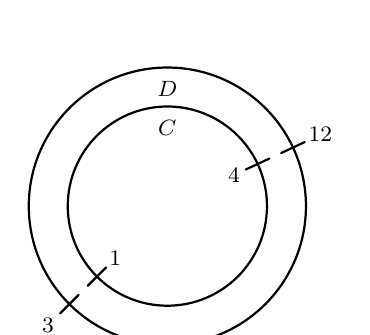
\begin{tikzpicture}[scale=1.1, line cap=round, line join=round]
    \draw[thick] (0, 0) circle (1.6cm);
    \draw[thick] (0, 0) circle (1.15cm);
    
    \node at (0, 1.35) {\footnotesize $D$};
    \node at (0, 0.9) {\footnotesize $C$};
    
    \draw[thick] (25:1.0) -- (25:1.3);
    \draw[thick] (25:1.45) -- (25:1.75);
    \node at (25:0.85) {\footnotesize $4$};
    \node at (25:1.95) {\footnotesize $12$};
    
    \draw[thick] (225:1.0) -- (225:1.3);
    \draw[thick] (225:1.45) -- (225:1.75);
    \node at (225:0.85) {\footnotesize $1$};
    \node at (225:1.95) {\footnotesize $3$};
\end{tikzpicture}
\end{center}

\subsubsection*{習題 5-7}
\begin{enumerate}
    \item 應用 D 尺及 K 尺求下列各數的立方：
    \begin{enumerate}[(i)]
        \item $2.14$,
        \item $5$,
        \item $2.72$,
        \item $3.66$。
    \end{enumerate}
    \item 應用 D 尺及 K 尺求下列各數的立方根：
    \begin{enumerate}[(i)]
        \item $10$,
        \item $100$,
        \item $343$,
        \item $493$。
    \end{enumerate}
    \item 欲求 $x, y$ 的幾何平均，請寫出用計算尺運算的程序。
    \item 自己試着造一根計算尺。
    \item 假設 $L, M, N$ 是三條對數尺度的直線，互相平行，且有相同距離，如下圖所示。在 $L, N$ 兩線上各取點 $x, z$，連接 $xz$ 交 $M$ 線於 $y$ 點，求 $y$ 和 $x, z$ 的關係。
    
    \begin{center}
    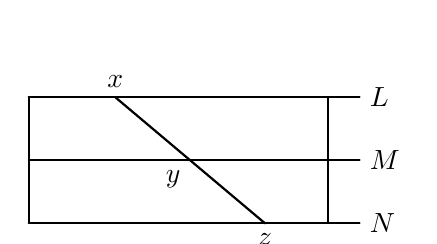
\begin{tikzpicture}[scale=1.0, line cap=round, line join=round]
        \draw[thick] (0, 0) rectangle (3.8, 1.6);
        \draw[thick] (0, 1.6) -- (4.2, 1.6) node[right] {$L$};
        \draw[thick] (0, 0.8) -- (4.2, 0.8) node[right] {$M$};
        \draw[thick] (0, 0) -- (4.2, 0) node[right] {$N$};
        
        \coordinate (X) at (1.1, 1.6);
        \coordinate (Y) at (2.05, 0.8);
        \coordinate (Z) at (3.0, 0);
        \draw[thick] (X) -- (Z);
        
        \node[above] at (X) {$x$};
        \node[below left] at (Y) {$y$};
        \node[below] at (Z) {$z$};
    \end{tikzpicture}
    \end{center}
    
    \item 如圖，兩平行線 $AC$ 及 $BD$ 交一角 $LOM$ 的兩邊於 $A, C, B, D$，若用 $x, y, u, v$, 各表示 $\overline{OA}, \overline{OB}, \overline{OC}, \overline{OD}$，則
    \[
    x : y = u : v, \text{ 卽 } xv = yu.
    \]
    想想看如何利用這個式子造出一個乘除用的計算器械！
    
    \begin{center}
    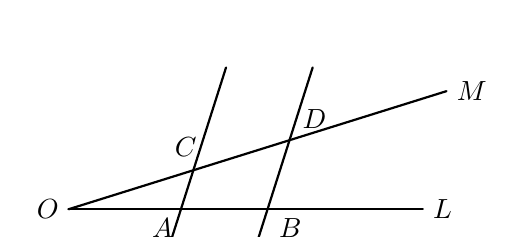
\begin{tikzpicture}[scale=1.0, line cap=round, line join=round]
        \coordinate (O) at (0, 0);
        \draw[thick] (O) -- (4.5, 0) node[right] {$L$};
        \draw[thick] (O) -- (4.8, 1.5) node[right] {$M$};
        \node[left] at (O) {$O$};
        
        \draw[thick] (1.3, -0.4) -- (2.0, 1.8);
        \draw[thick] (2.4, -0.4) -- (3.1, 1.8);
        
        \node[below left] at (1.45, 0) {$A$};
        \node[below right] at (2.55, 0) {$B$};
        \node[above left] at (1.75, 0.55) {$C$};
        \node[above right] at (2.85, 0.9) {$D$};
    \end{tikzpicture}
    \end{center}
\end{enumerate}

\clearpage
\subsection*{附錄：常用對數表}
\addcontentsline{toc}{subsection}{附錄：常用對數表}

\subsubsection*{對數表（1）}
{\centering\fontsize{7.5pt}{8.8pt}\selectfont\setlength{\tabcolsep}{1.5pt}\renewcommand{\arraystretch}{0.96}
\begin{tabular}{|c|cccccccccc|ccccccccc|}
\hline
數 & 0 & 1 & 2 & 3 & 4 & 5 & 6 & 7 & 8 & 9 & 1 & 2 & 3 & 4 & 5 & 6 & 7 & 8 & 9 \\ \hline
1.0 & .0000 & .0043 & .0086 & .0128 & .0170 & .0212 & .0253 & .0294 & .0334 & .0374 & 4 & 8 & 12 & 17 & 21 & 25 & 29 & 33 & 37 \\
1.1 & .0414 & .0453 & .0492 & .0531 & .0569 & .0607 & .0645 & .0682 & .0719 & .0755 & 4 & 8 & 11 & 15 & 19 & 23 & 26 & 30 & 34 \\
1.2 & .0792 & .0828 & .0864 & .0899 & .0934 & .0969 & .1004 & .1038 & .1072 & .1106 & 3 & 7 & 10 & 14 & 17 & 21 & 24 & 28 & 31 \\
1.3 & .1139 & .1173 & .1206 & .1239 & .1271 & .1303 & .1335 & .1367 & .1399 & .1430 & 3 & 6 & 10 & 13 & 16 & 19 & 23 & 26 & 29 \\
1.4 & .1461 & .1492 & .1523 & .1553 & .1584 & .1614 & .1644 & .1673 & .1703 & .1732 & 3 & 6 & 9 & 12 & 15 & 18 & 21 & 24 & 27 \\
1.5 & .1761 & .1790 & .1818 & .1847 & .1875 & .1903 & .1931 & .1959 & .1987 & .2014 & 3 & 6 & 8 & 11 & 14 & 17 & 20 & 22 & 25 \\
1.6 & .2041 & .2068 & .2095 & .2122 & .2148 & .2175 & .2201 & .2227 & .2253 & .2279 & 3 & 5 & 8 & 11 & 13 & 16 & 18 & 21 & 24 \\
1.7 & .2304 & .2330 & .2355 & .2380 & .2405 & .2430 & .2455 & .2480 & .2504 & .2529 & 2 & 5 & 7 & 10 & 12 & 15 & 17 & 20 & 22 \\
1.8 & .2553 & .2577 & .2601 & .2625 & .2648 & .2672 & .2695 & .2718 & .2742 & .2765 & 2 & 5 & 7 & 9 & 12 & 14 & 16 & 19 & 21 \\
1.9 & .2788 & .2810 & .2833 & .2856 & .2878 & .2900 & .2923 & .2945 & .2967 & .2989 & 2 & 4 & 7 & 9 & 11 & 13 & 16 & 18 & 20 \\
2.0 & .3010 & .3032 & .3054 & .3075 & .3096 & .3118 & .3139 & .3160 & .3181 & .3201 & 2 & 4 & 6 & 8 & 11 & 13 & 15 & 17 & 19 \\
2.1 & .3222 & .3243 & .3263 & .3284 & .3304 & .3324 & .3345 & .3365 & .3385 & .3404 & 2 & 4 & 6 & 8 & 10 & 12 & 14 & 16 & 18 \\
2.2 & .3424 & .3444 & .3464 & .3483 & .3502 & .3522 & .3541 & .3560 & .3579 & .3598 & 2 & 4 & 6 & 8 & 10 & 12 & 14 & 15 & 17 \\
2.3 & .3617 & .3636 & .3655 & .3674 & .3692 & .3711 & .3729 & .3747 & .3766 & .3784 & 2 & 4 & 6 & 7 & 9 & 11 & 13 & 15 & 17 \\
2.4 & .3802 & .3820 & .3838 & .3856 & .3874 & .3892 & .3909 & .3927 & .3945 & .3962 & 2 & 4 & 5 & 7 & 9 & 11 & 12 & 14 & 16 \\
2.5 & .3979 & .3997 & .4014 & .4031 & .4048 & .4065 & .4082 & .4099 & .4116 & .4133 & 2 & 3 & 5 & 7 & 9 & 10 & 12 & 14 & 15 \\
2.6 & .4150 & .4166 & .4183 & .4200 & .4216 & .4232 & .4249 & .4265 & .4281 & .4298 & 2 & 3 & 5 & 7 & 8 & 10 & 11 & 13 & 15 \\
2.7 & .4314 & .4330 & .4346 & .4362 & .4378 & .4393 & .4409 & .4425 & .4440 & .4456 & 2 & 3 & 5 & 6 & 8 & 9 & 11 & 13 & 14 \\
2.8 & .4472 & .4487 & .4502 & .4518 & .4533 & .4548 & .4564 & .4579 & .4594 & .4609 & 2 & 3 & 5 & 6 & 8 & 9 & 11 & 12 & 14 \\
2.9 & .4624 & .4639 & .4654 & .4669 & .4683 & .4698 & .4713 & .4728 & .4742 & .4757 & 1 & 3 & 4 & 6 & 7 & 9 & 10 & 12 & 13 \\
3.0 & .4771 & .4786 & .4800 & .4814 & .4829 & .4843 & .4857 & .4871 & .4886 & .4900 & 1 & 3 & 4 & 6 & 7 & 9 & 10 & 11 & 13 \\
3.1 & .4914 & .4928 & .4942 & .4955 & .4969 & .4983 & .4997 & .5011 & .5024 & .5038 & 1 & 3 & 4 & 6 & 7 & 8 & 10 & 11 & 12 \\
3.2 & .5051 & .5065 & .5079 & .5092 & .5105 & .5119 & .5132 & .5145 & .5159 & .5172 & 1 & 3 & 4 & 5 & 7 & 8 & 9 & 11 & 12 \\
3.3 & .5185 & .5198 & .5211 & .5224 & .5237 & .5250 & .5263 & .5276 & .5289 & .5302 & 1 & 3 & 4 & 5 & 6 & 8 & 9 & 10 & 12 \\
3.4 & .5315 & .5328 & .5340 & .5353 & .5366 & .5378 & .5391 & .5403 & .5416 & .5428 & 1 & 3 & 4 & 5 & 6 & 8 & 9 & 10 & 11 \\
3.5 & .5441 & .5453 & .5465 & .5478 & .5490 & .5502 & .5514 & .5527 & .5539 & .5551 & 1 & 2 & 4 & 5 & 6 & 7 & 9 & 10 & 11 \\
3.6 & .5563 & .5575 & .5587 & .5599 & .5611 & .5623 & .5635 & .5647 & .5658 & .5670 & 1 & 2 & 4 & 5 & 6 & 7 & 8 & 10 & 11 \\
3.7 & .5682 & .5694 & .5705 & .5717 & .5729 & .5740 & .5752 & .5763 & .5775 & .5786 & 1 & 2 & 3 & 5 & 6 & 7 & 8 & 9 & 10 \\
3.8 & .5798 & .5809 & .5821 & .5832 & .5843 & .5855 & .5866 & .5877 & .5888 & .5899 & 1 & 2 & 3 & 5 & 6 & 7 & 8 & 9 & 10 \\
3.9 & .5911 & .5922 & .5933 & .5944 & .5955 & .5966 & .5977 & .5988 & .5999 & .6010 & 1 & 2 & 3 & 4 & 5 & 7 & 8 & 9 & 10 \\
4.0 & .6021 & .6031 & .6042 & .6053 & .6064 & .6075 & .6085 & .6096 & .6107 & .6117 & 1 & 2 & 3 & 4 & 5 & 6 & 8 & 9 & 10 \\
4.1 & .6128 & .6138 & .6149 & .6160 & .6170 & .6180 & .6191 & .6201 & .6212 & .6222 & 1 & 2 & 3 & 4 & 5 & 6 & 7 & 8 & 9 \\
4.2 & .6232 & .6243 & .6253 & .6263 & .6274 & .6284 & .6294 & .6304 & .6314 & .6325 & 1 & 2 & 3 & 4 & 5 & 6 & 7 & 8 & 9 \\
4.3 & .6335 & .6345 & .6355 & .6365 & .6375 & .6385 & .6395 & .6405 & .6415 & .6425 & 1 & 2 & 3 & 4 & 5 & 6 & 7 & 8 & 9 \\
4.4 & .6435 & .6444 & .6454 & .6464 & .6474 & .6484 & .6493 & .6503 & .6513 & .6522 & 1 & 2 & 3 & 4 & 5 & 6 & 7 & 8 & 9 \\
4.5 & .6532 & .6542 & .6551 & .6561 & .6571 & .6580 & .6590 & .6599 & .6609 & .6618 & 1 & 2 & 3 & 4 & 5 & 6 & 7 & 8 & 9 \\
4.6 & .6628 & .6637 & .6646 & .6656 & .6665 & .6675 & .6684 & .6693 & .6702 & .6712 & 1 & 2 & 3 & 4 & 5 & 6 & 7 & 7 & 8 \\
4.7 & .6721 & .6730 & .6739 & .6749 & .6758 & .6767 & .6776 & .6785 & .6794 & .6803 & 1 & 2 & 3 & 4 & 5 & 5 & 6 & 7 & 8 \\
4.8 & .6812 & .6821 & .6830 & .6839 & .6848 & .6857 & .6866 & .6875 & .6884 & .6893 & 1 & 2 & 3 & 4 & 4 & 5 & 6 & 7 & 8 \\
4.9 & .6902 & .6911 & .6920 & .6928 & .6937 & .6946 & .6955 & .6964 & .6972 & .6981 & 1 & 2 & 3 & 4 & 4 & 5 & 6 & 7 & 8 \\
5.0 & .6990 & .6998 & .7007 & .7016 & .7024 & .7033 & .7042 & .7050 & .7059 & .7067 & 1 & 2 & 3 & 3 & 4 & 5 & 6 & 7 & 8 \\
5.1 & .7076 & .7084 & .7093 & .7101 & .7110 & .7118 & .7126 & .7135 & .7143 & .7152 & 1 & 2 & 3 & 3 & 4 & 5 & 6 & 7 & 8 \\
5.2 & .7160 & .7168 & .7177 & .7185 & .7193 & .7202 & .7210 & .7218 & .7226 & .7235 & 1 & 2 & 2 & 3 & 4 & 5 & 6 & 7 & 7 \\
5.3 & .7243 & .7251 & .7259 & .7267 & .7275 & .7284 & .7292 & .7300 & .7308 & .7316 & 1 & 2 & 2 & 3 & 4 & 5 & 6 & 6 & 7 \\
5.4 & .7324 & .7332 & .7340 & .7348 & .7356 & .7364 & .7372 & .7380 & .7388 & .7396 & 1 & 2 & 2 & 3 & 4 & 5 & 6 & 6 & 7 \\
\hline
\end{tabular}\par}

\vspace{0.5em}
\noindent $\log \pi = 0.4971$

\clearpage
\subsubsection*{對數表（2）}
{\centering\fontsize{7.5pt}{8.8pt}\selectfont\setlength{\tabcolsep}{1.5pt}\renewcommand{\arraystretch}{0.96}
\begin{tabular}{|c|cccccccccc|ccccccccc|}
\hline
數 & 0 & 1 & 2 & 3 & 4 & 5 & 6 & 7 & 8 & 9 & 1 & 2 & 3 & 4 & 5 & 6 & 7 & 8 & 9 \\ \hline
5.5 & .7404 & .7412 & .7419 & .7427 & .7435 & .7443 & .7451 & .7459 & .7466 & .7474 & 1 & 2 & 2 & 3 & 4 & 5 & 5 & 6 & 7 \\
5.6 & .7482 & .7490 & .7497 & .7505 & .7513 & .7520 & .7528 & .7536 & .7543 & .7551 & 1 & 2 & 2 & 3 & 4 & 5 & 5 & 6 & 7 \\
5.7 & .7559 & .7566 & .7574 & .7582 & .7589 & .7597 & .7604 & .7612 & .7619 & .7627 & 1 & 2 & 2 & 3 & 4 & 5 & 5 & 6 & 7 \\
5.8 & .7634 & .7642 & .7649 & .7657 & .7664 & .7672 & .7679 & .7686 & .7694 & .7701 & 1 & 1 & 2 & 3 & 4 & 4 & 5 & 6 & 7 \\
5.9 & .7709 & .7716 & .7723 & .7731 & .7738 & .7745 & .7752 & .7760 & .7767 & .7774 & 1 & 1 & 2 & 3 & 4 & 4 & 5 & 6 & 7 \\
6.0 & .7782 & .7789 & .7796 & .7803 & .7810 & .7818 & .7825 & .7832 & .7839 & .7846 & 1 & 1 & 2 & 3 & 4 & 4 & 5 & 6 & 6 \\
6.1 & .7853 & .7860 & .7868 & .7875 & .7882 & .7889 & .7896 & .7903 & .7910 & .7917 & 1 & 1 & 2 & 3 & 4 & 4 & 5 & 6 & 6 \\
6.2 & .7924 & .7931 & .7938 & .7945 & .7952 & .7959 & .7966 & .7973 & .7980 & .7987 & 1 & 1 & 2 & 3 & 3 & 4 & 5 & 6 & 6 \\
6.3 & .7993 & .8000 & .8007 & .8014 & .8021 & .8028 & .8035 & .8041 & .8048 & .8055 & 1 & 1 & 2 & 3 & 3 & 4 & 5 & 5 & 6 \\
6.4 & .8062 & .8069 & .8075 & .8082 & .8089 & .8096 & .8102 & .8109 & .8116 & .8122 & 1 & 1 & 2 & 3 & 3 & 4 & 5 & 5 & 6 \\
6.5 & .8129 & .8136 & .8142 & .8149 & .8156 & .8162 & .8169 & .8176 & .8182 & .8189 & 1 & 1 & 2 & 3 & 3 & 4 & 5 & 5 & 6 \\
6.6 & .8195 & .8202 & .8209 & .8215 & .8222 & .8228 & .8235 & .8241 & .8248 & .8254 & 1 & 1 & 2 & 3 & 3 & 4 & 5 & 5 & 6 \\
6.7 & .8261 & .8267 & .8274 & .8280 & .8287 & .8293 & .8299 & .8306 & .8312 & .8319 & 1 & 1 & 2 & 3 & 3 & 4 & 5 & 5 & 6 \\
6.8 & .8325 & .8331 & .8338 & .8344 & .8351 & .8357 & .8363 & .8370 & .8376 & .8382 & 1 & 1 & 2 & 3 & 3 & 4 & 4 & 5 & 6 \\
6.9 & .8388 & .8395 & .8401 & .8407 & .8414 & .8420 & .8426 & .8432 & .8439 & .8445 & 1 & 1 & 2 & 2 & 3 & 4 & 4 & 5 & 6 \\
7.0 & .8451 & .8457 & .8463 & .8470 & .8476 & .8482 & .8488 & .8494 & .8500 & .8506 & 1 & 1 & 2 & 2 & 3 & 4 & 4 & 5 & 6 \\
7.1 & .8513 & .8519 & .8525 & .8531 & .8537 & .8543 & .8549 & .8555 & .8561 & .8567 & 1 & 1 & 2 & 2 & 3 & 4 & 4 & 5 & 5 \\
7.2 & .8573 & .8579 & .8585 & .8591 & .8597 & .8603 & .8609 & .8615 & .8621 & .8627 & 1 & 1 & 2 & 2 & 3 & 4 & 4 & 5 & 5 \\
7.3 & .8633 & .8639 & .8645 & .8651 & .8657 & .8663 & .8669 & .8675 & .8681 & .8686 & 1 & 1 & 2 & 2 & 3 & 4 & 4 & 5 & 5 \\
7.4 & .8692 & .8698 & .8704 & .8710 & .8716 & .8722 & .8727 & .8733 & .8739 & .8745 & 1 & 1 & 2 & 2 & 3 & 3 & 4 & 5 & 5 \\
7.5 & .8751 & .8756 & .8762 & .8768 & .8774 & .8779 & .8785 & .8791 & .8797 & .8802 & 1 & 1 & 2 & 2 & 3 & 3 & 4 & 5 & 5 \\
7.6 & .8808 & .8814 & .8820 & .8825 & .8831 & .8837 & .8842 & .8848 & .8854 & .8859 & 1 & 1 & 2 & 2 & 3 & 3 & 4 & 5 & 5 \\
7.7 & .8865 & .8871 & .8876 & .8882 & .8887 & .8893 & .8899 & .8904 & .8910 & .8915 & 1 & 1 & 2 & 2 & 3 & 3 & 4 & 4 & 5 \\
7.8 & .8921 & .8927 & .8932 & .8938 & .8943 & .8949 & .8954 & .8960 & .8965 & .8971 & 1 & 1 & 2 & 2 & 3 & 3 & 4 & 4 & 5 \\
7.9 & .8976 & .8982 & .8987 & .8993 & .8998 & .9004 & .9009 & .9015 & .9020 & .9025 & 1 & 1 & 2 & 2 & 3 & 3 & 4 & 4 & 5 \\
8.0 & .9031 & .9036 & .9042 & .9047 & .9053 & .9058 & .9063 & .9069 & .9074 & .9079 & 1 & 1 & 2 & 2 & 3 & 3 & 4 & 4 & 5 \\
8.1 & .9085 & .9090 & .9096 & .9101 & .9106 & .9112 & .9117 & .9122 & .9128 & .9133 & 1 & 1 & 2 & 2 & 3 & 3 & 4 & 4 & 5 \\
8.2 & .9138 & .9143 & .9149 & .9154 & .9159 & .9165 & .9170 & .9175 & .9180 & .9186 & 1 & 1 & 2 & 2 & 3 & 3 & 4 & 4 & 5 \\
8.3 & .9191 & .9196 & .9201 & .9206 & .9212 & .9217 & .9222 & .9227 & .9232 & .9238 & 1 & 1 & 2 & 2 & 3 & 3 & 4 & 4 & 5 \\
8.4 & .9243 & .9248 & .9253 & .9258 & .9263 & .9269 & .9274 & .9279 & .9284 & .9289 & 1 & 1 & 2 & 2 & 3 & 3 & 4 & 4 & 5 \\
8.5 & .9294 & .9299 & .9304 & .9309 & .9315 & .9320 & .9325 & .9330 & .9335 & .9340 & 1 & 1 & 2 & 2 & 3 & 3 & 4 & 4 & 5 \\
8.6 & .9345 & .9350 & .9355 & .9360 & .9365 & .9370 & .9375 & .9380 & .9385 & .9390 & 1 & 1 & 2 & 2 & 3 & 3 & 4 & 4 & 5 \\
8.7 & .9395 & .9400 & .9405 & .9410 & .9415 & .9420 & .9425 & .9430 & .9435 & .9440 & 0 & 1 & 1 & 2 & 2 & 3 & 3 & 4 & 4 \\
8.8 & .9445 & .9450 & .9455 & .9460 & .9465 & .9469 & .9474 & .9479 & .9484 & .9489 & 0 & 1 & 1 & 2 & 2 & 3 & 3 & 4 & 4 \\
8.9 & .9494 & .9499 & .9504 & .9509 & .9513 & .9518 & .9523 & .9528 & .9533 & .9538 & 0 & 1 & 1 & 2 & 2 & 3 & 3 & 4 & 4 \\
9.0 & .9542 & .9547 & .9552 & .9557 & .9562 & .9566 & .9571 & .9576 & .9581 & .9586 & 0 & 1 & 1 & 2 & 2 & 3 & 3 & 4 & 4 \\
9.1 & .9590 & .9595 & .9600 & .9605 & .9609 & .9614 & .9619 & .9624 & .9628 & .9633 & 0 & 1 & 1 & 2 & 2 & 3 & 3 & 4 & 4 \\
9.2 & .9638 & .9643 & .9647 & .9652 & .9657 & .9661 & .9666 & .9671 & .9675 & .9680 & 0 & 1 & 1 & 2 & 2 & 3 & 3 & 4 & 4 \\
9.3 & .9685 & .9689 & .9694 & .9699 & .9703 & .9708 & .9713 & .9717 & .9722 & .9727 & 0 & 1 & 1 & 2 & 2 & 3 & 3 & 4 & 4 \\
9.4 & .9731 & .9736 & .9741 & .9745 & .9750 & .9754 & .9759 & .9763 & .9768 & .9773 & 0 & 1 & 1 & 2 & 2 & 3 & 3 & 4 & 4 \\
9.5 & .9777 & .9782 & .9786 & .9791 & .9795 & .9800 & .9805 & .9809 & .9814 & .9818 & 0 & 1 & 1 & 2 & 2 & 3 & 3 & 4 & 4 \\
9.6 & .9823 & .9827 & .9832 & .9836 & .9841 & .9845 & .9850 & .9854 & .9859 & .9863 & 0 & 1 & 1 & 2 & 2 & 3 & 3 & 4 & 4 \\
9.7 & .9868 & .9872 & .9877 & .9881 & .9886 & .9890 & .9894 & .9899 & .9903 & .9908 & 0 & 1 & 1 & 2 & 2 & 3 & 3 & 4 & 4 \\
9.8 & .9912 & .9917 & .9921 & .9926 & .9930 & .9934 & .9939 & .9943 & .9948 & .9952 & 0 & 1 & 1 & 2 & 2 & 3 & 3 & 4 & 4 \\
9.9 & .9956 & .9961 & .9965 & .9969 & .9974 & .9978 & .9983 & .9987 & .9991 & .9996 & 0 & 1 & 1 & 2 & 2 & 3 & 3 & 3 & 4 \\
\hline
\end{tabular}\par}
 % 第五章 對數表的用法與計算尺原理*

\end{document}
